\documentclass[12pt]{article}

\usepackage[dvipsnames]{xcolor}
\usepackage[figuresright]{rotating}
\usepackage[margin=1in]{geometry}
\usepackage[pdftex]{lscape}
\usepackage[spanish]{babel}
\usepackage[utf8]{inputenc}
\usepackage{amsmath, amssymb}
\usepackage{amsmath,amssymb,amsthm,amsfonts}
\usepackage{amsmath}
\usepackage{amssymb}
\usepackage{anysize}
\usepackage{color}
\usepackage{enumerate}
\usepackage{fancyhdr}
\usepackage{float}
\usepackage{geometry}
\usepackage{graphicx,graphics}
\usepackage{graphicx}
\usepackage{hyperref}
\usepackage{imakeidx}
\usepackage{listings}
\usepackage{longtable}
\usepackage{multicol}
\usepackage{multirow}
\usepackage{rotating}
\usepackage{subfig}
\usepackage{tikz}
\usepackage{titlesec}
\usepackage{url}
\usetikzlibrary{shapes, arrows, positioning}

%\geometry{margin=1in}
%\usepackage[margin=0.75in]{geometry}  % Ajustar márgenes


\newtheorem{Def}{Definici\'on}[section]
\newtheorem{Ejem}{Ejemplo}[section]
\newtheorem{Teo}{Teorema}[section]
\newtheorem{Dem}{Demostraci\'on}[section]
\newtheorem{Note}{Nota}%[section]
\newtheorem{Sol}{Soluci\'on}[section]
\newtheorem{Prop}{Proposici\'on}[section]
\newtheorem{Coro}{Corolario}[section]
\newtheorem{Quest}{Pregunta}[section]
\newtheorem{Criterio}{Criterio}%[section]
\newtheorem{Sup}{Supuesto}%[section]



\title{Random Forest and Deep Learning}
\author{Carlos E Mart\'inez-Rodr\'iguez}
\date{14  de noviembre de 2023}  % Eliminar la fecha automática

\begin{document}

\maketitle
\tableofcontents

\newpage
%== == ==  == == == ==  == == == ==  == == == ==  == == == ==  == 
\section{Bioinformatics: New revision}
%== == ==  == == == ==  == == == ==  == == == ==  == == == ==  == 

%-- -- -- -- -- -- -- -- -- -- -- -- -- -- -- -- -- -- -- -- -- -- -- -- -- -- -- -- -- -- 
\subsection{A bayesian framework for combining gene predictions - Pavlovic}
%-- -- -- -- -- -- -- -- -- -- -- -- -- -- -- -- -- -- -- -- -- -- -- -- -- -- -- -- -- -- 

Biology and biotechnology are undergoing a techonolgical revolution which is transforming research into an information-rich enterprise.  A typical bacterial genome sequence is comprised of several million bases of DNA and contains several thousand genes. The human genome is approximately 3 billion bases long and it contains approximately 30,000 putative genes identified thus far.



%== == ==  == == == ==  == == == ==  == == == ==  == == == ==  == 
\section{Random Forest: Explanation in Mathematical Terms}

Random Forest is a supervised learning algorithm used for both classification and regression problems. The main idea behind Random Forest is to build multiple decision trees during training and combine their results to obtain a more robust and accurate prediction.

Let's assume we have a training dataset \(D = \{(x_1, y_1), (x_2, y_2), \ldots, (x_n, y_n)\}\), where \(x_i\) represents the features and \(y_i\) is the target variable.

\begin{enumerate}
    \item \textbf{Construction of Decision Trees:}
        \begin{itemize}
            \item For each tree, a random subset of features is selected (randomly sample features), and a random subset of training data is chosen (randomly sample observations with replacement).
            \item A decision tree is constructed using the subset of data and features.
            \item The decision tree is represented as \(h_i(x;\theta_i)\), where \(i\) denotes the tree index, \(x\) is the input feature vector, and \(\theta_i\) represents the parameters of the tree.
            \item At each node \(t\) of the tree, a feature \(j_t\) is selected from the random subset, and the split is determined based on minimizing impurity:
            \[
            \theta_{i,t} = \arg\min_{j_t, s_t} \left[\textrm{Impurity}(D_t) - p_{\textrm{left}}\textrm{Impurity}(D_{\textrm{left}}) - p_{\textrm{right}}\textrm{Impurity}(D_{\textrm{right}})\right]
            \]
            where \(D_t\) is the dataset at node \(t\), \(D_{\textrm{left}}\) and \(D_{\textrm{right}}\) are the datasets in the left and right child nodes, \(p_{\textrm{left}}\) and \(p_{\textrm{right}}\) are the proportions of data in the left and right child nodes, and \(\textrm{Impurity}(\cdot)\) is a measure of impurity, such as Gini index for classification or mean squared error for regression.
        \end{itemize}
    
    \item \textbf{Voting or Averaging:}
        \begin{itemize}
            \item For classification problems, the final prediction is obtained by majority voting among the trees:
            \[
            H(x) = \textrm{mode}\{h_1(x;\theta_1), h_2(x;\theta_2), \ldots, h_n(x;\theta_n)\}
            \]
            \item For regression problems, the final prediction is the average of predictions from all trees:
            \[
            H(x) = \frac{1}{n}\sum_{i=1}^{n}h_i(x;\theta_i)
            \]
        \end{itemize}
    
    \item \textbf{Variance Reduction:}
        \begin{itemize}
            \item By building decision trees in a random manner, the variance of the model is reduced, leading to a more robust and generalizable model.
        \end{itemize}
\end{enumerate}

The final prediction is obtained by combining the predictions of all trees.

\section{Deep Learning: Overview}

Deep Learning is a subfield of machine learning that focuses on neural networks with multiple layers (deep neural networks). These networks can automatically learn hierarchical representations of data, allowing them to capture intricate patterns and features.

\begin{enumerate}
    \item \textbf{Neural Network Representation:}
        \begin{itemize}
            \item A neural network consists of layers of interconnected nodes (neurons) organized into an input layer, one or more hidden layers, and an output layer.
            \item The input layer represents the features of the data, and each neuron in the layer processes a specific feature.
            \item Hidden layers perform nonlinear transformations on the input data, learning hierarchical representations.
            \item The output layer produces the final prediction based on the learned representations.
        \end{itemize}
    
    \item \textbf{Training a Neural Network:}
        \begin{itemize}
            \item During training, the network's parameters (weights and biases) are adjusted to minimize the difference between predicted and actual outputs.
            \item This optimization is typically done using backpropagation and gradient descent.
        \end{itemize}
    
    \item \textbf{Activation Functions:}
        \begin{itemize}
            \item Activation functions introduce nonlinearity to the neural network, enabling it to learn complex patterns.
            \item Common activation functions include ReLU (Rectified Linear Unit), Sigmoid, and Hyperbolic Tangent (tanh).
        \end{itemize}
    
    \item \textbf{Forward Pass:}
        \begin{itemize}
            \item The forward pass of a neural network involves computing the output of the network for a given input.
            \item Given an input vector \(x\), the output \(y\) is computed by passing \(x\) through the network's layers using learned weights and biases.
            \item The output of each layer is computed as:
            \[
            a^{(l)} = W^{(l)}a^{(l-1)} + b^{(l)}
            \]
            where \(W^{(l)}\) is the weight matrix, \(a^{(l)}\) is the activation of layer \(l\), \(a^{(l-1)}\) is the activation of the previous layer, and \(b^{(l)}\) is the bias vector.
            \item The activation function is then applied to \(a^{(l)}\) to introduce nonlinearity.
        \end{itemize}
    
    \item \textbf{Loss Function:}
        \begin{itemize}
            \item The loss function measures the difference between the predicted output and the true output.
            \item Common loss functions include mean squared error for regression and cross-entropy for classification.
            \item The goal during training is to minimize the loss by adjusting the network's parameters.
        \end{itemize}
    
    \item \textbf{Backpropagation:}
        \begin{itemize}
            \item Backpropagation is a training algorithm that computes the gradient of the loss with respect to the network's parameters.
            \item The gradient is used to update the parameters in the direction that reduces the loss.
            \item It involves computing the gradient of the loss with respect to the output of each layer and using the chain rule to propagate these gradients backward through the network.
        \end{itemize}
\end{enumerate}

\section{Example of Implementation in R:}

\subsection{Install and Load the Keras Library:}
\begin{verbatim}
install.packages("keras")
library(keras)
\end{verbatim}

\subsection{Build a Simple Neural Network:}
\begin{verbatim}
model <- keras_model_sequential() %>%
  layer_dense(units = 128, activation = 'relu', input_shape = c(10)) %>%
  layer_dense(units = 1, activation = 'sigmoid')

summary(model)
\end{verbatim}

\subsection{Compile and Train the Neural Network:}
\begin{verbatim}
model %>% compile(
  optimizer = 'adam',
  loss = 'binary_crossentropy',
  metrics = c('accuracy')
)

# Assuming you have training data X_train and labels y_train
history <- model %>% fit(
  X_train, y_train,
  epochs = 10, batch_size = 32,
  validation_split = 0.2
)
\end{verbatim}

\subsection{Evaluate the Model:}
\begin{verbatim}
# Assuming you have test data X_test and labels y_test
evaluate_result <- model %>% evaluate(X_test, y_test)
print(evaluate_result)
\end{verbatim}


\section{Impurity Measures in Random Forest}

In the context of Random Forest, impurity measures play a crucial role in the construction of decision trees. The two commonly used impurity measures are the Gini index for classification and the mean squared error for regression.

\subsection{Gini Index for Classification}

The Gini index is a measure of impurity used in classification problems. Given a node in a decision tree that contains data points from different classes, the Gini index quantifies how often a randomly chosen data point would be incorrectly classified.

For a node \(t\) with \(K\) classes and a set of data points \(D_t\), the Gini index (\(Gini(t)\)) is calculated as follows:

\[ Gini(t) = 1 - \sum_{i=1}^{K} p_i^2 \]

where \(p_i\) is the proportion of data points in class \(i\) at node \(t\). A lower Gini index indicates a purer node with predominantly one class.

In the context of Random Forest, the decision tree split is determined by minimizing the weighted sum of Gini indices for the left and right child nodes. The split that results in the lowest overall Gini index is chosen.

\subsection{Mean Squared Error for Regression}

For regression problems, the impurity measure used is the mean squared error (MSE). Unlike classification, where impurity is related to the purity of classes in a node, regression impurity is a measure of the variability of target values within a node.

For a node \(t\) with data points \(D_t\), the MSE (\(MSE(t)\)) is calculated as follows:

\[ MSE(t) = \frac{1}{|D_t|} \sum_{i \in D_t} (y_i - \bar{y}_t)^2 \]

where \(y_i\) is the target value of data point \(i\), \(|D_t|\) is the number of data points in node \(t\), and \(\bar{y}_t\) is the mean target value of all data points in node \(t\).

Similar to the Gini index, in Random Forest, the decision tree split is determined by minimizing the weighted sum of MSE for the left and right child nodes.

These impurity measures guide the construction of individual decision trees within the Random Forest ensemble, contributing to the overall robustness and predictive power of the model.


\section{Construcción del Árbol de Decisión}

\subsection{Teoría:}

Un árbol de decisión es una estructura de datos que representa un conjunto de decisiones y sus posibles consecuencias. En el contexto de Random Forest, la construcción de un árbol de decisión sigue el principio de "aprendizaje supervisado", donde el algoritmo aprende patrones a partir de un conjunto de datos etiquetado.

La construcción del árbol se realiza a través de divisiones recursivas basadas en características del conjunto de datos. Cada nodo del árbol representa una pregunta sobre una característica, y las ramas que surgen de ese nodo son las respuestas a esa pregunta. El proceso continúa hasta que se alcanza un criterio de parada, como la profundidad máxima del árbol o el número mínimo de muestras en un nodo.

\subsection{Elementos Matemáticos:}

1. \textbf{Función de Impureza:}

En cada nodo del árbol, se elige la característica y el umbral que minimizan la impureza en los nodos hijos resultantes. La impureza se mide mediante funciones como el Índice de Gini para clasificación o el Error Cuadrático Medio (MSE) para regresión.

Para clasificación:
\[ Gini(t) = 1 - \sum_{i=1}^{K} p_i^2 \]

Donde \( p_i \) es la proporción de ejemplos de la clase \( i \) en el nodo \( t \).

Para regresión:
\[ MSE(t) = \frac{1}{|D_t|} \sum_{i \in D_t} (y_i - \bar{y}_t)^2 \]

Donde \( D_t \) es el conjunto de datos en el nodo \( t \), \( y_i \) es la etiqueta del ejemplo \( i \), y \( \bar{y}_t \) es la media de las etiquetas en el nodo \( t \).

2. \textbf{Criterio de División:}

La elección de la mejor característica y umbral se basa en la reducción de la impureza. Se busca el par \((j, s)\) que minimiza la expresión:
\[ \theta_{i,t} = \arg\min_{j, s} \left[ \textrm{Impureza}(D_t) - p_{\textrm{left}}\textrm{Impureza}(D_{\textrm{left}}) - p_{\textrm{right}}\textrm{Impureza}(D_{\textrm{right}}) \right] \]

Donde \(D_t\) es el conjunto de datos en el nodo \(t\), \(D_{\textrm{left}}\) y \(D_{\textrm{right}}\) son los conjuntos de datos en los nodos izquierdo y derecho después de la división, y \(p_{\textrm{left}}\) y \(p_{\textrm{right}}\) son las proporciones de datos en esos nodos.

3. \textbf{Criterios de Parada:}

Para evitar sobreajuste, se utilizan criterios de parada, como la profundidad máxima del árbol o el número mínimo de muestras requeridas para realizar una división.

La construcción de cada árbol en Random Forest implica este proceso iterativo y se repite para cada árbol en el bosque. La diversidad en la construcción de árboles se logra mediante el uso de diferentes subconjuntos aleatorios de características y datos en cada árbol. La combinación de predicciones de estos árboles mejora la generalización del modelo y su capacidad predictiva en nuevos datos.



\section{Reducción de Varianza en Random Forest}

\subsection{Teoría:}

La reducción de la varianza es uno de los objetivos clave en la construcción de árboles de decisión en Random Forest. Esta técnica busca mejorar la generalización del modelo al reducir la sensibilidad a pequeñas variaciones en los datos de entrenamiento.

La varianza se refiere a la variabilidad de las predicciones de un modelo respecto a diferentes conjuntos de datos de entrenamiento. En Random Forest, la reducción de la varianza se logra mediante dos técnicas principales: Bagging y Random Subspace.

\subsubsection{Bagging (Bootstrap Aggregating):}

Bagging es una técnica que consiste en entrenar múltiples modelos en diferentes subconjuntos de datos generados mediante muestreo con reemplazo (bootstrap). Cada árbol de decisión en Random Forest se entrena en un conjunto de datos ligeramente diferente, lo que introduce diversidad en los modelos.

\subsubsection{Random Subspace:}

Random Subspace es otra técnica utilizada para reducir la correlación entre los árboles de decisión. En lugar de usar todas las características para cada árbol, se selecciona un subconjunto aleatorio de características para entrenar cada árbol. Esto ayuda a que cada árbol se especialice en diferentes aspectos de los datos, mejorando la diversidad y reduciendo la correlación entre las predicciones.

\subsection{Elementos Matemáticos:}

La reducción de la varianza no se expresa directamente con fórmulas matemáticas específicas, pero los conceptos clave son fundamentales:

1. **Bagging:**
    - Cada árbol \(T_i\) se entrena en un conjunto de datos \(D_i\) generado por muestreo con reemplazo (bootstrap).
    - La predicción final se obtiene promediando las predicciones de todos los árboles:
        \[ H(x) = \frac{1}{N} \sum_{i=1}^{N} T_i(x) \]

2. **Random Subspace:**
    - Cada árbol \(T_i\) se entrena utilizando un subconjunto aleatorio de características.
    - La predicción final se obtiene promediando las predicciones de todos los árboles:
        \[ H(x) = \frac{1}{N} \sum_{i=1}^{N} T_i(x) \]

Estos enfoques combinados contribuyen a reducir la varianza del modelo, lo que resulta en un modelo más robusto y generalizable.

\section{Votación y Promedio en Random Forest}

\subsection{Teoría:}

La técnica de "Votación" (para problemas de clasificación) o "Promedio" (para problemas de regresión) es crucial en Random Forest para combinar las predicciones de múltiples árboles de decisión y obtener una predicción final más robusta y precisa.

\subsubsection{Para Problemas de Clasificación:}

En problemas de clasificación, el enfoque de votación se utiliza. Cada árbol en el bosque emite una predicción de clase, y la clase final se determina por mayoría de votos.

\subsubsection{Para Problemas de Regresión:}

En problemas de regresión, se utiliza un enfoque de promedio. Cada árbol realiza una predicción numérica, y la predicción final es el promedio de todas las predicciones.

\subsection{Elementos Matemáticos:}

1. \textbf{Votación para Clasificación:}
    - La predicción final para un ejemplo \(x\) se obtiene por mayoría de votos:
        \[ H(x) = \textrm{mode}\{T_1(x), T_2(x), ..., T_N(x)\} \]

2. \textbf{Promedio para Regresión:}
    - La predicción final para un ejemplo \(x\) se obtiene promediando las predicciones de todos los árboles:
        \[ H(x) = \frac{1}{N}\sum_{i=1}^{N} T_i(x) \]

Donde \(T_i(x)\) representa la predicción del árbol \(i\) para el ejemplo \(x\), y \(N\) es el número total de árboles en el bosque.

Estos enfoques de votación y promedio permiten que Random Forest combine la información de múltiples árboles de decisión, mejorando la generalización y la capacidad predictiva del modelo.

\section{Resumen}

Random Forest es un algoritmo de aprendizaje automático que se utiliza para resolver problemas de clasificación y regresión. En lugar de utilizar un único árbol de decisión, Random Forest construye varios árboles de decisión y los combina para obtener una predicción más precisa. Cada árbol de decisión se construye utilizando un subconjunto aleatorio de las características del conjunto de datos original. Al final, las predicciones de cada árbol se promedian para obtener una predicción final.

El algoritmo de Random Forest se basa en dos técnicas: Bagging y Random Subspace. Bagging es una técnica que se utiliza para reducir la varianza de un modelo al entrenar múltiples modelos en diferentes subconjuntos de datos. Random Subspace es una técnica que se utiliza para reducir la correlación entre los modelos al entrenar cada modelo en diferentes subconjuntos de características.

Aquí hay algunos elementos matemáticos que se utilizan en Random Forest:

\begin{itemize}
    \item \textbf{Árbol de decisión:} Un árbol de decisión es una estructura de datos que se utiliza para modelar decisiones y sus posibles consecuencias. Cada nodo en el árbol representa una decisión, y cada rama representa una posible consecuencia de esa decisión. Los árboles de decisión se construyen utilizando un conjunto de reglas que se utilizan para tomar decisiones.
    \item \textbf{Bootstrap:} Bootstrap es una técnica que se utiliza para generar múltiples conjuntos de datos a partir de un conjunto de datos original. Cada conjunto de datos se genera mediante muestreo con reemplazo, lo que significa que cada elemento del conjunto de datos original tiene la misma probabilidad de ser seleccionado en cada conjunto de datos generado.
    \item \textbf{Out-of-Bag Error:} Out-of-Bag Error es una técnica que se utiliza para estimar el error de validación de un modelo sin la necesidad de un conjunto de datos de validación separado. El error se estima utilizando los datos que no se incluyeron en el conjunto de datos de entrenamiento para cada árbol de decisión.
\end{itemize}

\subsection{Ejemplo en R: Random Forest}

Aquí hay un ejemplo de cómo construir un modelo de bosque aleatorio en R:

\begin{verbatim}
# Cargamos el paquete necesario para este ejemplo
library(randomForest)

# Cargamos el conjunto de datos que deseamos utilizar
data(iris)

# Dividimos el conjunto de datos en conjuntos de entrenamiento y prueba
trainIndex <- createDataPartition(iris$Species, p = .8, list = FALSE, times = 1)

# Entrenamos el modelo de bosque aleatorio
rf_model <- randomForest(Species ~ ., data = iris[trainIndex,])

# Realizamos predicciones en el conjunto de prueba
predictions <- predict(rf_model, iris[-trainIndex,])
\end{verbatim}

\subsection{Deep Learning}

Deep Learning es un subcampo del aprendizaje automático que se centra en la creación de redes neuronales artificiales profundas. Estas redes neuronales están diseñadas para imitar el cerebro humano y son capaces de aprender patrones complejos en los datos.

Aquí hay un ejemplo de cómo construir una red neuronal profunda en R utilizando el paquete keras:

\begin{verbatim}
# Cargamos los paquetes necesarios
library(keras)
library(tensorflow)

# Cargamos el conjunto de datos que deseamos utilizar
data(iris)

# Dividimos el conjunto de datos en conjuntos de entrenamiento y prueba
trainIndex <- createDataPartition(iris$Species, p = .8, list = FALSE, times = 1)

# Creamos la red neuronal
model <- keras_model_sequential() %>% 
  layer_dense(units = 4, input_shape = c(4)) %>% 
  layer_activation("relu") %>% 
  layer_dense(units = 3) %>% 
  layer_activation("softmax")

# Compilamos la red neuronal
model %>% compile(loss = "categorical_crossentropy", optimizer = "adam", metrics = "accuracy")

# Entrenamos la red neuronal
history <- model %>% fit(
  x = iris[trainIndex, 1:4],
  y = to_categorical(as.numeric(iris[trainIndex, 5])),
  epochs = 100,
  batch_size = 10,
  validation_split = 0.2
)
\end{verbatim}

%==__== ==__== ==__== ==__== ==__== ==__== ==__== 
\section{An\'alisis de Componentes Principales}
%==__== ==__== ==__== ==__== ==__== ==__== ==__== 

%----------------------------------------------------------------
\subsection{Introduction to Principal Components Analysis - Kristin L.  Sainani}
%----------------------------------------------------------------
Principal components analysis (PCA) is a powerful statistical tool that can help researchers analyze datasets with many highly related predictors. PCA is a data reduction technique -that is, it reduces a larger set of predictor variables to a smaller set with minimal loss of information. PCA may be applied before running regression analyses or for exploratory purposes to help researchers understand relationships among their variables or discover patterns in their data.  Besides compressing the data, PCA analysis also reveals clusters of variables that are highly related, which can give investigators a deeper understanding of their data

\begin{Note}
To illustrate the value of PCA, I will apply the technique to some data pertaining to 91 female adolescent runners. These data come from a larger real dataset [1] but have been modified for use in classroom examples, and thus the results presented here are only for teaching purposes. The researchers measured a large number of potential predictors of bone density and stress fractures, including variables relating to body size and composition, training, per- formance, menstrual function, diet, and eating behaviors. An examination of the correlation coefficients between these 11 variables shows that many are highly related, even across different groups of variables. The application of PCA to these data before performing regression analyses has several benefits. The researchers have collected multiple measurements that reflect the same construct—for example, running performance or menstrual function. If they enter all of these variables into a regression model, they increase the risks of overfitting and type I errors (chance findings). However, if they ignore or discard variables, they lose valuable infor- mation. PCA analysis instead compresses the 11 original variables into a smaller subset of composite variables (called principal components) that capture most of the information in the original data. These new variables may then be used for further analyses. They have the added benefit of being uncorrelated with one another, which makes them easier to interpret and analyze. Before performing PCA analysis on the example data, I first imputed missing values, because observations that have any missing data will otherwise be omitted. I also converted the variables into standard deviation units (Z scores), because all the variables need to have the same units before PCA is applied.
\end{Note}

\subsection{Principal component analysis - 
Herve  Abdi  and Lynne J. Williams}


PCA analyzes a data table representing observations described by several dependent vari- ables, which are, in general, inter-correlated. Its goal is to extract the important information from the data table and to express this information as a set of new orthogonal variables called principal components. PCA also represents the pattern of similarity of the observations and the variables by displaying them as points in maps

\subsection{Approximate Statistical Test for comparing Supervised Classification Learning Algortihms - Dietterich Thomas}

El objetivo  de esta investigaci\'on es encontrar el mejor clasificador o el mejor algoritmo de aprendizaje para ser aplicado en ese dominio. Un objetivo principal en ML es encontrar algoritmos que trabajen bien en un amplio rango de aplicaciones.

\begin{Note}
Un clasificador es una funci\'on que dada un ejemplo de entrada,  a ese ejemplo se le asigne una de las $K$ clases.
\end{Note}


\begin{Note}
Un algoritmo de aprendizaje es una funci\'on  que dado un conjunto de ejemplos y sus clases, construya un clasificador.
\end{Note}

\begin{Note}
En un principio, el objetivo es encontrar el mejor clasificador y estimar su precisi\'on en futuros ejemplos.  En algunas aplicaciones se seleccionar\'a el mejor algoritmo de aprendizaje m\'as que el mejor clasificador.
\end{Note}

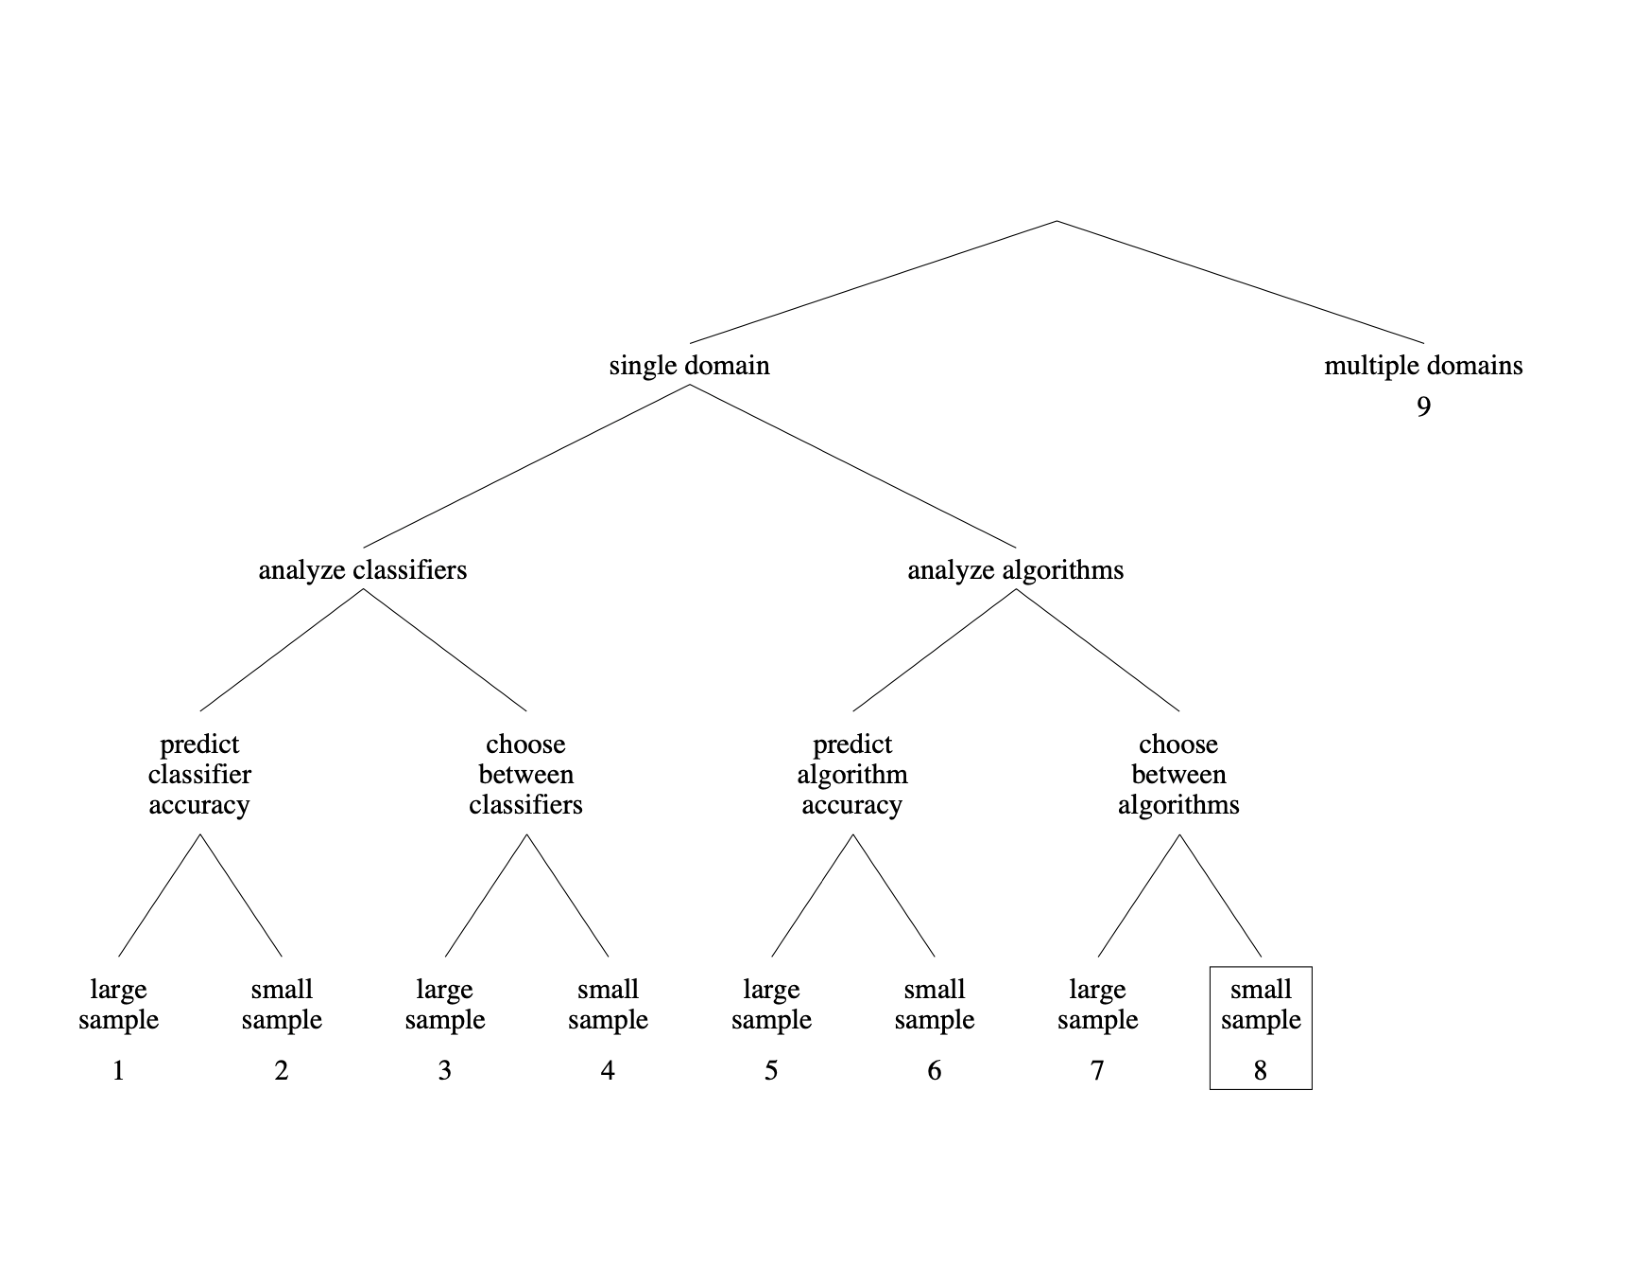
\includegraphics[scale=.5]{TaxonomicalQuestion.pdf} 

El siguiente nivel distingue entre estimar la precisi\'on y elegir clasificadores o algoritmos. El nivel m\'as bajo est\'a relacionado con la cantidad de datos disponibles, si se tiene una gran cantidad de datos, entonces se pueden fijar un conjunto de ellos para ser considerados como datos de prueba para evaluar los clasificadores. En muchos de los casos, la cantidad de datos es limitada y se requeire utilizar todos como datos de entrada a los algoritmos de aprendizaje, esto quiere decir que se requiere utilizar algunas t\'ecnicas de remuestreo para realizar an\'alisis estad\'isticos.

\begin{Note}\textbf{Nueve Preguntas}\\
Se supone que todos los puntos de datos se obtienen de manrea independiente de una distribuci\'on de probabilidad fija definida por el problema en particular.
\begin{Quest}
Sup\'ongase que se tiene una muestra de datos grande y un clasificador $C$. El clasificador pudo haber sido construido utilizando parte de los datos, pero a\'un existen datos para conformar un conjunto de datos de prueba. Por tanto se puede medir la precisi\'on de $C$ en el conjunto de datos de prueba y construir un intervalo de confianza binomial. El clasificador pudo haber sido generado por cualquier m\'etodo y no necesariamente por un algoritmo de aprendizaje.
\end{Quest}

\begin{Quest}
Dado un conjunto de datos peque\~no $S$, sup\'ongase que se aplica un algoritmo de aprendizaje $A$ a $S$ para construir un clasificador $C_{A}$, qu\'e tan preciso es el clasificador $C_A$ para nuevos ejemplos. Dado que no se tienen conjuntos de datos separados no es posible responder la pregunta directamente. Es posible predecir la precisi\'on del algoritmo $A$ cuando se entrena en conjuntos de datos seleccionados aleatoriamente de aproximadamente el mismo tama\~no que $S$. Si esto es posible entonces se puede predecir la precisi\'on de $C_A$ que fue obtenido  despues de ser entrenado en $S$. 

\end{Quest}


\begin{Quest}
Dados dos clasificadores $C_A$ y $C_B$ y suficientes datos para tener un conjunto de datos de prueba, determinar cual clasificador ser\'a m\'as preciso en nuevos ejemplos de prueba.  Esto se puede responder midiendo la precisi\'on de cada clasificador en los datos de prueba y aplicando la prueba de McNemar.

\end{Quest}


\begin{Quest}


\end{Quest}


\begin{Quest}


\end{Quest}


\begin{Quest}


\end{Quest}


\begin{Quest}


\end{Quest}


\begin{Quest}


\end{Quest}


\begin{Quest}


\end{Quest}

\end{Note}



\newpage


\section{Guia de estudio de Machine Learning}

\begin{itemize}
    \item Algoritmos de aprendizaje supervisado:
        \begin{itemize}
            \item Regresión lineal y logística
            \item Máquinas de soporte vectorial (SVM)
            \item Árboles de decisión y bosques aleatorios
            \item Redes neuronales
        \end{itemize}
    \item Aprendizaje no supervisado:
        \begin{itemize}
            \item K-Means y clustering jerárquico
            \item Análisis de componentes principales (PCA)
            \item Algoritmos de asociación
            \item Mapas autoorganizados (SOM)
        \end{itemize}
    \item Evaluación de modelos y métricas:
        \begin{itemize}
            \item Precisión, sensibilidad, especificidad
            \item Curvas ROC y área bajo la curva (AUC-ROC)
            \item Matriz de confusión
            \item Validación cruzada
        \end{itemize}
    \item Preprocesamiento de datos:
        \begin{itemize}
            \item Normalización y estandarización
            \item Manejo de datos faltantes
            \item Ingeniería de características
            \item Selección de características
        \end{itemize}
    \item Optimización de modelos:
        \begin{itemize}
            \item Hiperparámetros y búsqueda en cuadrícula
            \item Optimización bayesiana
            \item Regularización
            \item Redes neuronales convolucionales (CNN) y recurrentes (RNN)
        \end{itemize}
    \item Aprendizaje por refuerzo:
        \begin{itemize}
            \item Q-Learning
            \item Algoritmos de políticas
            \item Exploración y explotación
            \item Funciones de valor
        \end{itemize}
    \item Ética en el machine learning:
        \begin{itemize}
            \item Sesgo y equidad
            \item Transparencia y explicabilidad
            \item Privacidad y seguridad
            \item Responsabilidad en el despliegue de modelos
        \end{itemize}
\end{itemize}


\subsection{SVM}

\begin{enumerate}
    \item \textbf{Hiperplano:}
        En un espacio de características $n$-dimensional, un hiperplano es un subespacio de dimensión $n-1$. Para un problema de clasificación binaria, un hiperplano divide el espacio en dos regiones, asignando puntos a una clase u otra.

    \item \textbf{Margen:}
        El margen es la distancia perpendicular desde el hiperplano a los puntos más cercanos de cada clase. SVM busca el hiperplano que maximiza este margen, lo que se traduce en una mayor robustez y generalización del modelo.

    \item \textbf{Vectores de Soporte:}
        Estos son los puntos de datos más cercanos al hiperplano y tienen un papel crucial en la definición del margen. Cambiar estos vectores de soporte afecta directamente al modelo, y son los únicos puntos que importan para la determinación del hiperplano.

    \item \textbf{Función de Decisión:}
        La función de decisión de SVM es el hiperplano que se utiliza para clasificar nuevos puntos de datos. Dada una entrada, la función de decisión evalúa de qué lado del hiperplano cae el punto y asigna la etiqueta correspondiente.

    \item \textbf{Kernel Trick:}
        SVM puede manejar eficientemente datos no lineales mediante el uso de funciones de kernel. Estas funciones transforman el espacio de características original en uno de mayor dimensión, permitiendo así que los datos sean separados de manera no lineal en el espacio transformado.

    \item \textbf{Parámetros de SVM:}
        \begin{itemize}
            \item \textbf{C (Parámetro de Regularización):} Controla el equilibrio entre tener un margen más amplio y clasificar correctamente los puntos de entrenamiento.
            \item \textbf{Kernel:} Define la función de kernel utilizada (lineal, polinómica, radial, etc.).
            \item \textbf{Gamma (para kernels no lineales):} Controla el alcance de influencia de un solo punto de datos en la decisión.
        \end{itemize}

    \item \textbf{Proceso de Entrenamiento:}
        Dado un conjunto de datos de entrenamiento etiquetado, SVM busca el hiperplano óptimo que maximiza el margen entre las clases. Esto se realiza a través de técnicas de optimización cuadrática.

    \item \textbf{SVM para Regresión:}
        Además de la clasificación, SVM se puede utilizar para problemas de regresión. En este caso, el objetivo es ajustar un hiperplano de modo que contenga la mayor cantidad posible de puntos dentro de un margen predefinido.

    \item \textbf{Ventajas y Desventajas:}
        \begin{itemize}
            \item \textbf{Ventajas:} Efectivo en espacios de alta dimensión, eficaz en conjuntos de datos pequeños y versátil gracias al kernel trick.
            \item \textbf{Desventajas:} Sensible a la escala de las características, puede ser computacionalmente costoso para grandes conjuntos de datos y requiere la elección cuidadosa de parámetros.
        \end{itemize}

    \item \textbf{Aplicaciones:}
        SVM se utiliza en una variedad de campos, como reconocimiento de escritura, clasificación de imágenes, diagnóstico médico, entre otros.

\end{enumerate}


\subsubsection{Elementos Matemáticos de las SVM}

\begin{enumerate}
    \item \textbf{Hiperplano:}
        Un hiperplano se define como \(w \cdot x - b = 0\), donde \(w\) es el vector de pesos, \(x\) es el vector de entrada, y \(b\) es el sesgo.

    \item \textbf{Margen:}
        El margen \(M\) entre un hiperplano y un punto \(x_i\) se define como \(M = \frac{1}{\|w\|} |w \cdot x_i - b|\).

    \item \textbf{Vectores de Soporte:}
        Los vectores de soporte son los puntos \(x_i\) que cumplen la condición \(|w \cdot x_i - b| = 1/\|w\|\).

    \item \textbf{Función de Decisión:}
        La función de decisión es \(f(x) = w \cdot x - b\). Si \(f(x) > 0\), el punto \(x\) se clasifica como clase 1; si \(f(x) < 0\), se clasifica como clase -1.

    \item \textbf{Kernel Trick:}
        La función de kernel \(K(x, x')\) representa el producto escalar en un espacio de características de mayor dimensión. Ejemplos comunes incluyen el kernel lineal (\(K(x, x') = x \cdot x'\)), kernel polinómico (\(K(x, x') = (x \cdot x' + 1)^d\)), y kernel radial (\(K(x, x') = \exp(-\gamma \|x - x'\|^2)\)).

    \item \textbf{Parámetros de SVM:}
        \begin{itemize}
            \item \(C\) (Parámetro de Regularización): Se introduce en la función de pérdida para controlar el equilibrio entre tener un margen más amplio y clasificar correctamente los puntos de entrenamiento.
            \item \(w\) (Vector de Pesos): Aprende durante el entrenamiento y define la orientación del hiperplano.
            \item \(b\) (Sesgo): Parámetro de ajuste del hiperplano.
            \item \(\gamma\) (para kernels no lineales): Controla el alcance de influencia de un solo punto de datos en la decisión.
        \end{itemize}

    \item \textbf{Proceso de Entrenamiento:}
        El proceso de entrenamiento implica la minimización de la función de pérdida, que incluye el término de regularización \(C\|w\|^2\) y la función de pérdida hinge.

    \item \textbf{SVM para Regresión:}
        Para regresión, el objetivo es ajustar un hiperplano de modo que \(|w \cdot x_i - b| \leq \epsilon\) para puntos de entrenamiento \(x_i\).

    \item \textbf{Ventajas y Desventajas:}
        \begin{itemize}
            \item Ventajas: Efectivo en espacios de alta dimensión, eficaz en conjuntos de datos pequeños y versátil gracias al kernel trick.
            \item Desventajas: Sensible a la escala de las características, puede ser computacionalmente costoso para grandes conjuntos de datos y requiere la elección cuidadosa de parámetros.
        \end{itemize}

    \item \textbf{Aplicaciones:}
        SVM se aplica en una variedad de problemas, como reconocimiento de escritura, clasificación de imágenes y diagnóstico médico.
\end{enumerate}


\subsection{Árboles de Decisión}

\begin{enumerate}
    \item \textbf{Definición:}
        Un árbol de decisión es una estructura jerárquica en forma de árbol que se utiliza para representar decisiones y sus posibles consecuencias. Cada nodo interno del árbol representa una prueba en una característica, cada rama representa un resultado posible de la prueba, y cada hoja representa un resultado final o una decisión.

    \item \textbf{Proceso de Construcción:}
        El árbol se construye de manera recursiva. En cada paso, se elige la mejor característica para dividir el conjunto de datos en función de algún criterio, como la ganancia de información o la impureza de Gini. Este proceso se repite hasta que se alcanza algún criterio de parada, como la profundidad máxima del árbol o un número mínimo de puntos en una hoja.

    \item \textbf{Criterios de División:}
        Los criterios comunes para la división incluyen:
        \begin{itemize}
            \item \textbf{Ganancia de Información:} Mide cuánta información nueva proporciona una característica.
            \item \textbf{Impureza de Gini:} Mide la probabilidad de clasificar incorrectamente un elemento si es etiquetado aleatoriamente.
        \end{itemize}

    \item \textbf{Ventajas y Desventajas:}
        \begin{itemize}
            \item \textbf{Ventajas:} Fácil interpretación, no requiere normalización de datos, manejo natural de características categóricas.
            \item \textbf{Desventajas:} Propenso al sobreajuste, especialmente en conjuntos de datos pequeños y ruidosos.
        \end{itemize}
\end{enumerate}

\subsubsection{Bosques Aleatorios}

\begin{enumerate}
    \item \textbf{Definición:}
        Un bosque aleatorio es una colección de árboles de decisión entrenados en subconjuntos aleatorios del conjunto de datos y utilizando técnicas de agregación para mejorar la precisión y controlar el sobreajuste.

    \item \textbf{Proceso de Construcción:}
        Se crean múltiples árboles de decisión utilizando diferentes subconjuntos del conjunto de datos de entrenamiento y características aleatorias en cada división. Luego, las predicciones de cada árbol se promedian (en regresión) o se votan (en clasificación) para obtener la predicción final del bosque.

    \item \textbf{Técnica de Bagging:}
        La construcción de árboles en subconjuntos aleatorios del conjunto de datos se conoce como bagging (bootstrap aggregating). Esto ayuda a reducir la varianza y evitar el sobreajuste al promediar los errores.

    \item \textbf{Importancia de Características:}
        Los bosques aleatorios proporcionan una medida de la importancia de las características, que indica cuánto contribuye cada característica a la precisión del modelo. Esto es útil para la selección de características.

    \item \textbf{Ventajas y Desventajas:}
        \begin{itemize}
            \item \textbf{Ventajas:} Reducción del sobreajuste en comparación con un solo árbol, manejo automático del sobreajuste, buen rendimiento en conjuntos de datos grandes y complejos.
            \item \textbf{Desventajas:} Menos interpretables que los árboles de decisión individuales.
        \end{itemize}
\end{enumerate}

\subsubsection{Elementos Matemáticos de Árboles de Decisión}

\begin{enumerate}
    \item \textbf{Definición:}
        Un árbol de decisión se representa como una función \(T(x)\) que asigna una instancia \(x\) a una hoja del árbol. Cada nodo interno \(j\) realiza una prueba en una característica \(f_j(x)\), y cada rama representa una condición de prueba. La estructura del árbol se define por las funciones indicadoras \(I(x, j)\) que indican si la instancia \(x\) llega al nodo \(j\).
        
        \[ T(x) = \sum_{j=1}^{J} I(x, j) \cdot C_j \]

        Donde \(J\) es el número de nodos, \(C_j\) es el valor en la hoja correspondiente al nodo \(j\), y \(I(x, j)\) es 1 si la instancia \(x\) llega al nodo \(j\) y 0 de lo contrario.

    \item \textbf{Proceso de Construcción:}
        La construcción del árbol implica seleccionar la mejor característica \(f_j\) y el umbral \(t_j\) en cada nodo \(j\) para maximizar la ganancia de información o reducir la impureza de Gini.
        
        \[ \textrm{Ganancia de Información: } Gain(D, j, t) = H(D) - \frac{N_L}{N} H(D_L) - \frac{N_R}{N} H(D_R) \]

        \[ \textrm{Impureza de Gini: } Gini(D) = 1 - \sum_{k=1}^{K} \left(\frac{|C_k|}{|D|}\right)^2 \]

        Donde \(D\) es el conjunto de datos en el nodo, \(D_L\) y \(D_R\) son los conjuntos de datos en los nodos izquierdo y derecho después de la división, \(N\) es el número total de instancias en \(D\), y \(N_L\) y \(N_R\) son los números de instancias en los nodos izquierdo y derecho.

    \item \textbf{Ventajas y Desventajas:}
        \begin{itemize}
            \item \textbf{Ventajas:} Fácil interpretación, no requiere normalización de datos, manejo natural de características categóricas.
            \item \textbf{Desventajas:} Propenso al sobreajuste, especialmente en conjuntos de datos pequeños y ruidosos.
        \end{itemize}
\end{enumerate}

\subsubsection{Bosques Aleatorios}

\begin{enumerate}
    \item \textbf{Definición:}
        Un bosque aleatorio es una colección de \(B\) árboles de decisión \(T_b(x)\), donde cada árbol se entrena en un subconjunto aleatorio de los datos de entrenamiento. La predicción se obtiene promediando (en regresión) o votando (en clasificación) las predicciones individuales de los árboles.

        \[ \textrm{Predicción del Bosque: } \hat{Y}(x) = \frac{1}{B} \sum_{b=1}^{B} T_b(x) \]

    \item \textbf{Proceso de Construcción:}
        Cada árbol en el bosque se construye utilizando bagging, que consiste en seleccionar aleatoriamente un subconjunto de las instancias de entrenamiento con reemplazo. Además, en cada división de nodo, se selecciona un subconjunto aleatorio de características.

        \[ \textrm{Bagging: } D_b = \{(x_i, y_i)\} \textrm{ con } i \sim \textrm{Uniforme}(1, N) \]

        \[ \textrm{Características Aleatorias: } f_j \textrm{ con } j \sim \textrm{Uniforme}(1, P) \]

    \item \textbf{Importancia de Características:}
        La importancia de la característica \(f_j\) se mide mediante la disminución promedio en la ganancia de impureza o la reducción en el error cuadrático medio cuando se utiliza \(f_j\) para dividir los nodos a lo largo de todos los árboles.

        \[ \textrm{Importancia de } f_j = \frac{1}{B} \sum_{b=1}^{B} \sum_{j \textrm{ en } T_b} \textrm{Importancia de } f_j \textrm{ en } T_b \]

\end{enumerate}








\section{Referencias}
\begin{itemize}
    \item Libros:
        \begin{enumerate}
            \item "The Hundred-Page Machine Learning Book" por Andriy Burkov
            \item "Machine Learning: A Probabilistic Perspective" por Kevin P. Murphy
            \item "Hands-On Machine Learning with Scikit-Learn, Keras, and TensorFlow" por Aurélien Géron
            \item "Pattern Recognition and Machine Learning" por Christopher M. Bishop
            \item "Deep Learning" por Ian Goodfellow, Yoshua Bengio y Aaron Courville
        \end{enumerate}
    \item Cursos:
        \begin{enumerate}
            \item "Machine Learning" por Andrew Ng en Coursera
            \item "Applied Data Science with Python" por la Universidad de Míchigan en Coursera
            \item "Deep Learning Specialization" por Andrew Ng en Coursera
            \item "Machine Learning Crash Course" por Google
            \item "Introduction to Machine Learning" por la Universidad de Columbia en edX
        \end{enumerate}
    \item Sitios web:
        \begin{enumerate}
            \item Kaggle
            \item GitHub
            \item Towards Data Science
            \item Machine Learning Mastery
            \item Google AI
        \end{enumerate}
\end{itemize}


Fuentes:
\begin{enumerate}
    \item Machine Learning citation style [Update October 2023] - Paperpile
    \item ICML2021 Template - Overleaf, Online LaTeX Editor
    \item Machine Learning | Submission guidelines - Springer
    \item Journal of Machine Learning Research
\end{enumerate}

%== == ==  == == == ==  == == == ==  == == == ==  == == == ==  == 
\section{Bioinformatics: New revision}
%== == ==  == == == ==  == == == ==  == == == ==  == == == ==  == 

%-- -- -- -- -- -- -- -- -- -- -- -- -- -- -- -- -- -- -- -- -- -- -- -- -- -- -- -- -- -- 
\subsection{A bayesian framework for combining gene predictions - Pavlovic}
%-- -- -- -- -- -- -- -- -- -- -- -- -- -- -- -- -- -- -- -- -- -- -- -- -- -- -- -- -- -- 

Biology and biotechnology are undergoing a techonolgical revolution which is transforming research into an information-rich enterprise.  A typical bacterial genome sequence is comprised of several million bases of DNA and contains several thousand genes. The human genome is approximately 3 billion bases long and it contains approximately 30,000 putative genes identified thus far.



%== == ==  == == == ==  == == == ==  == == == ==  == == == ==  == 
\section{Random Forest: Explanation in Mathematical Terms}

Random Forest is a supervised learning algorithm used for both classification and regression problems. The main idea behind Random Forest is to build multiple decision trees during training and combine their results to obtain a more robust and accurate prediction.

Let's assume we have a training dataset \(D = \{(x_1, y_1), (x_2, y_2), \ldots, (x_n, y_n)\}\), where \(x_i\) represents the features and \(y_i\) is the target variable.

\begin{enumerate}
    \item \textbf{Construction of Decision Trees:}
        \begin{itemize}
            \item For each tree, a random subset of features is selected (randomly sample features), and a random subset of training data is chosen (randomly sample observations with replacement).
            \item A decision tree is constructed using the subset of data and features.
            \item The decision tree is represented as \(h_i(x;\theta_i)\), where \(i\) denotes the tree index, \(x\) is the input feature vector, and \(\theta_i\) represents the parameters of the tree.
            \item At each node \(t\) of the tree, a feature \(j_t\) is selected from the random subset, and the split is determined based on minimizing impurity:
            \[
            \theta_{i,t} = \arg\min_{j_t, s_t} \left[\textrm{Impurity}(D_t) - p_{\textrm{left}}\textrm{Impurity}(D_{\textrm{left}}) - p_{\textrm{right}}\textrm{Impurity}(D_{\textrm{right}})\right]
            \]
            where \(D_t\) is the dataset at node \(t\), \(D_{\textrm{left}}\) and \(D_{\textrm{right}}\) are the datasets in the left and right child nodes, \(p_{\textrm{left}}\) and \(p_{\textrm{right}}\) are the proportions of data in the left and right child nodes, and \(\textrm{Impurity}(\cdot)\) is a measure of impurity, such as Gini index for classification or mean squared error for regression.
        \end{itemize}
    
    \item \textbf{Voting or Averaging:}
        \begin{itemize}
            \item For classification problems, the final prediction is obtained by majority voting among the trees:
            \[
            H(x) = \textrm{mode}\{h_1(x;\theta_1), h_2(x;\theta_2), \ldots, h_n(x;\theta_n)\}
            \]
            \item For regression problems, the final prediction is the average of predictions from all trees:
            \[
            H(x) = \frac{1}{n}\sum_{i=1}^{n}h_i(x;\theta_i)
            \]
        \end{itemize}
    
    \item \textbf{Variance Reduction:}
        \begin{itemize}
            \item By building decision trees in a random manner, the variance of the model is reduced, leading to a more robust and generalizable model.
        \end{itemize}
\end{enumerate}

The final prediction is obtained by combining the predictions of all trees.

\section{Deep Learning: Overview}

Deep Learning is a subfield of machine learning that focuses on neural networks with multiple layers (deep neural networks). These networks can automatically learn hierarchical representations of data, allowing them to capture intricate patterns and features.

\begin{enumerate}
    \item \textbf{Neural Network Representation:}
        \begin{itemize}
            \item A neural network consists of layers of interconnected nodes (neurons) organized into an input layer, one or more hidden layers, and an output layer.
            \item The input layer represents the features of the data, and each neuron in the layer processes a specific feature.
            \item Hidden layers perform nonlinear transformations on the input data, learning hierarchical representations.
            \item The output layer produces the final prediction based on the learned representations.
        \end{itemize}
    
    \item \textbf{Training a Neural Network:}
        \begin{itemize}
            \item During training, the network's parameters (weights and biases) are adjusted to minimize the difference between predicted and actual outputs.
            \item This optimization is typically done using backpropagation and gradient descent.
        \end{itemize}
    
    \item \textbf{Activation Functions:}
        \begin{itemize}
            \item Activation functions introduce nonlinearity to the neural network, enabling it to learn complex patterns.
            \item Common activation functions include ReLU (Rectified Linear Unit), Sigmoid, and Hyperbolic Tangent (tanh).
        \end{itemize}
    
    \item \textbf{Forward Pass:}
        \begin{itemize}
            \item The forward pass of a neural network involves computing the output of the network for a given input.
            \item Given an input vector \(x\), the output \(y\) is computed by passing \(x\) through the network's layers using learned weights and biases.
            \item The output of each layer is computed as:
            \[
            a^{(l)} = W^{(l)}a^{(l-1)} + b^{(l)}
            \]
            where \(W^{(l)}\) is the weight matrix, \(a^{(l)}\) is the activation of layer \(l\), \(a^{(l-1)}\) is the activation of the previous layer, and \(b^{(l)}\) is the bias vector.
            \item The activation function is then applied to \(a^{(l)}\) to introduce nonlinearity.
        \end{itemize}
    
    \item \textbf{Loss Function:}
        \begin{itemize}
            \item The loss function measures the difference between the predicted output and the true output.
            \item Common loss functions include mean squared error for regression and cross-entropy for classification.
            \item The goal during training is to minimize the loss by adjusting the network's parameters.
        \end{itemize}
    
    \item \textbf{Backpropagation:}
        \begin{itemize}
            \item Backpropagation is a training algorithm that computes the gradient of the loss with respect to the network's parameters.
            \item The gradient is used to update the parameters in the direction that reduces the loss.
            \item It involves computing the gradient of the loss with respect to the output of each layer and using the chain rule to propagate these gradients backward through the network.
        \end{itemize}
\end{enumerate}

\section{Example of Implementation in R:}

\subsection{Install and Load the Keras Library:}
\begin{verbatim}
install.packages("keras")
library(keras)
\end{verbatim}

\subsection{Build a Simple Neural Network:}
\begin{verbatim}
model <- keras_model_sequential() %>%
  layer_dense(units = 128, activation = 'relu', input_shape = c(10)) %>%
  layer_dense(units = 1, activation = 'sigmoid')

summary(model)
\end{verbatim}

\subsection{Compile and Train the Neural Network:}
\begin{verbatim}
model %>% compile(
  optimizer = 'adam',
  loss = 'binary_crossentropy',
  metrics = c('accuracy')
)

# Assuming you have training data X_train and labels y_train
history <- model %>% fit(
  X_train, y_train,
  epochs = 10, batch_size = 32,
  validation_split = 0.2
)
\end{verbatim}

\subsection{Evaluate the Model:}
\begin{verbatim}
# Assuming you have test data X_test and labels y_test
evaluate_result <- model %>% evaluate(X_test, y_test)
print(evaluate_result)
\end{verbatim}


\section{Impurity Measures in Random Forest}

In the context of Random Forest, impurity measures play a crucial role in the construction of decision trees. The two commonly used impurity measures are the Gini index for classification and the mean squared error for regression.

\subsection{Gini Index for Classification}

The Gini index is a measure of impurity used in classification problems. Given a node in a decision tree that contains data points from different classes, the Gini index quantifies how often a randomly chosen data point would be incorrectly classified.

For a node \(t\) with \(K\) classes and a set of data points \(D_t\), the Gini index (\(Gini(t)\)) is calculated as follows:

\[ Gini(t) = 1 - \sum_{i=1}^{K} p_i^2 \]

where \(p_i\) is the proportion of data points in class \(i\) at node \(t\). A lower Gini index indicates a purer node with predominantly one class.

In the context of Random Forest, the decision tree split is determined by minimizing the weighted sum of Gini indices for the left and right child nodes. The split that results in the lowest overall Gini index is chosen.

\subsection{Mean Squared Error for Regression}

For regression problems, the impurity measure used is the mean squared error (MSE). Unlike classification, where impurity is related to the purity of classes in a node, regression impurity is a measure of the variability of target values within a node.

For a node \(t\) with data points \(D_t\), the MSE (\(MSE(t)\)) is calculated as follows:

\[ MSE(t) = \frac{1}{|D_t|} \sum_{i \in D_t} (y_i - \bar{y}_t)^2 \]

where \(y_i\) is the target value of data point \(i\), \(|D_t|\) is the number of data points in node \(t\), and \(\bar{y}_t\) is the mean target value of all data points in node \(t\).

Similar to the Gini index, in Random Forest, the decision tree split is determined by minimizing the weighted sum of MSE for the left and right child nodes.

These impurity measures guide the construction of individual decision trees within the Random Forest ensemble, contributing to the overall robustness and predictive power of the model.


\section{Construcción del Árbol de Decisión}

\subsection{Teoría:}

Un árbol de decisión es una estructura de datos que representa un conjunto de decisiones y sus posibles consecuencias. En el contexto de Random Forest, la construcción de un árbol de decisión sigue el principio de "aprendizaje supervisado", donde el algoritmo aprende patrones a partir de un conjunto de datos etiquetado.

La construcción del árbol se realiza a través de divisiones recursivas basadas en características del conjunto de datos. Cada nodo del árbol representa una pregunta sobre una característica, y las ramas que surgen de ese nodo son las respuestas a esa pregunta. El proceso continúa hasta que se alcanza un criterio de parada, como la profundidad máxima del árbol o el número mínimo de muestras en un nodo.

\subsection{Elementos Matemáticos:}

1. \textbf{Función de Impureza:}

En cada nodo del árbol, se elige la característica y el umbral que minimizan la impureza en los nodos hijos resultantes. La impureza se mide mediante funciones como el Índice de Gini para clasificación o el Error Cuadrático Medio (MSE) para regresión.

Para clasificación:
\[ Gini(t) = 1 - \sum_{i=1}^{K} p_i^2 \]

Donde \( p_i \) es la proporción de ejemplos de la clase \( i \) en el nodo \( t \).

Para regresión:
\[ MSE(t) = \frac{1}{|D_t|} \sum_{i \in D_t} (y_i - \bar{y}_t)^2 \]

Donde \( D_t \) es el conjunto de datos en el nodo \( t \), \( y_i \) es la etiqueta del ejemplo \( i \), y \( \bar{y}_t \) es la media de las etiquetas en el nodo \( t \).

2. \textbf{Criterio de División:}

La elección de la mejor característica y umbral se basa en la reducción de la impureza. Se busca el par \((j, s)\) que minimiza la expresión:
\[ \theta_{i,t} = \arg\min_{j, s} \left[ \textrm{Impureza}(D_t) - p_{\textrm{left}}\textrm{Impureza}(D_{\textrm{left}}) - p_{\textrm{right}}\textrm{Impureza}(D_{\textrm{right}}) \right] \]

Donde \(D_t\) es el conjunto de datos en el nodo \(t\), \(D_{\textrm{left}}\) y \(D_{\textrm{right}}\) son los conjuntos de datos en los nodos izquierdo y derecho después de la división, y \(p_{\textrm{left}}\) y \(p_{\textrm{right}}\) son las proporciones de datos en esos nodos.

3. \textbf{Criterios de Parada:}

Para evitar sobreajuste, se utilizan criterios de parada, como la profundidad máxima del árbol o el número mínimo de muestras requeridas para realizar una división.

La construcción de cada árbol en Random Forest implica este proceso iterativo y se repite para cada árbol en el bosque. La diversidad en la construcción de árboles se logra mediante el uso de diferentes subconjuntos aleatorios de características y datos en cada árbol. La combinación de predicciones de estos árboles mejora la generalización del modelo y su capacidad predictiva en nuevos datos.



\section{Reducción de Varianza en Random Forest}

\subsection{Teoría:}

La reducción de la varianza es uno de los objetivos clave en la construcción de árboles de decisión en Random Forest. Esta técnica busca mejorar la generalización del modelo al reducir la sensibilidad a pequeñas variaciones en los datos de entrenamiento.

La varianza se refiere a la variabilidad de las predicciones de un modelo respecto a diferentes conjuntos de datos de entrenamiento. En Random Forest, la reducción de la varianza se logra mediante dos técnicas principales: Bagging y Random Subspace.

\subsubsection{Bagging (Bootstrap Aggregating):}

Bagging es una técnica que consiste en entrenar múltiples modelos en diferentes subconjuntos de datos generados mediante muestreo con reemplazo (bootstrap). Cada árbol de decisión en Random Forest se entrena en un conjunto de datos ligeramente diferente, lo que introduce diversidad en los modelos.

\subsubsection{Random Subspace:}

Random Subspace es otra técnica utilizada para reducir la correlación entre los árboles de decisión. En lugar de usar todas las características para cada árbol, se selecciona un subconjunto aleatorio de características para entrenar cada árbol. Esto ayuda a que cada árbol se especialice en diferentes aspectos de los datos, mejorando la diversidad y reduciendo la correlación entre las predicciones.

\subsection{Elementos Matemáticos:}

La reducción de la varianza no se expresa directamente con fórmulas matemáticas específicas, pero los conceptos clave son fundamentales:

1. **Bagging:**
    - Cada árbol \(T_i\) se entrena en un conjunto de datos \(D_i\) generado por muestreo con reemplazo (bootstrap).
    - La predicción final se obtiene promediando las predicciones de todos los árboles:
        \[ H(x) = \frac{1}{N} \sum_{i=1}^{N} T_i(x) \]

2. **Random Subspace:**
    - Cada árbol \(T_i\) se entrena utilizando un subconjunto aleatorio de características.
    - La predicción final se obtiene promediando las predicciones de todos los árboles:
        \[ H(x) = \frac{1}{N} \sum_{i=1}^{N} T_i(x) \]

Estos enfoques combinados contribuyen a reducir la varianza del modelo, lo que resulta en un modelo más robusto y generalizable.

\section{Votación y Promedio en Random Forest}

\subsection{Teoría:}

La técnica de "Votación" (para problemas de clasificación) o "Promedio" (para problemas de regresión) es crucial en Random Forest para combinar las predicciones de múltiples árboles de decisión y obtener una predicción final más robusta y precisa.

\subsubsection{Para Problemas de Clasificación:}

En problemas de clasificación, el enfoque de votación se utiliza. Cada árbol en el bosque emite una predicción de clase, y la clase final se determina por mayoría de votos.

\subsubsection{Para Problemas de Regresión:}

En problemas de regresión, se utiliza un enfoque de promedio. Cada árbol realiza una predicción numérica, y la predicción final es el promedio de todas las predicciones.

\subsection{Elementos Matemáticos:}

1. \textbf{Votación para Clasificación:}
    - La predicción final para un ejemplo \(x\) se obtiene por mayoría de votos:
        \[ H(x) = \textrm{mode}\{T_1(x), T_2(x), ..., T_N(x)\} \]

2. \textbf{Promedio para Regresión:}
    - La predicción final para un ejemplo \(x\) se obtiene promediando las predicciones de todos los árboles:
        \[ H(x) = \frac{1}{N}\sum_{i=1}^{N} T_i(x) \]

Donde \(T_i(x)\) representa la predicción del árbol \(i\) para el ejemplo \(x\), y \(N\) es el número total de árboles en el bosque.

Estos enfoques de votación y promedio permiten que Random Forest combine la información de múltiples árboles de decisión, mejorando la generalización y la capacidad predictiva del modelo.

\section{Resumen}

Random Forest es un algoritmo de aprendizaje automático que se utiliza para resolver problemas de clasificación y regresión. En lugar de utilizar un único árbol de decisión, Random Forest construye varios árboles de decisión y los combina para obtener una predicción más precisa. Cada árbol de decisión se construye utilizando un subconjunto aleatorio de las características del conjunto de datos original. Al final, las predicciones de cada árbol se promedian para obtener una predicción final.

El algoritmo de Random Forest se basa en dos técnicas: Bagging y Random Subspace. Bagging es una técnica que se utiliza para reducir la varianza de un modelo al entrenar múltiples modelos en diferentes subconjuntos de datos. Random Subspace es una técnica que se utiliza para reducir la correlación entre los modelos al entrenar cada modelo en diferentes subconjuntos de características.

Aquí hay algunos elementos matemáticos que se utilizan en Random Forest:

\begin{itemize}
    \item \textbf{Árbol de decisión:} Un árbol de decisión es una estructura de datos que se utiliza para modelar decisiones y sus posibles consecuencias. Cada nodo en el árbol representa una decisión, y cada rama representa una posible consecuencia de esa decisión. Los árboles de decisión se construyen utilizando un conjunto de reglas que se utilizan para tomar decisiones.
    \item \textbf{Bootstrap:} Bootstrap es una técnica que se utiliza para generar múltiples conjuntos de datos a partir de un conjunto de datos original. Cada conjunto de datos se genera mediante muestreo con reemplazo, lo que significa que cada elemento del conjunto de datos original tiene la misma probabilidad de ser seleccionado en cada conjunto de datos generado.
    \item \textbf{Out-of-Bag Error:} Out-of-Bag Error es una técnica que se utiliza para estimar el error de validación de un modelo sin la necesidad de un conjunto de datos de validación separado. El error se estima utilizando los datos que no se incluyeron en el conjunto de datos de entrenamiento para cada árbol de decisión.
\end{itemize}

\subsection{Ejemplo en R: Random Forest}

Aquí hay un ejemplo de cómo construir un modelo de bosque aleatorio en R:

\begin{verbatim}
# Cargamos el paquete necesario para este ejemplo
library(randomForest)

# Cargamos el conjunto de datos que deseamos utilizar
data(iris)

# Dividimos el conjunto de datos en conjuntos de entrenamiento y prueba
trainIndex <- createDataPartition(iris$Species, p = .8, list = FALSE, times = 1)

# Entrenamos el modelo de bosque aleatorio
rf_model <- randomForest(Species ~ ., data = iris[trainIndex,])

# Realizamos predicciones en el conjunto de prueba
predictions <- predict(rf_model, iris[-trainIndex,])
\end{verbatim}

\subsection{Deep Learning}

Deep Learning es un subcampo del aprendizaje automático que se centra en la creación de redes neuronales artificiales profundas. Estas redes neuronales están diseñadas para imitar el cerebro humano y son capaces de aprender patrones complejos en los datos.

Aquí hay un ejemplo de cómo construir una red neuronal profunda en R utilizando el paquete keras:

\begin{verbatim}
# Cargamos los paquetes necesarios
library(keras)
library(tensorflow)

# Cargamos el conjunto de datos que deseamos utilizar
data(iris)

# Dividimos el conjunto de datos en conjuntos de entrenamiento y prueba
trainIndex <- createDataPartition(iris$Species, p = .8, list = FALSE, times = 1)

# Creamos la red neuronal
model <- keras_model_sequential() %>% 
  layer_dense(units = 4, input_shape = c(4)) %>% 
  layer_activation("relu") %>% 
  layer_dense(units = 3) %>% 
  layer_activation("softmax")

# Compilamos la red neuronal
model %>% compile(loss = "categorical_crossentropy", optimizer = "adam", metrics = "accuracy")

# Entrenamos la red neuronal
history <- model %>% fit(
  x = iris[trainIndex, 1:4],
  y = to_categorical(as.numeric(iris[trainIndex, 5])),
  epochs = 100,
  batch_size = 10,
  validation_split = 0.2
)
\end{verbatim}



% ===_-_===_-_===_-_===_-_===_-_===_-_===
\section{Algoritmos de Aprendizaje Supervisado}
% ===_-_===_-_===_-_===_-_===_-_===_-_===

%__________________________________
\subsection{Regresión Lineal y Logística}
%__________________________________
    % Contenido sobre regresión lineal y logística
\subsubsection{Regresión Lineal}

La regresión lineal es un modelo que busca modelar la relación lineal entre una variable dependiente \(Y\) y una o más variables independientes \(X\). El modelo se define como:

\[
Y = \beta_0 + \beta_1 X + \varepsilon
\]

donde:
\begin{itemize}
    \item \(Y\) es la variable dependiente que queremos predecir.
    \item \(X\) es la variable independiente que utilizamos para la predicción.
    \item \(\beta_0\) es la ordenada al origen, que representa el valor de \(Y\) cuando \(X\) es cero.
    \item \(\beta_1\) es la pendiente de la recta, que indica cuánto cambia \(Y\) por un cambio unitario en \(X\).
    \item \(\varepsilon\) es el término de error que captura la variabilidad no explicada por el modelo.
\end{itemize}

El objetivo es encontrar los valores de \(\beta_0\) y \(\beta_1\) que minimizan la suma de los cuadrados de los errores \(\varepsilon\):

\[
\min_{\beta_0, \beta_1} \sum_{i=1}^{n} (Y_i - (\beta_0 + \beta_1 X_i))^2
\]

Esto se puede hacer utilizando técnicas como el método de mínimos cuadrados.

\subsubsection{Regresión Logística}

La regresión logística es un modelo utilizado para problemas de clasificación binaria. Se emplea la función logística, también conocida como la función sigmoide, para transformar la salida de la regresión lineal en un valor entre 0 y 1, que se interpreta como la probabilidad de pertenecer a la clase positiva. La función sigmoide está definida como:

\[
P(Y=1) = \frac{1}{1 + e^{-(\beta_0 + \beta_1 X)}}
\]

donde:
\begin{itemize}
    \item \(P(Y=1)\) es la probabilidad de pertenecer a la clase positiva.
    \item \(e\) es la base del logaritmo natural.
\end{itemize}

El modelo de regresión logística busca encontrar los valores de \(\beta_0\) y \(\beta_1\) que maximizan la función de verosimilitud. La función de verosimilitud es el producto de las probabilidades condicionales de observar las etiquetas de clase dados los valores de \(X\):

\[
\max_{\beta_0, \beta_1} \mathcal{L}(\beta_0, \beta_1) = \prod_{i=1}^{n} P(Y_i)^{y_i} \cdot (1 - P(Y_i))^{1 - y_i}
\]

donde:
\begin{itemize}
    \item \(\mathcal{L}(\beta_0, \beta_1)\) es la función de verosimilitud.
    \item \(y_i\) es la etiqueta de la clase para la observación \(i\).
\end{itemize}

La regresión logística se ajusta típicamente maximizando la log-verosimilitud para obtener estimaciones de \(\beta_0\) y \(\beta_1\).

\subsubsection{Implementacion}
\begin{verbatim}
# Ejemplo de Regresión Lineal
set.seed(123)
# Crear datos de ejemplo
X <- rnorm(100)
Y <- 2 * X + rnorm(100)

# Ajustar el modelo de regresión lineal
modelo_lineal <- lm(Y ~ X)

# Imprimir resultados
summary(modelo_lineal)

# Graficar el modelo
plot(X, Y, main = "Regresión Lineal", xlab = "X", ylab = "Y")
abline(modelo_lineal, col = "red")

# Ejemplo de Regresión Logística
set.seed(123)
# Crear datos de ejemplo para clasificación binaria
X <- rnorm(100)
probabilidades <- exp(2 * X) / (1 + exp(2 * X))
Y_binario <- rbinom(100, 1, probabilidades)

# Ajustar el modelo de regresión logística
modelo_logistico <- glm(Y_binario ~ X, family = binomial)

# Imprimir resultados
summary(modelo_logistico)

# Graficar el modelo
plot(X, Y_binario, main = "Regresión Logística", 
         xlab = "X", ylab = "Y", col = Y_binario + 1)
curve(predict(modelo_logistico, 
           data.frame(X = x), type = "response"), 
           add = TRUE, col = "red")
\end{verbatim}


%__________________________________
\subsection{Máquinas de Soporte Vectorial (SVM)}
%__________________________________
    % Contenido sobre SVM

\begin{enumerate}
    \item \textbf{Hiperplano:}
        En un espacio de características $n$-dimensional, un hiperplano es un subespacio de dimensión $n-1$. Para un problema de clasificación binaria, un hiperplano divide el espacio en dos regiones, asignando puntos a una clase u otra.

    \item \textbf{Margen:}
        El margen es la distancia perpendicular desde el hiperplano a los puntos más cercanos de cada clase. SVM busca el hiperplano que maximiza este margen, lo que se traduce en una mayor robustez y generalización del modelo.

    \item \textbf{Vectores de Soporte:}
        Estos son los puntos de datos más cercanos al hiperplano y tienen un papel crucial en la definición del margen. Cambiar estos vectores de soporte afecta directamente al modelo, y son los únicos puntos que importan para la determinación del hiperplano.

    \item \textbf{Función de Decisión:}
        La función de decisión de SVM es el hiperplano que se utiliza para clasificar nuevos puntos de datos. Dada una entrada, la función de decisión evalúa de qué lado del hiperplano cae el punto y asigna la etiqueta correspondiente.

    \item \textbf{Kernel Trick:}
        SVM puede manejar eficientemente datos no lineales mediante el uso de funciones de kernel. Estas funciones transforman el espacio de características original en uno de mayor dimensión, permitiendo así que los datos sean separados de manera no lineal en el espacio transformado.

    \item \textbf{Parámetros de SVM:}
        \begin{itemize}
            \item \textbf{C (Parámetro de Regularización):} Controla el equilibrio entre tener un margen más amplio y clasificar correctamente los puntos de entrenamiento.
            \item \textbf{Kernel:} Define la función de kernel utilizada (lineal, polinómica, radial, etc.).
            \item \textbf{Gamma (para kernels no lineales):} Controla el alcance de influencia de un solo punto de datos en la decisión.
        \end{itemize}

    \item \textbf{Proceso de Entrenamiento:}
        Dado un conjunto de datos de entrenamiento etiquetado, SVM busca el hiperplano óptimo que maximiza el margen entre las clases. Esto se realiza a través de técnicas de optimización cuadrática.

    \item \textbf{SVM para Regresión:}
        Además de la clasificación, SVM se puede utilizar para problemas de regresión. En este caso, el objetivo es ajustar un hiperplano de modo que contenga la mayor cantidad posible de puntos dentro de un margen predefinido.

    \item \textbf{Ventajas y Desventajas:}
        \begin{itemize}
            \item \textbf{Ventajas:} Efectivo en espacios de alta dimensión, eficaz en conjuntos de datos pequeños y versátil gracias al kernel trick.
            \item \textbf{Desventajas:} Sensible a la escala de las características, puede ser computacionalmente costoso para grandes conjuntos de datos y requiere la elección cuidadosa de parámetros.
        \end{itemize}

    \item \textbf{Aplicaciones:}
        SVM se utiliza en una variedad de campos, como reconocimiento de escritura, clasificación de imágenes, diagnóstico médico, entre otros.

\end{enumerate}


\subsubsection{Elementos Matemáticos de las SVM}

\begin{enumerate}
    \item \textbf{Hiperplano:}
        Un hiperplano se define como \(w \cdot x - b = 0\), donde \(w\) es el vector de pesos, \(x\) es el vector de entrada, y \(b\) es el sesgo.

    \item \textbf{Margen:}
        El margen \(M\) entre un hiperplano y un punto \(x_i\) se define como \(M = \frac{1}{\|w\|} |w \cdot x_i - b|\).

    \item \textbf{Vectores de Soporte:}
        Los vectores de soporte son los puntos \(x_i\) que cumplen la condición \(|w \cdot x_i - b| = 1/\|w\|\).

    \item \textbf{Función de Decisión:}
        La función de decisión es \(f(x) = w \cdot x - b\). Si \(f(x) > 0\), el punto \(x\) se clasifica como clase 1; si \(f(x) < 0\), se clasifica como clase -1.

    \item \textbf{Kernel Trick:}
        La función de kernel \(K(x, x')\) representa el producto escalar en un espacio de características de mayor dimensión. Ejemplos comunes incluyen el kernel lineal (\(K(x, x') = x \cdot x'\)), kernel polinómico (\(K(x, x') = (x \cdot x' + 1)^d\)), y kernel radial (\(K(x, x') = \exp(-\gamma \|x - x'\|^2)\)).

    \item \textbf{Parámetros de SVM:}
        \begin{itemize}
            \item \(C\) (Parámetro de Regularización): Se introduce en la función de pérdida para controlar el equilibrio entre tener un margen más amplio y clasificar correctamente los puntos de entrenamiento.
            \item \(w\) (Vector de Pesos): Aprende durante el entrenamiento y define la orientación del hiperplano.
            \item \(b\) (Sesgo): Parámetro de ajuste del hiperplano.
            \item \(\gamma\) (para kernels no lineales): Controla el alcance de influencia de un solo punto de datos en la decisión.
        \end{itemize}

    \item \textbf{Proceso de Entrenamiento:}
        El proceso de entrenamiento implica la minimización de la función de pérdida, que incluye el término de regularización \(C\|w\|^2\) y la función de pérdida hinge.

    \item \textbf{SVM para Regresión:}
        Para regresión, el objetivo es ajustar un hiperplano de modo que \(|w \cdot x_i - b| \leq \epsilon\) para puntos de entrenamiento \(x_i\).

    \item \textbf{Ventajas y Desventajas:}
        \begin{itemize}
            \item Ventajas: Efectivo en espacios de alta dimensión, eficaz en conjuntos de datos pequeños y versátil gracias al kernel trick.
            \item Desventajas: Sensible a la escala de las características, puede ser computacionalmente costoso para grandes conjuntos de datos y requiere la elección cuidadosa de parámetros.
        \end{itemize}

    \item \textbf{Aplicaciones:}
        SVM se aplica en una variedad de problemas, como reconocimiento de escritura, clasificación de imágenes y diagnóstico médico.
\end{enumerate}
    
    
  
%__________________________________
\subsection{Árboles de Decisión y Bosques Aleatorios}
%__________________________________
    % Contenido sobre árboles de decisión y bosques aleatorios
\begin{enumerate}
    \item \textbf{Definición:}
        Un árbol de decisión es una estructura jerárquica en forma de árbol que se utiliza para representar decisiones y sus posibles consecuencias. Cada nodo interno del árbol representa una prueba en una característica, cada rama representa un resultado posible de la prueba, y cada hoja representa un resultado final o una decisión.

    \item \textbf{Proceso de Construcción:}
        El árbol se construye de manera recursiva. En cada paso, se elige la mejor característica para dividir el conjunto de datos en función de algún criterio, como la ganancia de información o la impureza de Gini. Este proceso se repite hasta que se alcanza algún criterio de parada, como la profundidad máxima del árbol o un número mínimo de puntos en una hoja.

    \item \textbf{Criterios de División:}
        Los criterios comunes para la división incluyen:
        \begin{itemize}
            \item \textbf{Ganancia de Información:} Mide cuánta información nueva proporciona una característica.
            \item \textbf{Impureza de Gini:} Mide la probabilidad de clasificar incorrectamente un elemento si es etiquetado aleatoriamente.
        \end{itemize}

    \item \textbf{Ventajas y Desventajas:}
        \begin{itemize}
            \item \textbf{Ventajas:} Fácil interpretación, no requiere normalización de datos, manejo natural de características categóricas.
            \item \textbf{Desventajas:} Propenso al sobreajuste, especialmente en conjuntos de datos pequeños y ruidosos.
        \end{itemize}
\end{enumerate}

\subsubsection{Bosques Aleatorios}

\begin{enumerate}
    \item \textbf{Definición:}
        Un bosque aleatorio es una colección de árboles de decisión entrenados en subconjuntos aleatorios del conjunto de datos y utilizando técnicas de agregación para mejorar la precisión y controlar el sobreajuste.

    \item \textbf{Proceso de Construcción:}
        Se crean múltiples árboles de decisión utilizando diferentes subconjuntos del conjunto de datos de entrenamiento y características aleatorias en cada división. Luego, las predicciones de cada árbol se promedian (en regresión) o se votan (en clasificación) para obtener la predicción final del bosque.

    \item \textbf{Técnica de Bagging:}
        La construcción de árboles en subconjuntos aleatorios del conjunto de datos se conoce como bagging (bootstrap aggregating). Esto ayuda a reducir la varianza y evitar el sobreajuste al promediar los errores.

    \item \textbf{Importancia de Características:}
        Los bosques aleatorios proporcionan una medida de la importancia de las características, que indica cuánto contribuye cada característica a la precisión del modelo. Esto es útil para la selección de características.

    \item \textbf{Ventajas y Desventajas:}
        \begin{itemize}
            \item \textbf{Ventajas:} Reducción del sobreajuste en comparación con un solo árbol, manejo automático del sobreajuste, buen rendimiento en conjuntos de datos grandes y complejos.
            \item \textbf{Desventajas:} Menos interpretables que los árboles de decisión individuales.
        \end{itemize}
\end{enumerate}

\subsubsection{Elementos Matemáticos de Árboles de Decisión}

\begin{enumerate}
    \item \textbf{Definición:}
        Un árbol de decisión se representa como una función \(T(x)\) que asigna una instancia \(x\) a una hoja del árbol. Cada nodo interno \(j\) realiza una prueba en una característica \(f_j(x)\), y cada rama representa una condición de prueba. La estructura del árbol se define por las funciones indicadoras \(I(x, j)\) que indican si la instancia \(x\) llega al nodo \(j\).
        
        \[ T(x) = \sum_{j=1}^{J} I(x, j) \cdot C_j \]

        Donde \(J\) es el número de nodos, \(C_j\) es el valor en la hoja correspondiente al nodo \(j\), y \(I(x, j)\) es 1 si la instancia \(x\) llega al nodo \(j\) y 0 de lo contrario.

    \item \textbf{Proceso de Construcción:}
        La construcción del árbol implica seleccionar la mejor característica \(f_j\) y el umbral \(t_j\) en cada nodo \(j\) para maximizar la ganancia de información o reducir la impureza de Gini.
        
        \[ \textrm{Ganancia de Información: } Gain(D, j, t) = H(D) - \frac{N_L}{N} H(D_L) - \frac{N_R}{N} H(D_R) \]

        \[ \textrm{Impureza de Gini: } Gini(D) = 1 - \sum_{k=1}^{K} \left(\frac{|C_k|}{|D|}\right)^2 \]

        Donde \(D\) es el conjunto de datos en el nodo, \(D_L\) y \(D_R\) son los conjuntos de datos en los nodos izquierdo y derecho después de la división, \(N\) es el número total de instancias en \(D\), y \(N_L\) y \(N_R\) son los números de instancias en los nodos izquierdo y derecho.

    \item \textbf{Ventajas y Desventajas:}
        \begin{itemize}
            \item \textbf{Ventajas:} Fácil interpretación, no requiere normalización de datos, manejo natural de características categóricas.
            \item \textbf{Desventajas:} Propenso al sobreajuste, especialmente en conjuntos de datos pequeños y ruidosos.
        \end{itemize}
\end{enumerate}

\subsubsection{Bosques Aleatorios}

\begin{enumerate}
    \item \textbf{Definición:}
        Un bosque aleatorio es una colección de \(B\) árboles de decisión \(T_b(x)\), donde cada árbol se entrena en un subconjunto aleatorio de los datos de entrenamiento. La predicción se obtiene promediando (en regresión) o votando (en clasificación) las predicciones individuales de los árboles.

        \[ \textrm{Predicción del Bosque: } \hat{Y}(x) = \frac{1}{B} \sum_{b=1}^{B} T_b(x) \]

    \item \textbf{Proceso de Construcción:}
        Cada árbol en el bosque se construye utilizando bagging, que consiste en seleccionar aleatoriamente un subconjunto de las instancias de entrenamiento con reemplazo. Además, en cada división de nodo, se selecciona un subconjunto aleatorio de características.

        \[ \textrm{Bagging: } D_b = \{(x_i, y_i)\} \textrm{ con } i \sim \textrm{Uniforme}(1, N) \]

        \[ \textrm{Características Aleatorias: } f_j \textrm{ con } j \sim \textrm{Uniforme}(1, P) \]

    \item \textbf{Importancia de Características:}
        La importancia de la característica \(f_j\) se mide mediante la disminución promedio en la ganancia de impureza o la reducción en el error cuadrático medio cuando se utiliza \(f_j\) para dividir los nodos a lo largo de todos los árboles.

        \[ \textrm{Importancia de } f_j = \frac{1}{B} \sum_{b=1}^{B} \sum_{j \textrm{ en } T_b} \textrm{Importancia de } f_j \textrm{ en } T_b \]

\end{enumerate}    
    
\newpage
%__________________________________
\subsection{Redes Neuronales}
%__________________________________
    % Contenido sobre redes neuronales
\newpage
% ===_-_===_-_===_-_===_-_===_-_===_-_===
\section{Aprendizaje No Supervisado}
% ===_-_===_-_===_-_===_-_===_-_===_-_===

%__________________________________
\subsection{K-Means y Clustering Jerárquico}
%__________________________________
    % Contenido sobre K-Means y clustering jerárquico
\newpage
%__________________________________
\subsection{Análisis de Componentes Principales (PCA)}
%__________________________________
    % Contenido sobre PCA
\newpage
%__________________________________
\subsection{Algoritmos de Asociación}
%__________________________________
    % Contenido sobre algoritmos de asociación
\newpage
%__________________________________
\subsection{Mapas Autoorganizados (SOM)}
%__________________________________
    % Contenido sobre SOM
\newpage
% ===_-_===_-_===_-_===_-_===_-_===_-_===
%__________________________________
\section{Evaluación de Modelos y Métricas}
%__________________________________
% ===_-_===_-_===_-_===_-_===_-_===_-_===
\newpage
%__________________________________
\subsection{Precisión, Sensibilidad, Especificidad}
%__________________________________
    % Contenido sobre métricas de evaluación
\newpage
%__________________________________
\subsection{Curvas ROC y Área Bajo la Curva (AUC-ROC)}
%__________________________________
    % Contenido sobre ROC y AUC-ROC
\newpage
%__________________________________
\subsection{Matriz de Confusión}
%__________________________________
    % Contenido sobre matriz de confusión
\newpage
%__________________________________
\subsection{Validación Cruzada}
%__________________________________
    % Contenido sobre validación cruzada
\newpage
% ===_-_===_-_===_-_===_-_===_-_===_-_===
\section{Preprocesamiento de Datos}
% ===_-_===_-_===_-_===_-_===_-_===_-_===

%__________________________________
\subsection{Normalización y Estandarización}
%__________________________________
    % Contenido sobre normalización y estandarización
\newpage
%__________________________________
\subsection{Manejo de Datos Faltantes}
%__________________________________
    % Contenido sobre manejo de datos faltantes
\newpage
%__________________________________
\subsection{Ingeniería de Características}
%__________________________________
    % Contenido sobre ingeniería de características
\newpage
%__________________________________
\subsection{Selección de Características}
%__________________________________
    % Contenido sobre selección de características
\newpage
% ===_-_===_-_===_-_===_-_===_-_===_-_===
\section{Optimización de Modelos}
% ===_-_===_-_===_-_===_-_===_-_===_-_===

%__________________________________
\subsection{Hiperparámetros y Búsqueda en Cuadrícula}
%__________________________________
    % Contenido sobre hiperparámetros y búsqueda en cuadrícula
\newpage
%__________________________________
\subsection{Optimización Bayesiana}
%__________________________________
    % Contenido sobre optimización bayesiana
\newpage
%__________________________________
\subsection{Regularización}
%__________________________________
    % Contenido sobre regularización
\newpage
%__________________________________
\subsection{Redes Neuronales Convolucionales (CNN) y Recurrentes (RNN)}
%__________________________________
    % Contenido sobre CNN y RNN
\newpage
% ===_-_===_-_===_-_===_-_===_-_===_-_===
\section{Aprendizaje por Refuerzo}
% ===_-_===_-_===_-_===_-_===_-_===_-_===

%__________________________________
\subsection{Q-Learning}
%__________________________________
    % Contenido sobre Q-Learning
\newpage
%__________________________________
\subsection{Algoritmos de Políticas}
%__________________________________
    % Contenido sobre algoritmos de políticas
\newpage
%__________________________________
\subsection{Exploración y Explotación}
%__________________________________
    % Contenido sobre exploración y explotación
\newpage
%__________________________________
\subsection{Funciones de Valor}
%__________________________________
    % Contenido sobre funciones de valor
\newpage
% ===_-_===_-_===_-_===_-_===_-_===_-_===
\section{Ética en el Machine Learning}
% ===_-_===_-_===_-_===_-_===_-_===_-_===

%__________________________________
\subsection{Sesgo y Equidad}
%__________________________________
    % Contenido sobre sesgo y equidad
\newpage
%__________________________________
\subsection{Transparencia y Explicabilidad}
%__________________________________
    % Contenido sobre transparencia y explicabilidad
\newpage
%__________________________________
\subsection{Privacidad y Seguridad}
%__________________________________
    % Contenido sobre privacidad y seguridad
\newpage
%__________________________________
\subsection{Responsabilidad en el Despliegue de Modelos}
%__________________________________
    % Contenido sobre responsabilidad en el despliegue de modelos
\newpage

% <<==>>  <<==>>  <<==>>  <<==>>  <<==>> 
%\chapter{Guía de Estudio de Deep Learning}
% <<==>>  <<==>>  <<==>>  <<==>>  <<==>> 

% ===_-_===_-_===_-_===_-_===_-_===_-_===
\section{Redes Neuronales Profundas}
% ===_-_===_-_===_-_===_-_===_-_===_-_===


%__________________________________
\subsection{Perceptrones Multicapa (MLP)}
%__________________________________
    % Contenido sobre MLP
\newpage
%__________________________________
\subsection{Funciones de Activación: ReLU, Sigmoid, Tanh}
%__________________________________
    % Contenido sobre funciones de activación
\newpage
%__________________________________
\subsection{Backpropagation}
%__________________________________
    % Contenido sobre backpropagation
\newpage
%__________________________________
\subsection{Regularización en Redes Neuronales}
%__________________________________
    % Contenido sobre regularización en redes neuronales
\newpage
% ===_-_===_-_===_-_===_-_===_-_===_-_===
\section{Redes Neuronales Convolucionales (CNN)}
% ===_-_===_-_===_-_===_-_===_-_===_-_===

%__________________________________
\subsection{Convolutional Layers}
%__________________________________
    % Contenido sobre convolutional layers
\newpage
%__________________________________
\subsection{Pooling Layers}
%__________________________________
    % Contenido sobre pooling layers
\newpage
%__________________________________
\subsection{Transfer Learning con CNN}
%__________________________________
    % Contenido sobre transfer learning con CNN
\newpage
%__________________________________
\subsection{Aplicaciones en Visión por Computadora}
%__________________________________
    % Contenido sobre aplicaciones en visión por computadora
\newpage
% ===_-_===_-_===_-_===_-_===_-_===_-_===
\section{Redes Neuronales Recurrentes (RNN)}
% ===_-_===_-_===_-_===_-_===_-_===_-_===

%__________________________________
\subsection{Arquitecturas de RNN}
%__________________________________
    % Contenido sobre arquitecturas de RNN
\newpage
%__________________________________
\subsection{Long Short-Term Memory (LSTM)}
%__________________________________
    % Contenido sobre LSTM
\newpage
%__________________________________
\subsection{Gated Recurrent Unit (GRU)}
    % Contenido sobre GRU
%__________________________________
\newpage
%__________________________________
\subsection{Aplicaciones en Procesamiento de Lenguaje Natural}
%__________________________________
    % Contenido sobre aplicaciones en procesamiento de lenguaje natural
\newpage
% ===_-_===_-_===_-_===_-_===_-_===_-_===
\section{Redes Generativas}
% ===_-_===_-_===_-_===_-_===_-_===_-_===

%__________________________________
\subsection{Generative Adversarial Networks (GAN)}
%__________________________________
    % Contenido sobre GAN
\newpage
%__________________________________
\subsection{Variational Autoencoders (VAE)}
%__________________________________
    % Contenido sobre VAE
\newpage
%__________________________________
\subsection{Aplicaciones en Generación de Imágenes y Texto}
%__________________________________
    % Contenido sobre aplicaciones en generación de imágenes y texto
\newpage
% ===_-_===_-_===_-_===_-_===_-_===_-_===
\section{Transferencia de Aprendizaje en Deep Learning}
% ===_-_===_-_===_-_===_-_===_-_===_-_===

%__________________________________
\subsection{Fine-Tuning de Modelos Preentrenados}
%__________________________________
    % Contenido sobre fine-tuning
\newpage
%__________________________________
\subsection{Domain Adaptation}
%__________________________________
    % Contenido sobre domain adaptation
\newpage
%__________________________________
\subsection{Modelos Preentrenados como BERT, GPT}
%__________________________________
    % Contenido sobre modelos preentrenados
\newpage
% ===_-_===_-_===_-_===_-_===_-_===_-_===
\section{Técnicas Avanzadas}
% ===_-_===_-_===_-_===_-_===_-_===_-_===


%__________________________________
\subsection{Normalización por Lotes (Batch Normalization)}
%__________________________________
    % Contenido sobre batch normalization
\newpage
%__________________________________
\subsection{Dropout}
%__________________________________
    % Contenido sobre dropout
\newpage
%__________________________________
\subsection{Redes Siamesas}
%__________________________________
    % Contenido sobre redes siamesas
\newpage
%__________________________________
\subsection{Redes Neuronales Adversarias Condicionales (cGAN)}
%__________________________________
    % Contenido sobre cGAN
\newpage
% ===_-_===_-_===_-_===_-_===_-_===_-_===
\section{Herramientas y Frameworks}
% ===_-_===_-_===_-_===_-_===_-_===_-_===


%__________________________________
\subsection{TensorFlow}
%__________________________________
    % Contenido sobre TensorFlow
\newpage
%__________________________________
\subsection{PyTorch}
%__________________________________
    % Contenido sobre PyTorch
\newpage
%__________________________________
\subsection{Keras}
%__________________________________
    % Contenido sobre Keras
\newpage
%__________________________________
\subsection{TensorBoard para Visualización}
%__________________________________
    % Contenido sobre TensorBoard
\newpage


% ===_-_===_-_===_-_===_-_===_-_===_-_===
\section{Algoritmos de Aprendizaje Supervisado}
% ===_-_===_-_===_-_===_-_===_-_===_-_===

%__________________________________
\subsection{Regresión Lineal y Logística}
%__________________________________
    % Contenido sobre regresión lineal y logística
\subsubsection{Regresión Lineal}

La regresión lineal es un modelo que busca modelar la relación lineal entre una variable dependiente \(Y\) y una o más variables independientes \(X\). El modelo se define como:

\[
Y = \beta_0 + \beta_1 X + \varepsilon
\]

donde:
\begin{itemize}
    \item \(Y\) es la variable dependiente que queremos predecir.
    \item \(X\) es la variable independiente que utilizamos para la predicción.
    \item \(\beta_0\) es la ordenada al origen, que representa el valor de \(Y\) cuando \(X\) es cero.
    \item \(\beta_1\) es la pendiente de la recta, que indica cuánto cambia \(Y\) por un cambio unitario en \(X\).
    \item \(\varepsilon\) es el término de error que captura la variabilidad no explicada por el modelo.
\end{itemize}

El objetivo es encontrar los valores de \(\beta_0\) y \(\beta_1\) que minimizan la suma de los cuadrados de los errores \(\varepsilon\):

\[
\min_{\beta_0, \beta_1} \sum_{i=1}^{n} (Y_i - (\beta_0 + \beta_1 X_i))^2
\]

Esto se puede hacer utilizando técnicas como el método de mínimos cuadrados.

\subsubsection{Regresión Logística}

La regresión logística es un modelo utilizado para problemas de clasificación binaria. Se emplea la función logística, también conocida como la función sigmoide, para transformar la salida de la regresión lineal en un valor entre 0 y 1, que se interpreta como la probabilidad de pertenecer a la clase positiva. La función sigmoide está definida como:

\[
P(Y=1) = \frac{1}{1 + e^{-(\beta_0 + \beta_1 X)}}
\]

donde:
\begin{itemize}
    \item \(P(Y=1)\) es la probabilidad de pertenecer a la clase positiva.
    \item \(e\) es la base del logaritmo natural.
\end{itemize}

El modelo de regresión logística busca encontrar los valores de \(\beta_0\) y \(\beta_1\) que maximizan la función de verosimilitud. La función de verosimilitud es el producto de las probabilidades condicionales de observar las etiquetas de clase dados los valores de \(X\):

\[
\max_{\beta_0, \beta_1} \mathcal{L}(\beta_0, \beta_1) = \prod_{i=1}^{n} P(Y_i)^{y_i} \cdot (1 - P(Y_i))^{1 - y_i}
\]

donde:
\begin{itemize}
    \item \(\mathcal{L}(\beta_0, \beta_1)\) es la función de verosimilitud.
    \item \(y_i\) es la etiqueta de la clase para la observación \(i\).
\end{itemize}

La regresión logística se ajusta típicamente maximizando la log-verosimilitud para obtener estimaciones de \(\beta_0\) y \(\beta_1\).

\subsubsection{Implementacion}
\begin{verbatim}
# Ejemplo de Regresión Lineal
set.seed(123)
# Crear datos de ejemplo
X <- rnorm(100)
Y <- 2 * X + rnorm(100)

# Ajustar el modelo de regresión lineal
modelo_lineal <- lm(Y ~ X)

# Imprimir resultados
summary(modelo_lineal)

# Graficar el modelo
plot(X, Y, main = "Regresión Lineal", xlab = "X", ylab = "Y")
abline(modelo_lineal, col = "red")

# Ejemplo de Regresión Logística
set.seed(123)
# Crear datos de ejemplo para clasificación binaria
X <- rnorm(100)
probabilidades <- exp(2 * X) / (1 + exp(2 * X))
Y_binario <- rbinom(100, 1, probabilidades)

# Ajustar el modelo de regresión logística
modelo_logistico <- glm(Y_binario ~ X, family = binomial)

# Imprimir resultados
summary(modelo_logistico)

# Graficar el modelo
plot(X, Y_binario, main = "Regresión Logística", 
         xlab = "X", ylab = "Y", col = Y_binario + 1)
curve(predict(modelo_logistico, 
           data.frame(X = x), type = "response"), 
           add = TRUE, col = "red")
\end{verbatim}


%__________________________________
\subsection{Máquinas de Soporte Vectorial (SVM)}
%__________________________________
    % Contenido sobre SVM

\begin{enumerate}
    \item \textbf{Hiperplano:}
        En un espacio de características $n$-dimensional, un hiperplano es un subespacio de dimensión $n-1$. Para un problema de clasificación binaria, un hiperplano divide el espacio en dos regiones, asignando puntos a una clase u otra.

    \item \textbf{Margen:}
        El margen es la distancia perpendicular desde el hiperplano a los puntos más cercanos de cada clase. SVM busca el hiperplano que maximiza este margen, lo que se traduce en una mayor robustez y generalización del modelo.

    \item \textbf{Vectores de Soporte:}
        Estos son los puntos de datos más cercanos al hiperplano y tienen un papel crucial en la definición del margen. Cambiar estos vectores de soporte afecta directamente al modelo, y son los únicos puntos que importan para la determinación del hiperplano.

    \item \textbf{Función de Decisión:}
        La función de decisión de SVM es el hiperplano que se utiliza para clasificar nuevos puntos de datos. Dada una entrada, la función de decisión evalúa de qué lado del hiperplano cae el punto y asigna la etiqueta correspondiente.

    \item \textbf{Kernel Trick:}
        SVM puede manejar eficientemente datos no lineales mediante el uso de funciones de kernel. Estas funciones transforman el espacio de características original en uno de mayor dimensión, permitiendo así que los datos sean separados de manera no lineal en el espacio transformado.

    \item \textbf{Parámetros de SVM:}
        \begin{itemize}
            \item \textbf{C (Parámetro de Regularización):} Controla el equilibrio entre tener un margen más amplio y clasificar correctamente los puntos de entrenamiento.
            \item \textbf{Kernel:} Define la función de kernel utilizada (lineal, polinómica, radial, etc.).
            \item \textbf{Gamma (para kernels no lineales):} Controla el alcance de influencia de un solo punto de datos en la decisión.
        \end{itemize}

    \item \textbf{Proceso de Entrenamiento:}
        Dado un conjunto de datos de entrenamiento etiquetado, SVM busca el hiperplano óptimo que maximiza el margen entre las clases. Esto se realiza a través de técnicas de optimización cuadrática.

    \item \textbf{SVM para Regresión:}
        Además de la clasificación, SVM se puede utilizar para problemas de regresión. En este caso, el objetivo es ajustar un hiperplano de modo que contenga la mayor cantidad posible de puntos dentro de un margen predefinido.

    \item \textbf{Ventajas y Desventajas:}
        \begin{itemize}
            \item \textbf{Ventajas:} Efectivo en espacios de alta dimensión, eficaz en conjuntos de datos pequeños y versátil gracias al kernel trick.
            \item \textbf{Desventajas:} Sensible a la escala de las características, puede ser computacionalmente costoso para grandes conjuntos de datos y requiere la elección cuidadosa de parámetros.
        \end{itemize}

    \item \textbf{Aplicaciones:}
        SVM se utiliza en una variedad de campos, como reconocimiento de escritura, clasificación de imágenes, diagnóstico médico, entre otros.

\end{enumerate}


\subsubsection{Elementos Matemáticos de las SVM}

\begin{enumerate}
    \item \textbf{Hiperplano:}
        Un hiperplano se define como \(w \cdot x - b = 0\), donde \(w\) es el vector de pesos, \(x\) es el vector de entrada, y \(b\) es el sesgo.

    \item \textbf{Margen:}
        El margen \(M\) entre un hiperplano y un punto \(x_i\) se define como \(M = \frac{1}{\|w\|} |w \cdot x_i - b|\).

    \item \textbf{Vectores de Soporte:}
        Los vectores de soporte son los puntos \(x_i\) que cumplen la condición \(|w \cdot x_i - b| = 1/\|w\|\).

    \item \textbf{Función de Decisión:}
        La función de decisión es \(f(x) = w \cdot x - b\). Si \(f(x) > 0\), el punto \(x\) se clasifica como clase 1; si \(f(x) < 0\), se clasifica como clase -1.

    \item \textbf{Kernel Trick:}
        La función de kernel \(K(x, x')\) representa el producto escalar en un espacio de características de mayor dimensión. Ejemplos comunes incluyen el kernel lineal (\(K(x, x') = x \cdot x'\)), kernel polinómico (\(K(x, x') = (x \cdot x' + 1)^d\)), y kernel radial (\(K(x, x') = \exp(-\gamma \|x - x'\|^2)\)).

    \item \textbf{Parámetros de SVM:}
        \begin{itemize}
            \item \(C\) (Parámetro de Regularización): Se introduce en la función de pérdida para controlar el equilibrio entre tener un margen más amplio y clasificar correctamente los puntos de entrenamiento.
            \item \(w\) (Vector de Pesos): Aprende durante el entrenamiento y define la orientación del hiperplano.
            \item \(b\) (Sesgo): Parámetro de ajuste del hiperplano.
            \item \(\gamma\) (para kernels no lineales): Controla el alcance de influencia de un solo punto de datos en la decisión.
        \end{itemize}

    \item \textbf{Proceso de Entrenamiento:}
        El proceso de entrenamiento implica la minimización de la función de pérdida, que incluye el término de regularización \(C\|w\|^2\) y la función de pérdida hinge.

    \item \textbf{SVM para Regresión:}
        Para regresión, el objetivo es ajustar un hiperplano de modo que \(|w \cdot x_i - b| \leq \epsilon\) para puntos de entrenamiento \(x_i\).

    \item \textbf{Ventajas y Desventajas:}
        \begin{itemize}
            \item Ventajas: Efectivo en espacios de alta dimensión, eficaz en conjuntos de datos pequeños y versátil gracias al kernel trick.
            \item Desventajas: Sensible a la escala de las características, puede ser computacionalmente costoso para grandes conjuntos de datos y requiere la elección cuidadosa de parámetros.
        \end{itemize}

    \item \textbf{Aplicaciones:}
        SVM se aplica en una variedad de problemas, como reconocimiento de escritura, clasificación de imágenes y diagnóstico médico.
\end{enumerate}
    
    
  
%__________________________________
\subsection{Árboles de Decisión y Bosques Aleatorios}
%__________________________________
    % Contenido sobre árboles de decisión y bosques aleatorios
\begin{enumerate}
    \item \textbf{Definición:}
        Un árbol de decisión es una estructura jerárquica en forma de árbol que se utiliza para representar decisiones y sus posibles consecuencias. Cada nodo interno del árbol representa una prueba en una característica, cada rama representa un resultado posible de la prueba, y cada hoja representa un resultado final o una decisión.

    \item \textbf{Proceso de Construcción:}
        El árbol se construye de manera recursiva. En cada paso, se elige la mejor característica para dividir el conjunto de datos en función de algún criterio, como la ganancia de información o la impureza de Gini. Este proceso se repite hasta que se alcanza algún criterio de parada, como la profundidad máxima del árbol o un número mínimo de puntos en una hoja.

    \item \textbf{Criterios de División:}
        Los criterios comunes para la división incluyen:
        \begin{itemize}
            \item \textbf{Ganancia de Información:} Mide cuánta información nueva proporciona una característica.
            \item \textbf{Impureza de Gini:} Mide la probabilidad de clasificar incorrectamente un elemento si es etiquetado aleatoriamente.
        \end{itemize}

    \item \textbf{Ventajas y Desventajas:}
        \begin{itemize}
            \item \textbf{Ventajas:} Fácil interpretación, no requiere normalización de datos, manejo natural de características categóricas.
            \item \textbf{Desventajas:} Propenso al sobreajuste, especialmente en conjuntos de datos pequeños y ruidosos.
        \end{itemize}
\end{enumerate}

\subsubsection{Bosques Aleatorios}

\begin{enumerate}
    \item \textbf{Definición:}
        Un bosque aleatorio es una colección de árboles de decisión entrenados en subconjuntos aleatorios del conjunto de datos y utilizando técnicas de agregación para mejorar la precisión y controlar el sobreajuste.

    \item \textbf{Proceso de Construcción:}
        Se crean múltiples árboles de decisión utilizando diferentes subconjuntos del conjunto de datos de entrenamiento y características aleatorias en cada división. Luego, las predicciones de cada árbol se promedian (en regresión) o se votan (en clasificación) para obtener la predicción final del bosque.

    \item \textbf{Técnica de Bagging:}
        La construcción de árboles en subconjuntos aleatorios del conjunto de datos se conoce como bagging (bootstrap aggregating). Esto ayuda a reducir la varianza y evitar el sobreajuste al promediar los errores.

    \item \textbf{Importancia de Características:}
        Los bosques aleatorios proporcionan una medida de la importancia de las características, que indica cuánto contribuye cada característica a la precisión del modelo. Esto es útil para la selección de características.

    \item \textbf{Ventajas y Desventajas:}
        \begin{itemize}
            \item \textbf{Ventajas:} Reducción del sobreajuste en comparación con un solo árbol, manejo automático del sobreajuste, buen rendimiento en conjuntos de datos grandes y complejos.
            \item \textbf{Desventajas:} Menos interpretables que los árboles de decisión individuales.
        \end{itemize}
\end{enumerate}

\subsubsection{Elementos Matemáticos de Árboles de Decisión}

\begin{enumerate}
    \item \textbf{Definición:}
        Un árbol de decisión se representa como una función \(T(x)\) que asigna una instancia \(x\) a una hoja del árbol. Cada nodo interno \(j\) realiza una prueba en una característica \(f_j(x)\), y cada rama representa una condición de prueba. La estructura del árbol se define por las funciones indicadoras \(I(x, j)\) que indican si la instancia \(x\) llega al nodo \(j\).
        
        \[ T(x) = \sum_{j=1}^{J} I(x, j) \cdot C_j \]

        Donde \(J\) es el número de nodos, \(C_j\) es el valor en la hoja correspondiente al nodo \(j\), y \(I(x, j)\) es 1 si la instancia \(x\) llega al nodo \(j\) y 0 de lo contrario.

    \item \textbf{Proceso de Construcción:}
        La construcción del árbol implica seleccionar la mejor característica \(f_j\) y el umbral \(t_j\) en cada nodo \(j\) para maximizar la ganancia de información o reducir la impureza de Gini.
        
        \[ \textrm{Ganancia de Información: } Gain(D, j, t) = H(D) - \frac{N_L}{N} H(D_L) - \frac{N_R}{N} H(D_R) \]

        \[ \textrm{Impureza de Gini: } Gini(D) = 1 - \sum_{k=1}^{K} \left(\frac{|C_k|}{|D|}\right)^2 \]

        Donde \(D\) es el conjunto de datos en el nodo, \(D_L\) y \(D_R\) son los conjuntos de datos en los nodos izquierdo y derecho después de la división, \(N\) es el número total de instancias en \(D\), y \(N_L\) y \(N_R\) son los números de instancias en los nodos izquierdo y derecho.

    \item \textbf{Ventajas y Desventajas:}
        \begin{itemize}
            \item \textbf{Ventajas:} Fácil interpretación, no requiere normalización de datos, manejo natural de características categóricas.
            \item \textbf{Desventajas:} Propenso al sobreajuste, especialmente en conjuntos de datos pequeños y ruidosos.
        \end{itemize}
\end{enumerate}

\subsubsection{Bosques Aleatorios}

\begin{enumerate}
    \item \textbf{Definición:}
        Un bosque aleatorio es una colección de \(B\) árboles de decisión \(T_b(x)\), donde cada árbol se entrena en un subconjunto aleatorio de los datos de entrenamiento. La predicción se obtiene promediando (en regresión) o votando (en clasificación) las predicciones individuales de los árboles.

        \[ \textrm{Predicción del Bosque: } \hat{Y}(x) = \frac{1}{B} \sum_{b=1}^{B} T_b(x) \]

    \item \textbf{Proceso de Construcción:}
        Cada árbol en el bosque se construye utilizando bagging, que consiste en seleccionar aleatoriamente un subconjunto de las instancias de entrenamiento con reemplazo. Además, en cada división de nodo, se selecciona un subconjunto aleatorio de características.

        \[ \textrm{Bagging: } D_b = \{(x_i, y_i)\} \textrm{ con } i \sim \textrm{Uniforme}(1, N) \]

        \[ \textrm{Características Aleatorias: } f_j \textrm{ con } j \sim \textrm{Uniforme}(1, P) \]

    \item \textbf{Importancia de Características:}
        La importancia de la característica \(f_j\) se mide mediante la disminución promedio en la ganancia de impureza o la reducción en el error cuadrático medio cuando se utiliza \(f_j\) para dividir los nodos a lo largo de todos los árboles.

        \[ \textrm{Importancia de } f_j = \frac{1}{B} \sum_{b=1}^{B} \sum_{j \textrm{ en } T_b} \textrm{Importancia de } f_j \textrm{ en } T_b \]

\end{enumerate}    
    
\newpage
%__________________________________
\subsection{Redes Neuronales}
%__________________________________
    % Contenido sobre redes neuronales
\newpage
% ===_-_===_-_===_-_===_-_===_-_===_-_===
\section{Aprendizaje No Supervisado}
% ===_-_===_-_===_-_===_-_===_-_===_-_===

%__________________________________
\subsection{K-Means y Clustering Jerárquico}
%__________________________________
    % Contenido sobre K-Means y clustering jerárquico
\newpage
%__________________________________
\subsection{Análisis de Componentes Principales (PCA)}
%__________________________________
    % Contenido sobre PCA
\newpage
%__________________________________
\subsection{Algoritmos de Asociación}
%__________________________________
    % Contenido sobre algoritmos de asociación
\newpage
%__________________________________
\subsection{Mapas Autoorganizados (SOM)}
%__________________________________
    % Contenido sobre SOM
\newpage
% ===_-_===_-_===_-_===_-_===_-_===_-_===
%__________________________________
\section{Evaluación de Modelos y Métricas}
%__________________________________
% ===_-_===_-_===_-_===_-_===_-_===_-_===
\newpage
%__________________________________
\subsection{Precisión, Sensibilidad, Especificidad}
%__________________________________
    % Contenido sobre métricas de evaluación
\newpage
%__________________________________
\subsection{Curvas ROC y Área Bajo la Curva (AUC-ROC)}
%__________________________________
    % Contenido sobre ROC y AUC-ROC
\newpage
%__________________________________
\subsection{Matriz de Confusión}
%__________________________________
    % Contenido sobre matriz de confusión
\newpage
%__________________________________
\subsection{Validación Cruzada}
%__________________________________
    % Contenido sobre validación cruzada
\newpage
% ===_-_===_-_===_-_===_-_===_-_===_-_===
\section{Preprocesamiento de Datos}
% ===_-_===_-_===_-_===_-_===_-_===_-_===

%__________________________________
\subsection{Normalización y Estandarización}
%__________________________________
    % Contenido sobre normalización y estandarización
\newpage
%__________________________________
\subsection{Manejo de Datos Faltantes}
%__________________________________
    % Contenido sobre manejo de datos faltantes
\newpage
%__________________________________
\subsection{Ingeniería de Características}
%__________________________________
    % Contenido sobre ingeniería de características
\newpage
%__________________________________
\subsection{Selección de Características}
%__________________________________
    % Contenido sobre selección de características
\newpage
% ===_-_===_-_===_-_===_-_===_-_===_-_===
\section{Optimización de Modelos}
% ===_-_===_-_===_-_===_-_===_-_===_-_===

%__________________________________
\subsection{Hiperparámetros y Búsqueda en Cuadrícula}
%__________________________________
    % Contenido sobre hiperparámetros y búsqueda en cuadrícula
\newpage
%__________________________________
\subsection{Optimización Bayesiana}
%__________________________________
    % Contenido sobre optimización bayesiana
\newpage
%__________________________________
\subsection{Regularización}
%__________________________________
    % Contenido sobre regularización
\newpage
%__________________________________
\subsection{Redes Neuronales Convolucionales (CNN) y Recurrentes (RNN)}
%__________________________________
    % Contenido sobre CNN y RNN
\newpage
% ===_-_===_-_===_-_===_-_===_-_===_-_===
\section{Aprendizaje por Refuerzo}
% ===_-_===_-_===_-_===_-_===_-_===_-_===

%__________________________________
\subsection{Q-Learning}
%__________________________________
    % Contenido sobre Q-Learning
\newpage
%__________________________________
\subsection{Algoritmos de Políticas}
%__________________________________
    % Contenido sobre algoritmos de políticas
\newpage
%__________________________________
\subsection{Exploración y Explotación}
%__________________________________
    % Contenido sobre exploración y explotación
\newpage
%__________________________________
\subsection{Funciones de Valor}
%__________________________________
    % Contenido sobre funciones de valor
\newpage
% ===_-_===_-_===_-_===_-_===_-_===_-_===
\section{Ética en el Machine Learning}
% ===_-_===_-_===_-_===_-_===_-_===_-_===

%__________________________________
\subsection{Sesgo y Equidad}
%__________________________________
    % Contenido sobre sesgo y equidad
\newpage
%__________________________________
\subsection{Transparencia y Explicabilidad}
%__________________________________
    % Contenido sobre transparencia y explicabilidad
\newpage
%__________________________________
\subsection{Privacidad y Seguridad}
%__________________________________
    % Contenido sobre privacidad y seguridad
\newpage
%__________________________________
\subsection{Responsabilidad en el Despliegue de Modelos}
%__________________________________
    % Contenido sobre responsabilidad en el despliegue de modelos
\newpage

% <<==>>  <<==>>  <<==>>  <<==>>  <<==>> 
%\chapter{Guía de Estudio de Deep Learning}
% <<==>>  <<==>>  <<==>>  <<==>>  <<==>> 

% ===_-_===_-_===_-_===_-_===_-_===_-_===
\section{Redes Neuronales Profundas}
% ===_-_===_-_===_-_===_-_===_-_===_-_===


%__________________________________
\subsection{Perceptrones Multicapa (MLP)}
%__________________________________
    % Contenido sobre MLP
\newpage
%__________________________________
\subsection{Funciones de Activación: ReLU, Sigmoid, Tanh}
%__________________________________
    % Contenido sobre funciones de activación
\newpage
%__________________________________
\subsection{Backpropagation}
%__________________________________
    % Contenido sobre backpropagation
\newpage
%__________________________________
\subsection{Regularización en Redes Neuronales}
%__________________________________
    % Contenido sobre regularización en redes neuronales
\newpage
% ===_-_===_-_===_-_===_-_===_-_===_-_===
\section{Redes Neuronales Convolucionales (CNN)}
% ===_-_===_-_===_-_===_-_===_-_===_-_===

%__________________________________
\subsection{Convolutional Layers}
%__________________________________
    % Contenido sobre convolutional layers
\newpage
%__________________________________
\subsection{Pooling Layers}
%__________________________________
    % Contenido sobre pooling layers
\newpage
%__________________________________
\subsection{Transfer Learning con CNN}
%__________________________________
    % Contenido sobre transfer learning con CNN
\newpage
%__________________________________
\subsection{Aplicaciones en Visión por Computadora}
%__________________________________
    % Contenido sobre aplicaciones en visión por computadora
\newpage
% ===_-_===_-_===_-_===_-_===_-_===_-_===
\section{Redes Neuronales Recurrentes (RNN)}
% ===_-_===_-_===_-_===_-_===_-_===_-_===

%__________________________________
\subsection{Arquitecturas de RNN}
%__________________________________
    % Contenido sobre arquitecturas de RNN
\newpage
%__________________________________
\subsection{Long Short-Term Memory (LSTM)}
%__________________________________
    % Contenido sobre LSTM
\newpage
%__________________________________
\subsection{Gated Recurrent Unit (GRU)}
    % Contenido sobre GRU
%__________________________________
\newpage
%__________________________________
\subsection{Aplicaciones en Procesamiento de Lenguaje Natural}
%__________________________________
    % Contenido sobre aplicaciones en procesamiento de lenguaje natural
\newpage
% ===_-_===_-_===_-_===_-_===_-_===_-_===
\section{Redes Generativas}
% ===_-_===_-_===_-_===_-_===_-_===_-_===

%__________________________________
\subsection{Generative Adversarial Networks (GAN)}
%__________________________________
    % Contenido sobre GAN
\newpage
%__________________________________
\subsection{Variational Autoencoders (VAE)}
%__________________________________
    % Contenido sobre VAE
\newpage
%__________________________________
\subsection{Aplicaciones en Generación de Imágenes y Texto}
%__________________________________
    % Contenido sobre aplicaciones en generación de imágenes y texto
\newpage
% ===_-_===_-_===_-_===_-_===_-_===_-_===
\section{Transferencia de Aprendizaje en Deep Learning}
% ===_-_===_-_===_-_===_-_===_-_===_-_===

%__________________________________
\subsection{Fine-Tuning de Modelos Preentrenados}
%__________________________________
    % Contenido sobre fine-tuning
\newpage
%__________________________________
\subsection{Domain Adaptation}
%__________________________________
    % Contenido sobre domain adaptation
\newpage
%__________________________________
\subsection{Modelos Preentrenados como BERT, GPT}
%__________________________________
    % Contenido sobre modelos preentrenados
\newpage
% ===_-_===_-_===_-_===_-_===_-_===_-_===
\section{Técnicas Avanzadas}
% ===_-_===_-_===_-_===_-_===_-_===_-_===


%__________________________________
\subsection{Normalización por Lotes (Batch Normalization)}
%__________________________________
    % Contenido sobre batch normalization
\newpage
%__________________________________
\subsection{Dropout}
%__________________________________
    % Contenido sobre dropout
\newpage
%__________________________________
\subsection{Redes Siamesas}
%__________________________________
    % Contenido sobre redes siamesas
\newpage
%__________________________________
\subsection{Redes Neuronales Adversarias Condicionales (cGAN)}
%__________________________________
    % Contenido sobre cGAN
\newpage
% ===_-_===_-_===_-_===_-_===_-_===_-_===
\section{Herramientas y Frameworks}
% ===_-_===_-_===_-_===_-_===_-_===_-_===


%__________________________________
\subsection{TensorFlow}
%__________________________________
    % Contenido sobre TensorFlow
\newpage
%__________________________________
\subsection{PyTorch}
%__________________________________
    % Contenido sobre PyTorch
\newpage
%__________________________________
\subsection{Keras}
%__________________________________
    % Contenido sobre Keras
\newpage
%__________________________________
\subsection{TensorBoard para Visualización}
%__________________________________
    % Contenido sobre TensorBoard
\newpage

\section{Introducci\'on y antecedentes}


\subsection{Artículo 1: Machine Learning in Enzyme Engineering}
Título: \href{https://pubs.acs.org/doi/full/10.1021/acscatal.9b04321}{Machine Learning in Enzyme Engineering, Stanislav Mazurenko, Zbynek Prokop, and Jiri Damborsky} \cite{Mazurenko}

\begin{itemize}
\item Enzyme engineering is the process of customizing new biocatalysts with improved properties by altering their constituting sequences of amino acids.

\item Multiple ML algorithms have already been applied to enzyme engineering. Some notable examples include random forests used to predict protein solubility \cite{15}, support vector machines \cite{16,17} and decision trees \cite{18} to predict enzyme stability changes upon mutations, K-nearest-neighbor classifiers to predict enzyme function\cite{19} and mechanisms,\cite{20} and various scoring and clustering algorithms for rapid functional sequence annotation \cite{21,22}. The main attractiveness of ML in enzyme engineering stems from its generalizability: once it is trained on the known input, called a training set, an ML algorithm can potentially make predictions about new variants almost instantly.

\item The aim of this Perspective is, therefore, to highlight recent advances in data collection and algorithm implementation for ML in enzyme engineering. 

\end{itemize}

\subsection{The essence of Machine Learning}

La esencia de la mayoría de los algoritmos de Machine Learning (ML) es encontrar patrones en los datos disponibles, datos que consisten en varios descriptores o características, por ejemplo secuencias de encimas, sus estructuras secundarias y terciarias, substiruciones, etc.  El nímero de características usualmente varían de decenas a miles lo que convierte el problema en uno de alta dimensión. 

\begin{figure}{ht!}
\centering
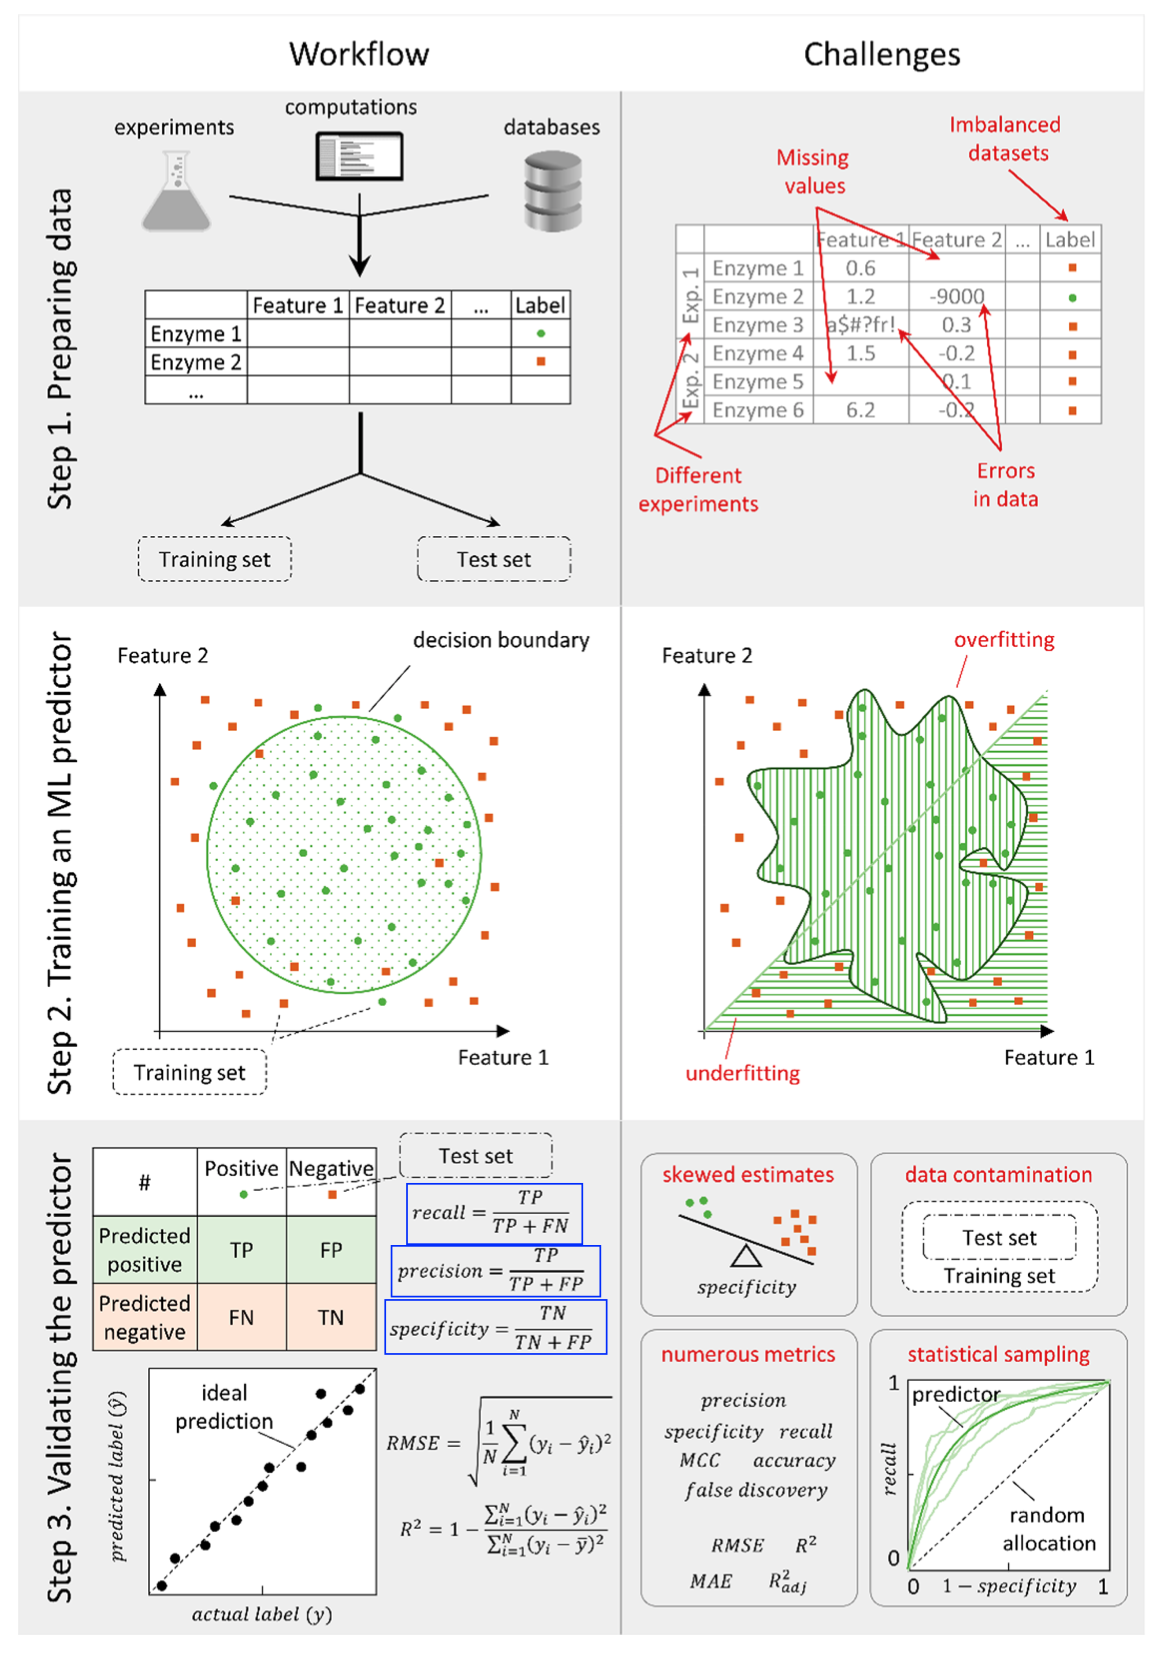
\includegraphics[scale=0.45]{Figura2.png}
\caption{Schematic workflow of constructing an ML predictor and associated challenges. }
\label{Figura2}
\end{figure}

Los principales tipos de Machine Learning son: Aprendizaje Supervisado y Aprendizaja No-Supervisado. En el aprensizaje no supervisado el objetivo es disminuir la alta dimensionalidad de los datos en uno de menor dimensión, o el de encontrar clústers en los datos.  En el aprendizaje supervisado varias propiedades objetivo tales como actividad o estabilidad de enzimas,  y el objetivo es diseñar un predictor que regrese etiquetas para datos no vistos considerando sus descriptores,  utilizando el conjunto de datos etiquetado como datos de entrenamiento.

\begin{Note}
Step 1: the data are usually turned into a table format and split into the training and test parts. Any errors, biases, or imbalances will be translated to the predictor’s performance and, hence, must be accounted for. Step 2: the predictor is trained on the training data set. For example, a decision boundary is derived that allows classifying future input based on whether data points are inside or outside the boundary. This is a balancing act between two extremes: explaining noise rather than fundamental dependencies (overfitting) or failure to account for complex dependencies in the data (underfitting). Step 3: the performance of the predictor is evaluated based on the test data set. For example, true and false positives and negatives and the associated measures are calculated or the root mean square error (RMSE) is calculated for continuous labels. The random nature of the initial data split as well as data imbalances might skew the evaluation, and numerous metrics used for evaluation vary in their robustness to different data skews. Even partial inclusion of the test set at any stage of ML predictor training is called data contamination and usually invalidates the final evaluation.

\end{Note}


La etapa que más tiempo consume es la de recolección de datos y su preparación para alimentar el algoritmo de ML, entonces los datos son introducidos en el subconjunto de entrenamiento, el resultado se utiliza para meujorar los parámetros del predictor de ML, mientras que el segundo se utiliza para la evaluación. 


\begin{Note}
\begin{itemize}

\item En problemas de clasificación con etiquetas binarias o etiquetas con una cantidad finita de opciones, la evaluación usualmente se realiza por medio de la matriz de confusión: el número de verdaderos/falsos positivos y negativos.

\begin{center}
\begin{tabular}{|c|c|c|}\hline
& Positivo & Negativo\\\hline
Predecido Positivo& TP & FP\\\hline
Predicido Negativo& FN & TN\\\hline
\end{tabular}
\end{center}

\item Para problemas de regresión con etiquetas de valores continuos usualmente se calcula la raíz del error cuadrático medio

\begin{equation}
RMSE=\sqrt{\frac{1}{N}\sum_{i=1}^{N}\left(y_{i}-\hat{y}\right)^2}
\end{equation}


\begin{equation}
R^2=1-\frac{\sum_{i=1}^{N}\left(y_{i}-\hat{y}\right)^2}{\sum_{i=1}^{N}\left(y_{i}-\overline{y}\right)^2}
\end{equation}

\end{itemize}

En cualquiera de los dos casos la evaluación final se lleva a cabo en el conjunto de prueba, el cuál es esencial dado que el último objetivo es obtener el predictor más general en los datos no utilizados para entrenar el algoritmo.
\end{Note}


\begin{Note}
Las siguientes métricas se utilizan para medir el rendimiento de un modelo en función de su capacidad para predecir correctamente las clases de un conjunto de datos. 

\begin{itemize}

\item \textbf{Recall (Recall o Sensibilidad):} Conocido como sensibilidad o tasa positiva real, mide la capacidad de un modelo para identificar correctamente todos los ejemplos positivos en un conjunto de datos. Se calcula como el número de verdaderos positivos dividido por la suma de verdaderos positivos y falsos negativos:

\begin{equation}
Recall = \frac{Verdaderos\ Positivos}{Verdaderos\ Positivos + Falsos\ Negativos}
\end{equation}

Un recall alto significa que el modelo es bueno para detectar los casos positivos, minimizando los falsos negativos. Es importante en situaciones donde los falsos negativos son costosos o críticos.


\item Precision (Precisión): La precisión mide la capacidad de un modelo para predecir correctamente los casos positivos entre todas las predicciones positivas que realiza. Se calcula como el número de verdaderos positivos dividido por la suma de verdaderos positivos y falsos positivos:

\begin{equation}
Precision = \frac{Verdaderos\ Positivos}{Verdaderos\ Positivos + Falsos\ Positivos}
\end{equation}

Una alta precisión significa que el modelo tiene una baja tasa de falsos positivos, es decir, que cuando predice una clase como positiva, es probable que sea correcta. La precisión es importante en situaciones en las que los falsos positivos son costosos o no deseados.

\item Specificity (Especificidad): La especificidad mide la capacidad de un modelo para predecir correctamente los casos negativos entre todas las predicciones negativas que realiza. También se conoce como tasa negativa real. Se calcula como el número de verdaderos negativos dividido por la suma de verdaderos negativos y falsos positivos:

\begin{equation}
Specificity=\frac{Verdaderos\ Negativos}{Verdaderos\ Negativos+Falsos\ Positivos}\end{equation}
Una alta especificidad indica que el modelo es bueno para identificar correctamente los casos negativos, minimizando los falsos positivos. Esto es importante en situaciones en las que los falsos positivos son costosos o problem\'aticos.
\end{itemize}
Estas métricas proporcionan una forma más completa de evaluar el rendimiento de un modelo de clasificación que simplemente mirar la precisión general. 
\end{Note}


En la ingeniería de proteínas, las similitudes en secuencias en ambos subconjuntos de datos deben ser tenidas en cuenta. Si alguna familia de proteínas está sobre representada en el conjunto de prueba, el predictor resultante puede resultar sesgado hacia la identificación de patrones válidos solamente para esta familia. Si algunas secuencias en el conjunto de prueba son muy cercanas al conjunto de entrenamiento, la evaluación final de desempeño dara resultados sobre optimistas. 

En el paso 2 de entrenamiento, es posible ajustar el predictor o seleccionar de entre varios predictores, usualmente por medio de validación $k-fold$. En este caso los datos de entrenamiento se subdividen en $K$ subconjuntos y el flujo de trabajo se repite $K$ veces, con cada uno de ellos utilizaods para la evaluación de los $K-1$ subconjuntos utilizados para entrenar. El reto principal en el paso 2 para cualquiern entrenamiento tipo ML supervisado es evitar el subajuste de los datos (sesgo alto) y el sobre ajuste (varianza grande). 

La \textbf{subestimación} ocurre cuando un predictor falla en encontrar patrones incluso en los datos de entrenamiento (cuando un modelo lineal simple se utiliza para explicar dependencia dependencias no lineales en los datos). El \textbf{sobreajuste} ocurre cuando el desempeño de un predictor disminuye notablemente en los datos de prueba en comparación con los datos de prueba, debido al aprendizaje de demasiado detalle y ruido, en lugar de identificar patrones generales. Tanto el subajuste como el sobreajuste pueden ser debido a la insuficiente calidad de los datos: ruido excesivo, características faltantes o irrelevantes, sesgo en los datos, o datos dispersos. También pueden ocurrir como consecuencia de una pobre aplicación del algoritmo: excesiva o insuficiente flexibilidad en la selección de los parámetros, protocolo de entrenamiento inapropiado, o contaminación de los datos de entrenamiento con el conjunto de datos de prueba.


\subsection{Bases de datos relevantes a Ingeniería de Enzima}


\subsubsection{The State of the Art in Data Accumulation}

Debido a que los algoritmos de ML se basan en los datos, la importancia de la calidad de los mismos utilizados para entrenamiento no puede ser subestimada.

Ejemplos de conjuntos de bases de datos, utilizadas en la ingeniería de enzimas, son secuencias de proteínas y estructuras de proteínas. La estabilidad y solubilidad de las proteínas son dos cualidades que han sido medidas por varias décadas y hasta la fecha. Tareas más desafiante es la anotar las propiedades catalíticas de las enzimas debido a la abundancia de tipos de reacciones, mecanismos, cofactores, amplios rangos de especificidades de sustratos, enancionselectividades y promiscuidades.


Las enzimas son catalizadores biológicos que facilitan una amplia variedad de reacciones químicas en los organismos vivos. Algunas razones por las cuales la anotación de sus propiedades catalíticas es complicada son:

\begin{itemize}
\item \textbf{Tipos de reacciones diversos:} Las enzimas pueden catalizar una amplia gama de reacciones químicas, incluyendo reacciones de oxidación-reducción, hidrólisis, condensación, isomerización y más. Cada tipo de reacción involucra mecanismos químicos y sustratos diferentes.

\item \textbf{Mecanismos:} Incluso dentro de un solo tipo de reacción, las enzimas pueden emplear múltiples mecanismos. Comprender el mecanismo específico utilizado por una enzima requiere un conocimiento detallado de la estructura de la enzima y de su sitio activo.

\item \textbf{Cofactores:} Muchas enzimas requieren cofactores, como iones metálicos o coenzimas, para catalizar reacciones de manera efectiva. Identificar los cofactores necesarios para cada enzima es esencial para la anotación.

\item \textbf{Condiciones de reacción:} La actividad enzimática puede depender en gran medida de las condiciones ambientales, incluyendo la temperatura, el pH y la fuerza iónica. La anotación de las condiciones óptimas para la actividad enzimática es crucial.

\item \textbf{Especificidades de sustratos:} Las enzimas pueden ser altamente específicas para ciertos sustratos, reconociéndolos con alta afinidad, mientras que otras son más promiscuas y pueden unirse a una variedad de sustratos. La caracterización de la especificidad de sustratos es compleja.

\item \textbf{Enantioselectividades:} Algunas enzimas pueden discriminar entre enantiómeros (isómeros de imagen especular) de una molécula, catalizando reacciones con alta selectividad por un enantiómero. La anotación de esta propiedad implica comprender la estereoquímica.

\item \textbf{Promiscuidades:} Las enzimas pueden exhibir actividades promiscuas, catalizando reacciones diferentes a su función principal. Detectar y caracterizar tales promiscuidades es complicado.
\end{itemize}

\subsubsection{Current Challenges Related to Databases}

Si la dependencia que se busca no se encuentra en los datos disponibles, no importa la cantidad de nuevos datos ayudarán a mejorar la calidad del predictor de ML. En el caso de la ingeniería de enzimas se espera que las funciones enzimáticas estén codificadas en las secuencias y así depender en las propiedades físico-químicas de los aminoácidos, de aquí que la cantidad y la calidad de los datos en las bases de datos sean de importancia para diseñar un predictor de ML.


La falta de estándares en los reportes resulta en pérdida de información o valores erróneos para algunos descriptores. A esto hay que agregar la falta de protocolos robustos en los análisis de datos, como por ejemplo aquellos utilizados para ajuste de curvas para determinar las temperaturas de fusión o constantes cinéticas. Otro factor es que los recientes avances vuelven obsoletos resultados previos. La curación manual ayuda mejorar la calidad de los datos, sin embargo no se encuentra excenta de errores de anotación de las funciones de las proteínas y errores de propagación a partir de resultados previamente refutados.

Este tipo de procedimientos, verificación manual, puede incluir la limpieza o formato de datos para que sean amigables con ML. Uno de los principios más populares es \textbf{FAIR}, por sus siglas en inglés, Findable, Accesible, Interoperables y Reutilizables, debería de facilitar a las computadoras para que de manera automática pueda encontrar y utilizar los datos. Para las enzimas la guía estándar para reportar datos de enzimas (STRENDA) debería de aumentar la calidad de los datos, especialmente en bases de datos (bdd) heterogéneas recopiladas de diversas fuentes.


El desarrollo de nuevos predictores de ML ha incrementado considerablemente la demanda de mejora de las bdd existentes, así como la generación de nuevas bdd uniformes y representativas de mayor calidad. 

Existen varias nuevas técnicas emergentes tales como

\begin{itemize}
\item[i ] Secuenciación de nueva generación.
\item[ii ] Clasificación de células activadas por fluorescencia.
\item[iii ]  Exploración mutacional profunda, y  
\item[iv ] Microfluidos

\end{itemize}

\subsubsection{Emerging Methods for High-Throughput Data
Collection}

Avances tecnológicos hacia la miniaturización, automatización y paralelización han generado tecnologías eficientes de nuevos métodos de investigación experimental con capacidades incomparables. Secuenciación de nueva generación (NGS) ha revolucionado la investigación genómica, habilitado el acceso a datos moleculares fundamentales y revelado firmas genómicas  y transcriptomicas \cite{47,48}.

La capacidad de secuencias en el rango de gigabases por ejecución del instrumento permite secuencias el genoma humano en su totalidad en tan sólo un día. 

Múltiples instrumentos comerciales de segunda generación disponibles ofrecen mayor capacidad y precisión. Métodos de tercera generación recientemente introducidos (lectura larga)  que emplean secuenciación en tiempo real de moléculas \cite{50} o secuenciación de nanoporos \cite{51} resuelve las limitaciones de lecturas cortas, como el sesgo de GC o mapear elementos repetitivos

Mientas el avance de la tecnología de secuenciación proporciona una gran cantidad de secuencias de datos, para la mayoría de estas entradas, las anotaciones estructurales y anotaciones funcionales aún están perdidas. 


Como siguiente paso, se está centrando en el desarrollo de nuevos métodos experimentales efectivos para recopilar información funcional y estructural. 

La clasificación de células activadas por fluorescencia (FACS) es una tecnología ampliamente disponible que permite el cribado de hasta 108 variantes de enzimas por día. La FACS requiere que los sustratos fluorogénicos estén atrapados dentro o en la superficie de la célula para vincular el genotipo y el fenotipo. Alternativamente, se utiliza la clasificación de enzimas encapsuladas junto con su ADN codificador y un sustrato fluorogénico en perlas de hidrogel.

Cuando se combinan con la secuenciación de próxima generación, los ensayos de alto rendimiento representan una estrategia poderosa para analizar de manera integral las relaciones entre secuencia y función en las enzimas \cite{52,55}. Este enfoque, llamado escaneo mutacional profundo (DMS por sus siglas en inglés), vincula el genotipo con el fenotipo sin necesidad de procesos laboriosos que involucren la purificación y caracterización de proteínas. Durante el proceso, se sintetiza una gran biblioteca de secuencias mutantes, seguida de la selección de fenotipos expresados. Luego, la secuenciación de la biblioteca antes y después de la selección cuantifica la aptitud de cada mutante. De esta manera, el DMS proporciona un método rápido y sencillo para inferir los determinantes de la secuencia de la estabilidad y la función de las proteínas\cite{52,56,57}. El DMS se ha utilizado como una estrategia experimental alternativa para la determinación de la estructura de las proteínas.


\subsection{MACHINE LEARNING APPLICATIONS TO ENZYME ENGINEERING}

\begin{itemize}

\item Despite being a relatively new field of study,  machine Learning for enzyme engineering has already been applied for several challenging predictions.  First consider predictors aimed at elucidating the structure function relationships crucial for enzymes on both sides:

\begin{itemize}
\item predicting the structure for a known sequence, and 

\item predicting the catalytic activity or substrate specificity for a known sequence-structure. 
\item solubility and stability, from the point of view of amino acid substitutions,

\end{itemize}

\item The protein structure prediction is one of the longest-standing challenges in biochemistry, as the number of resolved structures is dramatically lagging behind the number of known sequences.

\item Over 145000 structures have been released in the Protein Data Bank, but this is still nowhere near over 215 million publicly available protein sequences\cite{28}. 

\item Nevertheless, even despite a relatively small data set size in comparison to millions of data points usually available for this method, deep neural networks showed most the notable results in the latest biennial assessment of protein structure prediction methods, CASP13. 

\begin{Note}
The AlphaFold network was trained on the PDB entries to predict the distances between C-beta atoms of residues using multiple sequence alignments\cite{60} and received the highest score at the competition. Out of 124 targets, around two-thirds of AlphaFold predictions had a $GDT_TS$ score above 50, which is indicative of a topologically correct structure \cite{61}.
\end{Note}

\item Apart from predicting protein structures, predicting catalytic activities is another active field of research currently. 

\item Computational methods for the protein function prediction range from sequence-to structure-based and from gene-to genome- and interactome-based\cite{62}. 


\item Several initiatives similar to the CASP competition have already been proposed to address the functional annotation of enzymes, namely Enzyme Function Initiative (EFI), the Computational Bridges to Experiments initiative (COMBREX), and the Critical Assessment of Function Annotation community-driven experiment (CAFA). 


\item Successful attempts to apply ML to assign enzyme EC numbers using predicted 3D structures \cite{63} or exploiting sequence similarities \cite{64} have already been made. 

\item Recently, deep learning was also applied to predict EC numbers on the basis of a protein sequence using both sequence-length-dependent features, such as raw sequence one-hot encoding, and sequence-length-independent features, such as functional domain encoding \cite{65}.


\item The former type of features introduced non uniformity in feature dimensionality, and the authors presented a framework to perform simultaneously dimensionality uniformization,  feature selection, and  classification model training. 

\item The large data sets of enzyme structures and activities accumulated to date already allow using deep learning in the engineering of catalytic activity. 


\item A more precise functional prediction is possible by restricting ML training to a particular family of enzymes, which comes at the cost of much smaller data sets available for training. This problem may be tackled by applying high-throughput data collection methods mentioned before. The authors of the recently released GT-predict \cite{66} selected for their analysis the glycosyltransferase superfamily 1, a group of enzymes with highly diverse substrates. 


\begin{Note}
Data from the label-free mass spectroscopy-based assay of 91 substrates and 54 enzymes derived from the plant Arabidopsis thaliana were used for functional prediction. The authors trained sequence-based decision trees, systematically varying combinations of physicochemical  properties,  e.g. log P, molecular area, and number/type of nuclephilic groups, and structural information, e.g.  scaffold type and functional groups. The resulting predictor was successfully tested on four individually selected gene sequences as well as two complete families of enzymes from four different organisms, which highlights the tremendous potential of training ML predictors on the newly acquired data from high-throughput data collection methods. 
\end{Note}

\item In their recent paper \cite{35} Han and coauthors considered seven different binary and continuous ML algorithms: logistic regression, decision tree, support vector machines,  Naive Bayes,  conditional random forest,  XGBoost, and artificial neural networks. 

\item The authors attempted to use generative adversarial networks to synthesize more data. This is a pair of two neural networks competing against each other: one learns to generate artifficial examples and the other to distinguish them from real data. 

\item Another point of view on protein solubility prediction is studying the effects of individual mutations. The recent successes in the application of deep mutational scanning to collect the data on protein solubility changes upon mutations\cite{68} are likely to promote the development of more sophisticated ML-based protein solubility predictors in the nearest future. 

\item Predicting the effects of amino acid substitutions is not only limited to solubility: stability, substrate specificity, catalytic activity, and enantioselectivity can also be targeted if sufficient data are available.


\item Protein stability predictors are perhaps those with the most abundant data sets of this type available for ML training

\item The authors also presented a random forest classiffier trained using 1106 features from the following groups: experimental conditions, conservation and coevolution scores for mutated positions, amino acid substitutions and their physicochemical properties, neighborhood features for 11 positions before and after substitution sites, and thermodynamic sequence-based features extracted from ProtDCal \cite{69}. 


\item PON-tstab is a three-class predictor (stability increasing, decreasing, unchanged) and achieved the correct prediction ratio of around 0.5 versus the value 0.33 for a random predictor. This implies that, even with a data set of higher quality, predicting protein stability remains an extremely challenging task \cite{5}.

\item Another intriguing application of ML in protein engineering is to design smart combinatorial libraries for directed protein evolution\cite{70}. This has the potential to both reduce the experimental effort and improve the exploration of the sequence space by mutating multiple positions simultaneously. Moreover, it can approximate the empirical fitness landscape to suggest a refined set of variants for the next round of screening.

\item Wu et al\cite{71} used ML assisted directed evolution to engineer an enzyme for a new stereodivergent carbon-silicon bond formation. The authors selected the reaction of phenyldimethyl silane with ethyl 2-diazopropanoate catalyzed by a putative nitric oxide dioxygenase from Rhodothermus marinus. They tested a variety of ML algorithms such as linear and kernel models, shallow neural networks, and ensemble methods to improve the enzyme enantioselectivity.

\end{itemize}


 
\subsubsection{Current Challenges Related to ML-Aided}

\begin{itemize}

\item One of the main challenges in applications of ML to enzyme engineering stems from the intrinsic multidisciplinarity of the approach. Biochemists, molecular biologists, mathematicians, and computer scientists have to find a common language to clarify goals, carry out rigorous analysis and training, and avoid common pitfalls, wrongful usage of methods, and misinterpretations.

\item The No Free Lunch theorem \cite{85} claims that no single ML method is superior to others a priori \cite{86}; 


\item A thorough understanding of the data types to be used and problems to be solved is essential in the development of efficient predictors. The current shift toward new and more complex ML methods, namely aggregating several algorithms into hybrid meta-predictors, hyperparameter optimization with many training subcycles, feature learning, and the fusion of ML-based and classical bioinformatics tools in a single predictor, will further challenge the crosstalk between disciplines necessary for the development of efficient and robust predictors in enzyme engineering.

\item With the continuous growth of ML applications in enzyme engineering, the need for robust comparison of various predictors is of growing importance. This comparison is mainly obstructed by the lack of both standardized protocols for comparison and new data sets for testing. 

\item The lack of benchmark data sets, discrepancies in the performance measurements used, inaccurate or insufficient disclosure in publications, and the difficulty in finding reviewers with sufficiently broad expertise \cite{87} are among the most pressing issues. 

\item Researchers working on some applications with a long track record in bioinformatics, such as protein structure or function predictions, have already established several platforms that can be used for comparison of the ML predictors, i.e. CASP, CAFA, EFI, and COMBREX.

\item Other applications have yet to see similar initiatives as at least three key ingredients are necessary: 

\begin{itemize}
\item[i] a sufficiently large community of researchers working on development of such applications, 
\item[ii] a sufficient amount of new high-quality data being collected regularly, and 
\item[iii] a leader that will take on responsibility and invest time and effort into coordinating this activity. 
\end{itemize}

\item Few papers go beyond simple ROC analysis: e.g., resample cross-validation to estimate its statistical significance, explore the reasons for weak predictions, and analyze learning curves. Why does a particular predictor have a better performance? What features are critical for the performance of a predictor on a global scale? What ranges for feature values and what parts of the feature space are most critical for a particular data point to be classiffied correctly?
\end{itemize}

\subsection{Emerging Trends in ML-Based Methods for Enzyme Engineering}


\begin{itemize}
\item With the accumulation of more data by virtue of the emerging high-throughput experimental methods, the development of benchmark data sets and unified performance measurements is only a matter of time.

\item Recently, an intriguing algorithm based on semisupervised learning has been presented to allow benchmarking in five different prediction tasks related to protein engineering, including secondary structure, fluorescence landscape, and stability landscape predictions \cite{88}

\item As the data generation is streamlined, a data set from a single experiment is starting to have the size large enough for training ML algorithms to guide the design of future experiments, as was the case in the development of stereodivergent carbon silicon bond formation\cite{71} and the application of Gaussian processes to the directed evolution of cytochromes\cite{89}.

\item The increase in the available data will prompt more extensive use of deep neural networks. Sophisticated neural network architectures, such as recurrent or graph-based neural networks, simultaneous training of several types of predictors (multitasking), combining structurally different input data (multimodal design), ML-based modeling of data sets (generative models), and retraining predictors used in one area by new data from another area (transfer learning) have only recently been applied in genomics\cite{14}


\item Several attempts have recently been made to apply some of those advanced techniques to proteins: using generative models to create soluble and functional malate dehydrogenase variants\cite{90} or predict mutational effects with high correlation with those actually observed in 42 high-throughput deep mutational scanning experiments\cite{91}


\item More data will also allow improving the existing methods, i.e. learning the optimal architecture of a predictor from the data (hyperparameter optimization)\cite{92}, smart aggregation of several predictions from multiple methods\cite{93}, and introducing robust conffidence scores for predictions\cite{94}. In enzyme engineering, this new level of algorithmic complexity will further save time and resources wasted on validating misleading predictions but will also require more sophisticated computer architecture, e.g. an increased use of parallel computing and stochastic training methods, which have already become standard techniques for the acceleration of deep neural network training.



\item Another noticeable trend in ML is toward interpretable and explainable predictors\cite{95}. Apart from the global importance of features for ML predictors, feature importance scores calculated for each input example\cite{96,97} may help explain why a particular prediction was made for each input data point. 


\item Interpretable algorithms can aid in smart biocatalyst design. For instance, instead of simply screening all the possible mutations with an ML-based tool to improve a target property, researchers can make use of designing variants on the basis of the structure of a predictor using adaptive sampling\cite{98}. 



\item Such an approach favors predictors whose parameters can provide such guidance: e.g., linear predictors over more flexible yet harder to interpret artifficial neural networks (Figure 3). Linear predictors allow analytical design on the basis of the coefficients \cite{99} in contrast, sophisticated predictors are usually prone to pathological behavior, i.e. sudden misclassiffication after a slight and almost imperceptible perturbation of input\cite{100}.


\item Another promising approach is to use interpretable architectures of predictors already at the design stage, e.g. the visible neural networks\cite{101}. The design of such networks is guided by the knowledge of the underlying biological mechanism, e.g. the choice of layers and the connections between layers may mimic the hierarchical organization of transcriptional regulatory factors in the cell nucleus.


\end{itemize}










\section{Artículo 2: A general model to predict small molecule substrates of enzymes based on machine and deep learning}

\subsection{About the existence techniques}

\begin{Note}
\begin{itemize}
\item Las enzimas han evolucionado de manera eficiente para catalizar eficientemente una o más reacciones químicas incrementando las tasas de reacción hasta más de un millón. Además la mayoría de las enzimas son promiscuas, es decir, se catalizan más, fisiológicamente irrelevantes o reacciones inofensivas \cite{2.2, 2.4}

\item Un mapeo exhaustivo de las relaciones enzima-sustrato desempeña un papel crucial en la investigación farmacéutica y bioingeniería, por ejemplo, para la producción de medicamentos, productos químicos, alimentos y biocombustibles \cite{2.5, 2.6,2.7}.


\item La base de datos UniProt contiene entradas de más de 36 millones de enzimas diferentes, más del $99\%$ de ellas carecen de anotaciones de alta calidad de las reacciones catalizadas. Se están realizando esfuerzos para desarrollar métodos de alto rendicmiento para la determinación experimentarl de relaciones entre enzimas y sustratos, esfuerzos que se encuentran en su etapa inicial\cite{2.9,2.10,2.11}.


\item Se han realizado esfuerzos por desarrollar metodos de alto rendimiento para determinar las relaciones experimentales de las relaciones enzima-sustratos. El objetivo en este trabajo es desarrollar un modelo de Machine Learning (ML) con la capacidad de predecir las relaciones enzima-sustratos a traves de todas las proteínas, por tanto contar con una herramienta que ayude a focalizar esfuerzos experimentales en pares de moléculas de pequeñas enzimas parece ser biológicamente relevantes. 

\item Los principales retos son que la representación numérica de caeda enzima que máximamente informativa para la predicción rio abajo, para ser lo más ampliamente posible, estas representaciones deben basarse de manera única en la secuencia primaria de las enzimas sin información adicional. Otro reto es que las bases de datos públicas de enzimas, solamente enlista instancias positivas, es decir, moleculas con las cuales las enzimas despliegan actividades medibes \cite{2.13}. 

\end{itemize}
\end{Note}

\subsection{About the ML techniques}

\begin{Note}
\begin{itemize}
\item Para entrenar un modelo de predicción, es necesario idear una estrategia automatizada para obtener instancias adecuadas de enzimas y pequeñas moléculas que sean negativas y no se unan. Los enfoques de aprendizaje automático existentes para predecir pares enzima-sustrato fueron desarrollados específicamente para familias de enzimas pequeñas para las cuales existen conjuntos de datos de entrenamiento inusualmente completos \cite{2.13}-\cite{2.18}.

\item Mou et al.\cite{2.14} desarrollaron modelos para predecir los sustratos de las nitrilasas bacterianas, utilizando características de entrada basadas en las estructuras tridimensionales y sitios activos de las enzimas. Entrenaron varios modelos de aprendizaje automático basados en evidencia experimental para todas las posibles combinaciones de enzima y molécula pequeña dentro del alcance de predicción de los modelos (N = 240). 


\item Yang et al.\cite{2.15} predijeron el alcance de sustratos de las glicosiltransferasas de plantas entre un conjunto predefinido de moléculas pequeñas. Entrenaron un modelo basado en árboles de decisión con un conjunto de datos que cubría casi todas las posibles combinaciones de enzimas y moléculas pequeñas relevantes. 


\item Pertusi et al.\cite{2.13} entrenaron cuatro máquinas de vectores de soporte (SVM) diferentes, cada una para una enzima específica. Como características de entrada, sus modelos solo utilizan información sobre los sustratos (potenciales), así como no sustratos extraídos manualmente de la literatura; no se utilizó información explícita sobre las enzimas.


\item Roettig et al.\cite{2.16} y Chevrette et al.\cite{2.17} predijeron los alcances de sustratos de familias de enzimas pequeñas, entrenando modelos de aprendizaje automático con información estructural relacionada con los sitios activos de las enzimas. 


\item Visani et al.\cite{2.19} implementaron un modelo de aprendizaje automático general para predecir clases EC adecuadas para un sustrato dado. Para entrenar este modelo, se utilizaron todas las clases EC que no están asociadas con un sustrato específico como puntos de datos negativos, lo que resultó en una baja proporción promedio de positivos a negativos de 0.0032. Visani et al. no utilizaron información sobre las enzimas más allá de la clase EC como entrada del modelo, y por lo tanto, el modelo no puede distinguir entre diferentes enzimas asignadas a la misma clase EC.


\end{itemize}
\end{Note}

\subsection{About the approuch of existing models}

\begin{Note}

\begin{itemize}
\item Todos estos modelos no pueden aplicarse a enzimas individuales o intentan predecir sustratos solo para una enzima o familia de enzimas. 

\item Aquellos modelos que hacen predicciones para enzimas específicas se basan en datos de entrenamiento experimentales muy densos, es decir, resultados experimentales para todas o casi todas las posibles combinaciones de enzima-sustrato.

\item Para la gran mayoría de familias de enzimas, no está disponible un conjunto de datos de entrenamiento tan extenso. 

\item Hasta el momento, no ha habido intentos publicados de formular y entrenar un modelo general que pueda aplicarse para predecir sustratos para enzimas específicas en familias de enzimas ampliamente diferentes. 

\item Los modelos de aprendizaje profundo se han utilizado para predecir funciones de enzimas ya sea prediciendo su asignación a clases EC20–22, o prediciendo dominios funcionales dentro de la secuencia de proteínas\cite{2.23}

\item Predecir directamente sustratos específicos para enzimas representa un paso importante más allá de esos métodos previos y puede ayudar a predecir la función de la enzima de manera más específica y precisa.

\item Los enfoques de vanguardia en este dominio son basados en características, es decir, se utilizan representaciones numéricas de la proteína y la molécula del sustrato como entrada para modelos de aprendizaje automático\cite{2.25}-\cite{2.29}. 

\item Como descripciones numéricas de la molécula del sustrato, estos enfoques utilizan representaciones SMILES30, huellas digitales expertas\cite{2.31} o huellas digitales creadas con redes neuronales gráficas\cite{2.32,2.33}. 

\item Las proteínas suelen codificarse numéricamente mediante representaciones basadas en el aprendizaje profundo de las secuencias de aminoácidos\cite{2.34}-\cite{2.36}.

\end{itemize}

\end{Note}

\subsection{About the work in this article}

\begin{Note}
\begin{itemize}

\item In this work, we go beyond the current state-of-the-art by creating maximally informative protein representations, using a customized,  task-specific version of the ESM-1b transformer model \cite{2.34}. 

\item The model contains an extra 1280-dimensional token, which was trained end-to-end to store enzyme-related information salient to the downstream prediction task. 

\item This general approach was first introduced for natural language processing37, but has not yet been applied to protein feature prediction. 

\item We created negative training examples using data augmentation, by randomly sampling small molecules similar to the substrates in experimentally confirmed enzyme-substrate pairs.

\item we sampled all negative data points from a limited set of metabolites, the set of ~ 1400 substrates that occur among all experimentally confirmed enzyme-substrate pairs of our dataset. 

\item Thus, we do not sample from the space of all possible alternative reactants similar to the true substrates, but only consider small molecules likely to occur in at least some biological cells. 

\item While many enzymes are rather promiscuous 2-4, it is likely that most of the potential secondary substrates are not contained in this restricted set for any given enzyme, and hence the chance of sampling false negative data points was likely small. 

\item We numerically represented all small molecules with task-specific fingerprints that we created with graph neural networks (GNNs)\cite{2.38,2.39,2.40}. 

\item A gradient-boosted decision tree model was trained on the combined protein and small molecule representations for a high-quality dataset with ~18,000 very diverse, experimentally confirmed positive enzyme-substrate pairs. 

\item The resulting Enzyme Substrate Prediction model-ESP-achieves high prediction accuracy for those ~1400 substrates that have been part of our training set and outperforms previously published enzyme family-specific prediction models.
\end{itemize}

\end{Note}

\subsection{About the obtained results}

\begin{Note}
\begin{itemize}


\item A data set with experimentally confirmed enzyme-substrate pairs using the GO annotation database  for Uniprot IDs\cite{2.41} was created.

\item For training the machine learning models, they extracted 18,351 enzyme-substrate pairs with experimental evidence for binding, comprised of 12,156 unique enzymes and 1379 unique metabolites. 

\item Also extracted 274,030 enzyme-substrate pairs with phylogenetically inferred evidence, i.e., these enzymes are evolutionarily closely related to enzymes associated with the same reactions. These guilt by associations assignments are much less reliable than direct experimental evidence, and we only used them during pre-training to create task-specific enzyme representations-numerical vectors aimed at capturing information relevant to the prediction task from the enzyme amino acid sequences. 

\item The validations demonstrate that using phylogenetically inferred functions for the construction of appropriate enzyme representations has a positive effect on the prediction of experimentally confirmed enzyme-substrate pairs.

\item There is no systematic information on negative enzyme-small molecule pairs, i.e., pairs where the molecule is not a substrate of the enzyme.

\item It was hypothesized that such negative data points could be created  artificially through random sampling, which is a common strategy in  classification tasks that lack negative training data \cite{2.42}.


\item Only were considered small molecules included among the experimentally confirmed enzyme-substrate pairs in our dataset. 

\item Among such a limited and biased subset, enzymes are quite specific catalyst, and therefore most of the potential secondary substrates are not included for the majority of enzymes.

\item It was assumed that the frequency of incorrectly created negative labels is sufficiently low o not adversely affect model performance. This assumption was confirmed by the high model accuracy on independent test data.

\item To select putatively non-binding small molecules that are structurally similar to the known substrates, it was used a similarity score based on molecular fingerprints with values ranging from 0 (no similarity) to 1 (identity; see Methods, sampling negative data points). 

\item For every positive enzyme-substrate pair, it was sampled three molecules with similarity scores between 0.75 and 0.95 to the actual substrate of the enzyme, and used them to construct negative enzyme-molecule pairs. 

\item it was opted for creating more negative data points than positive data points, as this not only provided us with more data, but it also more closely reflects the true distribution of positive and negative data points compared to a balanced distribution.

\item Our final dataset comprises 69,365 entries. We split this data into a training set ($80\%$) and a test set ($20\%$). 

\item In many machine learning domains, it is standard practice to split the data into training and test set completely at random. However, when dealing with protein sequences, this strategy often leads to test sets with amino acid sequences that are almost identical to those of proteins in the training set. 

\item It is common practice to split such datasets into training, validation, and test sets based on protein sequences similarities \cite{2.44}.

\item It was made sure that no enzyme in the test set has a sequence identity higher than $80\%$ compared to any enzyme in the training set.  To show that despite this sequence-based partitioning, enzymes from the training and test sets follow the same distribution, we used dimensionality reduction to map all enzymes to a two-dimensional subspace and plotted the corresponding data points. 

\item To evaluate how well the final  model performs for different levels of enzyme similarities, it was  divided the test set further into three subsets with maximal sequence identities between $0–40\%$, $40–60\%$, and $60–80\%$ compared to all enzymes in the training set.

\item For the numerical encoding, one classiffies  bond types and calculates feature vectors with information about every atom (types, masses, valences, atomic numbers, atom charges, and number of attached hydrogen atoms)\cite{2.31}.  Afterwards, these identifiers are updated for a fixed number of steps by iteratively applying predefined functions to summarize aspects of neighboring atoms and bonds. 

\item After the iteration process, all identiffiers are converted into a single binary vector with structural information about the molecule. \textsl{The number of iterations and the dimension of the fingerprint can be chosen freely, in this case they were set to the default values of 3 and 1024, respectively, also was created 512- and 2048-dimensional ECFPs, but these led to slightly inferior predictions. Using ECFPs can lead to identical representations for structurally very similar molecules, e.g., for some molecules that differ only by the length of a chain of carbon atoms.  In our dataset, 182 out of 1379 different molecules shared an identical fingerprint with a structurally similar molecule.}

\item As an alternative to expert-crafted fingerprints such as ECFPs, neural networks can be used to learn how to map graph representations of small molecules to numerical vectors, such networks are referred to as graph neural networks (GNNs)\cite{2.38,2.39,2.40} 

\item We trained a GNN for the binary task of predicting if a small molecule is a substrate for a given enzyme. While training for this task, the GNN is challenged to store all information about the small molecule that is relevant for solving the prediction task in a single numerical vector. 

\item After training, were extracted these 100-dimensional task-specific vectors for all small molecules in our dataset. It has been observed that pre-training GNNs for a related task can signifficantly improve model performance\cite{2.45,2.46}.

\item Thus,  first were pre-trained the GNN for the related task of predicting the Michaelis constants $K$M of enzyme-substrate pairs (see Methods,  pre-training indeed improved prediction performance significantly.  In contrast to ECFPs, GNN-generated fingerprints lead to much fewer cases of identical representations for different molecules. 

\item In the dataset, identical fingerprints occurred for 42 out of 1379 molecules training of $ESM-1b, ~15\%$ of the amino acids in a protein’s sequence are randomly masked and the model is trained to predict the identity of the masked amino acids. This training procedure forces the model to store both local and global information about the protein sequence in one 1280-dimensional representation vector for each individual amino acid. 

\item In order to create a single fixed-length numerical representation of the whole protein, one typically calculates the element-wise mean across all amino acid representations\cite{2.34,2.35,2.49}. it was refered to these protein representations as ESM-1b vectors

\begin{Note}
Simply taking the element-wise mean results in information loss and does not consider the task for which the representations shall be used, which can lead to subpar performance. To overcome these issues, we created task-specific enzyme representations optimized for the prediction of enzyme-substrate pairs. 

We slightly modified  the architecture of the ESM-1b model, adding one additional 1280-dimensional token to represent the complete enzyme, intended to capture information salient to the downstream prediction task. The extra token is not adding input information to the model, but it allows an easier extraction of enzyme information from the trained model. This whole-enzyme representation was updated in the same way as the regular ESM-1b amino acid representations.
\end{Note}

\item After a predefined number of update steps, the enzyme representation was concatenated with the small molecule ECFP-vector. The combined vector was used as the input for a fully connected neural network (FCNN), which was then trained end-to-end to predict whether the small molecule is a substrate for the enzyme. 

\item This approach facilitates the construction of a single, optimized, task-specific representation. The ESM-1b model contains many parameters and thus requires substantial training data. Therefore, in the pre-training that produces the task-specific enzyme representations, we added phylogenetically inferred evidence to our training set; this resulted in a total of ~287,000 data points used for training the task-specific enzyme representation. 


\item After training, we used the network to extract the 1280-dimensional task-specific representations for all enzymes in our
dataset, these representations are called ESM-1bts vectors.

\item The ESM-1b model is a state-of-the-art transformer network\cite{2.47}, trained with ~27 million proteins from the UniRef dataset\cite{2.48} in a self-supervised fashion\cite{2.34}. This model takes an amino acid sequence as its input and puts out a numerical representation of the sequence; these representations are often referred to as protein embeddings.


\item we estimated prediction quality on our test set when using machine learning models with each of the four combinations of enzyme and small molecule representations. In each case, we concatenated one of the two 1280-dimensional enzyme representations with one of the two small molecule representations to create a single input vector for every enzyme- small molecule pair. 

\item We used these inputs to train gradient-boosted decision tree models\cite{2.50} for the binary classification task of predicting whether the small molecule is a substrate for the enzyme.

\item We performed hyperparameter optimizations for all four models, including the parameters learning rate, depth of trees, number of iterations, and regularization coefficients.

\item For this, we performed a random grid search with a 5-fold cross-validation (CV) on the training set. To challenge the model to learn to predict the substrate scope of enzymes not included in the training data, we made sure that each enzyme occurred in only one of the five subsets used for cross-validation. 
 
\item To account for the higher number of negative compared to positive training data, we also included a weight parameter that lowered the influence of the negative data points. 

\item After hyperparameter optimization, the models were trained with the best  set of hyperparameters on the whole training set and were validated on our independent test set, which had not been used for model training or hyperparameter selection. It is noteworthy that for some input combinations, the accuracies on the test set are higher than the accuracies achieved during cross-validation.

\item This improved performance on the test set may result from the fact that before validation on the test set, models are trained with approximately 11,000 more samples than before each cross-validation; the number of training samples has a substantial influence on model performance.

\item To compare the gradient boosting model to alternative machine learning models, we also trained a logistic regression model and a
random forest model for the task of predicting enzyme-substrate pairs from the combined ESM-1bts and GNN vectors. However, these models performed worse compared to the gradient boosting model. 

\item To investigate the importance of the added token for the observed superior performance, we alternatively re-trained the ESM-1b
without such an extra token.

\item Good predictions even for unseen enzymes It appears likely that prediction quality is best for enzymes that are highly similar to enzymes in the training set, and decreases for enzymes that are increasingly dissimilar to the enzymes used for training. 

\item How strong is that dependence? To answer this question, we first calculated the maximal enzyme sequence identity compared to
the enzymes in the training set for all 2291 enzymes in the test set. Next, we split the test set into three subgroups: data points with
enzymes with a maximal sequence identity to training data between 0 and $40\%$, between $40\%$ and $60\%$ and between $60\%$ and $80\%$.


\item It was shown model performance is highest for enzymes that are similar to proteins in the training set. Similarly, it appears likely that the model performs better when making predictions for small molecules that are also in the training set. To test this hypothesis, we divided the test set into data points with small molecules that occurred in the training set (N = 13,459) and those with small molecules that did not occur in the training set (N = 530).


\item The ESP model does not perform well for data points with small molecules not present in the training set. When considering only
enzyme-small molecules pairs with small molecules not represented in the training set and an enzyme sequence identity level of $0–40\%$ compared to the training data, ESP achieves an accuracy of $71\%$, ROC- AUC score 0.59, and MCC 0.15. At an enzyme sequence identity level of $40–60\%$, accuracy improves to $83\%$, with ROC-AUC score 0.78, and MCC 0.25 for unseen small molecules.


\item For those test data points with small molecules not present in the training set, we wondered if a high similarity of the small molecule compared to at least one substrate in the training set leads to improved predictions, analogous to what we observed for enzymes with higher sequence identities. 

\item For each small molecules not present in the training set, we calculated the maximal pairwise similarity score compared to all substrates in the training set. 

\item we conclude that ESP only achieves high accuracies for new enzyme-small molecule pairs if the small molecule was present among the ~1 400 substrates of our training set.


\item How many training data points with identical substrates are needed to achieve good model performance? For every small molecule in the test set, we counted how many times the same molecule occurs as an experimentally confirmed substrate in the training set. 

\item Model performance increases with increased training set size The previous subsections suggest that a bigger training set with a more diverse set of enzymes and small molecules should lead to improved performance. However, using more data does not guarantee an improved model performance. 

\item To test how our model performs with different amounts of training data and to analyze if more data is expected to lead to higher generalizability, we trained the gradient boosting model with different training set sizes, ranging from $30\%$ to $100\%$ of the available training data.

\item Internally, our trained classification  model does not simply output the positive or negative class as a prediction. Mou et al.\cite{2.14} trained four different machine learning models (logistic regression, random forest, gradient-boosted decision trees,
and support vector machines) to predict substrates of bacterial nitrilases. 

\item For model training and validation, they used a dataset with all possible combinations of 12 enzymes and 20 small molecules
(N = 240), randomly split into $80\%$ training data and $20\%$ test data. Instead, it outputs a prediction score between 0 and 1,Yang et al.15 published a decision tree-based model, GT-Predict, for predicting the substrate scope of glycosyltransferases of plants.All software was coded in Python57. We implemented and trained the neural networks using the deep learning library PyTorch58. We fitted the gradient boosting models using the library XGBoost50.
\end{itemize}

\end{Note}



\begin{Note}
Deep learning-based kcat prediction enables improved enzyme-constrained model reconstruction

\begin{itemize}


\item Deep learning ha sido aplicado y mostrado un gran desempeño in el modelado de espacios químicos, expresión genética, parámetros relacionados a enzimas tales como afinidad enzimatica y números EC 

\item developed a deep learning approach (DLKcat) that uses substrate structures and protein sequences as inputs, and demonstrated its capability for the large-scale prediction of kcat val- ues for various organisms


\item The deep learning approach DLKcat was developed by combin- ing a graph neural network (GNN) for substrates and a convolutional neural network (CNN) for proteins
\end{itemize}


\end{Note}

\section{Articulo:Advances in Machine Learning for Directed Evolution }


En este documento, se presentan algunas respuestas a preguntas y fragmentos de texto previamente proporcionados.

La evolución dirigida, que implica rondas iterativas de diversificación genética y cribado o selección fenotípica, ha surgido como una herramienta especialmente poderosa para moldear las propiedades de las proteínas en el laboratorio. La actividad específica, la estabilidad, el alcance de sustratos y la estereoselectividad de las enzimas se pueden optimizar utilizando esta técnica.


Las enzimas ofrecen soluciones a los problemas químicos más desafiantes de la vida. La capacidad de las enzimas para catalizar reacciones químicas de manera eficiente y selectiva las hace útiles no solo para los organismos anfitriones, sino también para una multitud de aplicaciones que los humanos han ideado. Como catalizadores verdes, económicos y eficientes, las enzimas han sido adoptadas por industrias que van desde la farmacéutica hasta productos de consumo, materiales, alimentos y combustibles, y se espera que su importancia siga creciendo [1–3].


La secuencia de una proteína codifica su función (\textit{aptitud}), y la relación entre ambas se conceptualiza a menudo como una superficie en un espacio de alta dimensionalidad llamado el paisaje de aptitud de la proteína [6,7]. Nuevas proteínas se desarrollan buscando en este paisaje, comúnmente a través de un proceso de evolución dirigida [7]. La evolución dirigida avanza sometiendo una proteína que posee al menos una pequeña cantidad de la función deseada a rondas iterativas de mutagénesis y cribado, utilizando la mejor variante en cada ronda como punto de partida para la siguiente hasta que se logre el objetivo funcional (Figura 1A). A pesar de su éxito, la evolución dirigida depende de una extensa caracterización en el laboratorio, lo que constituye un cuello de botella para el desarrollo de muchas proteínas diseñadas, donde el cribado de más de unas pocas cientos o miles de variantes puede ser altamente intensivo en recursos.

Cuando se aplica a la evolución dirigida, el aprendizaje automático (ML, por sus siglas en inglés) hasta ahora se ha planteado en gran medida como un problema supervisado; es decir, dado un conjunto de secuencias de proteínas con etiquetas asociadas (por ejemplo, actividad catalítica, estabilidad, etc.), la tarea es aprender una función que pueda predecir la etiqueta de secuencias previamente no vistas (Figura 1B). Utilizando esta función, se pueden evaluar computacionalmente grandes cantidades de proteínas durante cada ciclo de evolución, lo que permite explorar mucho más a fondo el paisaje de aptitud de la proteína de lo que se podría lograr solo con cribado en el laboratorio.

Nos centramos en las formas en que los investigadores están aprovechando estrategias de aprendizaje no supervisado, es decir, estrategias que aprenden a partir de secuencias de proteínas no etiquetadas, para superar los desafíos relacionados con la recopilación de grandes conjuntos de datos de secuencias de proteínas y su función.

Comenzamos discutiendo contribuciones destacadas en el uso de secuencias de proteínas para reducir o eliminar la cantidad de datos de entrenamiento etiquetados necesarios en el aprendizaje automático supervisado. Luego destacamos trabajos que demuestran cómo los modelos entrenados solo con datos no etiquetados pueden utilizarse para generar nueva diversidad de secuencias con propiedades deseadas, así como para navegar en paisajes de aptitud de proteínas extremadamente grandes. Nuestro objetivo es hacer que esto sea accesible para la audiencia de la ingeniería de proteínas y, por lo tanto, evitamos una explicación extensa de las arquitecturas de los modelos, algoritmos y estrategias de aprendizaje que sustentan los ejemplos presentados.

Una estrategia de optimización de larga data para guiar la recopilación de datos costosos es el aprendizaje activo.

En este enfoque, un investigador entrena iterativamente un modelo con una pequeña cantidad de datos etiquados, y luego utiliza ese modelo para identificar nuevos puntos de datos para recopilar, que serían informativos y mejorarían el rendimiento del modelo. Los procesos gaussianos, que modelan su propia incertidumbre, se encuentran entre los modelos más populares para este enfoque y se han utilizado, por ejemplo, en la evolución dirigida de citocromos P450 más termoestables y variantes de channelrhodopsin para aplicaciones de optogenética.

El preentrenamiento no supervisado se basa en la suposición de que cada proteína secuenciada sigue un conjunto de reglas biofísicas y evolutivas que permiten que esa proteína sea producida y lleve a cabo una función biológica. Al entrenar modelos, que a menudo se adaptan de procesamiento de lenguaje natural (NLP) [22], en secuencias de proteínas no etiquetadas, se pueden aprender las restricciones de secuencia que resultan de estas reglas.

Los investigadores se han centrado en aumentar pequeños conjuntos de datos etiquetados con información extraída de grandes conjuntos de datos no etiquetados, una estrategia generalmente conocida como aprendizaje semi-supervisado. Cuando se aplica al campo de la ingeniería de proteínas, el aprendizaje semi-supervisado consta de una fase de aprendizaje no supervisado, a menudo denominada "preentrenamiento no supervisado" o "preentrenamiento auto-supervisado" debido a los procedimientos de entrenamiento de modelos específicos generalmente empleados, seguida de una fase de aprendizaje supervisado.

Una codificación de proteína es una representación vectorial de una secuencia de proteína necesaria para su uso en algoritmos de aprendizaje automático. Las codificaciones más simples resultan en una representación dispersa del espacio de secuencias, lo que proporciona información limitada sobre las relaciones entre secuencias y, por lo tanto, dificulta el aprendizaje [8,12]. Los embeddings de proteínas obtenidos de modelos no supervisados capturan la información aprendida durante el preentrenamiento y definen las relaciones entre las proteínas en el contexto de las restricciones de secuencia aprendidas: las secuencias similares se encontrarán más cerca unas de otras en el espacio de embeddings y, por ejemplo, se pueden inferir propiedades similares por un modelo supervisado posterior. De esta manera, los embeddings de proteínas aprendidos permiten que la información contenida en secuencias no etiquetadas se transfiera a una tarea supervisada posterior (Figura 2C-D), en principio reduciendo la cantidad de datos etiquetados necesarios en comparación con estrategias de codificación menos informativas.

Aún queda mucho por explorar en el aprendizaje semi-supervisado en la ingeniería de proteínas. Por ejemplo, hasta ahora, las arquitecturas de modelos no supervisados utilizadas para el preentrenamiento se han adaptado principalmente de NLP. Si bien existen pruebas que sugieren que modelos de NLP más grandes entrenados en secuencias más diversas pueden mejorar los resultados de la ingeniería [23,30], también hay evidencia de que modelos mucho más pequeños con objetivos de aprendizaje más específicos para proteínas pueden lograr un rendimiento predictivo competitivo en tareas supervisadas posteriores [38]. Tampoco siempre está claro cuándo las estrategias semi-supervisadas serán superiores a las completamente supervisadas.


En medio de la creciente preocupación en la comunidad de procesamiento de lenguaje natural (NLP) acerca de los costos monetarios y energéticos de entrenar modelos de lenguaje grandes [40], el desarrollo adicional de modelos no supervisados más pequeños y la identificación de situaciones en las que el aprendizaje semi-supervisado es beneficioso son áreas importantes para investigaciones futuras.


Finalmente, también es importante señalar que, dada la inmensa magnitud del espacio de proteínas posible, el aprendizaje automático para la evolución dirigida siempre se realizará en un entorno de N relativamente bajo y nunca podrá enumerar por completo el espacio de proteínas posibles, siendo necesaria cierta cantidad de iteración. Con esta consideración, la pregunta de cómo combinar enfoques de preentrenamiento no supervisado con el aprendizaje activo se vuelve importante. Una estrategia recientemente descrita por Hie et al., que combina procesos gaussianos con embeddings de proteínas aprendidos, es un enfoque posible, al igual que una serie de algoritmos incipientes para la optimización en espacios combinatorios grandes [41–50]. En resumen, distinguir las mejores arquitecturas de modelos no supervisados y estrategias de iteración requerirá una extensa evaluación comparativa en conjuntos de datos recopilados para diferentes tareas de ingeniería de proteínas, como los proporcionados por Rao et al. [35].


Dado que las mutaciones con frecuencia llevan a la pérdida de la función, la capacidad de evitar de antemano variantes no funcionales ahorraría recursos de cribado y mejoraría significativamente la eficiencia de la evolución dirigida. Entre las aplicaciones más interesantes del aprendizaje no supervisado se encuentra la predicción "zero-shot", donde se utilizan modelos completamente no supervisados para predecir si una proteína funciona sin necesidad de un entrenamiento supervisado adicional con datos etiquetados [32,51,52]. Normalmente, esto se logra mediante el uso de un modelo generativo, que es un modelo entrenado con datos de secuencias de proteínas no etiquetados y que aprende una representación de la distribución de secuencias de proteínas permitidas (Figura 3A). Estos modelos se utilizan para consultar la probabilidad de que una nueva secuencia de proteína haya sido generada a partir de la distribución aprendida de secuencias subyacentes (Figura 3B). Si esta secuencia tiene una alta probabilidad de pertenecer a la distribución aprendida, entonces es más probable que sea una proteína funcional, y viceversa. En muchos aspectos, este enfoque es similar a la estrategia de puntuación de mutantes de proteínas basada en la conservación evolutiva, como el uso de matrices BLOSUM. Los modelos de aprendizaje automático son más capaces de capturar las interacciones epistáticas de orden superior que se cree que impregnan la evolución de las proteínas.


Mientras que entrenar un predictor de predicción "zero-shot" en alineamientos múltiples (MSAs) permite que un modelo generativo aprenda una representación rica de secuencias estrechamente relacionadas con un objetivo de ingeniería, si hay pocas secuencias homólogas al objetivo, entonces la distribución aprendida puede ser demasiado estrecha o dispersa para ser utilizada de manera confiable para la predicción "zero-shot". De hecho, DeepSequence, utilizado por Riesselman et al., tuvo dificultades cuando se aplicó a proteínas para las cuales se encontraron pocas secuencias homólogas. Debido a que los modelos entrenados en bases de datos globales pueden aprender una representación más general de secuencias de proteínas, pueden ser más efectivos en tales casos. Madani et al., por ejemplo, demostraron que un gran modelo de procesamiento de lenguaje natural (NLP) entrenado en cientos de millones de secuencias de diversas familias se podía utilizar como un predictor "zero-shot" sin necesidad de recopilar secuencias de proteínas estrechamente relacionadas con el objetivo [32]. Por supuesto, todos estos estudios asumen que la aptitud del objetivo de un experimento de evolución dirigida se correlaciona bien con la aptitud optimizada evolutivamente, pero esto no siempre será el caso.

Desde la perspectiva de la evolución dirigida, un uso ideal de los modelos generativos sería identificar variantes mejoradas entre un gran número de posibilidades. Desafortunadamente, debido a que la distribución aprendida de secuencias no modela explícitamente en qué medida una proteína puede ser apta, sino solo una sensación de similitud con secuencias en las que el modelo fue entrenado, no hay expectativa de que una secuencia seleccionada sea mejorada en aptitud. Sin embargo, las estrategias recientemente propuestas que acoplan un modelo predictivo, que puede identificar variantes aptas pero requiere una costosa predicción de la aptitud de todos los candidatos, con un modelo generativo, que puede proponer variantes funcionales a partir de grandes grupos de candidatos, combinan las fortalezas de ambos y potencialmente permiten la optimización en vastos paisajes de aptitud de proteínas sin una caracterización computacional extensa [42,48–50,59]. Aunque los detalles varían, el enfoque de alto nivel de tales métodos es primero utilizar el modelo generativo para proponer un conjunto de secuencias que el modelo predictivo evaluará. Luego, se utilizan las secuencias con la aptitud predicha más alta para actualizar el modelo generativo (y posiblemente el modelo predictivo) con el fin de proponer variantes de mayor aptitud. Al repetir este ciclo, el modelo generativo propone proteínas cada vez más aptas, optimizando así la aptitud de las proteínas. Hasta ahora, tales estrategias son principalmente teóricas y deberán ser validadas a fondo mediante experimentación en el laboratorio, aunque hay algunos ejemplos de aplicación exitosa a la ingeniería de sistemas biológicos.


Al mover las costosas pruebas experimentales in silico, el aprendizaje automático (ML) amplía en gran medida nuestra capacidad para explorar el espacio de secuencias de proteínas. Si bien hasta ahora, el ML se ha planteado principalmente como un problema supervisado cuando se aplica a la evolución dirigida, también ha habido una expansión significativa en las estrategias de ML no supervisadas. Estas aproximaciones no supervisadas se pueden utilizar para limitar o eliminar la caracterización experimental requerida de proteínas, ayudar en la navegación del espacio de secuencias combinatorias y generar nueva diversidad de secuencias de proteínas, todo lo cual puede mejorar la eficiencia de las campañas de evolución dirigida. Sin embargo, el ML para la evolución dirigida sigue siendo un campo relativamente joven con mucho espacio para avances continuos. En particular, la disminución continua en el costo y el tiempo de síntesis y secuenciación de genes, así como el aumento de la potencia computacional, harán que la aplicación de métodos de ML en el laboratorio sea más factible y permitirán la expansión tanto de las bases de datos de secuencias como de secuencias-función. A medida que la disponibilidad de datos crezca, la colaboración continua y mejorada entre científicos de ML y ingenieros de proteínas será fundamental para desarrollar estrategias de ML experimentalmente viables que avancen en el campo y fomenten una adopción más generalizada de la tecnología.

\section*{Resumen}
Este art\'iculo presenta una revisi\'on exhaustiva de las aplicaciones del aprendizaje autom\'atico (Machine Learning, ML) dentro del campo de la inteligencia artificial (IA). Se examinan los principales tipos de aprendizaje: supervisado, no supervisado, por refuerzo y sistemas de recomendaci\'on, destacando sus aplicaciones pr\'acticas y proponiendo ideas futuras como el "doctor virtual" y la "m\'aquina del tiempo informativa".

\section{Introducci\'on}
Un agente inteligente en IA interact\'ua con el entorno mediante sensores y actuadores. Su inteligencia depende de la pol\'itica de control que traduce entradas en acciones. ML permite alcanzar inteligencia humana simulada sin programaci\'on expl\'icita. Aplicaciones incluyen b\'usqueda web, reconocimiento de fotos, y filtros de spam. Se destaca su uso en rob\'otica aut\'onoma, biolog\'ia computacional y Big Data.

\section{Aprendizaje Autom\'atico}
Se definen conceptos clave del aprendizaje autom\'atico:
\begin{itemize}
  \item Arthur Samuel lo define como la capacidad de una computadora para aprender sin ser programada.
  \item Tom Mitchell propone una definici\'on formal basada en experiencia (E), tarea (T) y medida de rendimiento (P). Si el desempe\~no en $T$, medido a trav¬'es de $P$, mejora con la experiencia  $E$, entonces el programa es llamando un programa de Machine Learning.
\end{itemize}
Se destaca el ejemplo del programa de damas de Samuel, que mejora jugando contra s\'i mismo.


\begin{figure}[h!]
\centering
\begin{tikzpicture}[
    node distance=1.5cm and 2cm,
    every node/.style={font=\small},
    box/.style={draw, rounded corners, minimum width=2.8cm, minimum height=1cm, align=center}
]

\node[box] (main) {Types of Machine Learning};

\node[box, below left=of main] (sup) {Supervised\\Learning};
\node[box, below=of main] (unsup) {Un-supervised\\Learning};
\node[box, below right=of main] (rein) {Reinforcement\\Learning};
\node[box, right=1.5cm of rein] (rec) {Recommender\\System};

\draw (main.south) -- (sup.north);
\draw (main.south) -- (unsup.north);
\draw (main.south) -- (rein.north);
\draw (main.south) -- (rec.north);

\end{tikzpicture}
\caption{Types of Machine Learning}
\end{figure}


\section{Tipos de Algoritmos de Aprendizaje}
\subsection{Aprendizaje Supervisado}
Entrenamiento con datos etiquetados, comparando salida esperada con salida computada. Ejemplo: estimaci\'on del precio de viviendas.

\subsection{Aprendizaje No Supervisado}
Unsupervised learning is termed as learned by its own by discovering and adopting, based on the input pattern. In this  learning the data are divided into different clusters and hence the learning is called a clustering algorithm Descubre patrones ocultos sin datos etiquetados. Agrupa datos en cl\'usteres, como en Google News.

\subsection{Aprendizaje por Refuerzo}
Aprende mediante recompensas por buenas acciones y penalizaciones por errores, sin ejemplos expl\'icitos. Se otorga una recompensa por una salida correcta y una penalización por una salida incorrecta. El aprendizaje por refuerzo se diferencia del aprendizaje supervisado en que nunca se presentan pares de entrada/salida correctos, ni se corrigen explícitamente las acciones subóptimas

\subsection{Sistemas de Recomendaci\'on}
Personalizan contenido para usuarios mediante recomendaciones basadas en contenido o colaborativas. Usado en sitios de comercio electr\'onico. There are mainly two approaches: content based recommendation and collaborative recommendation, which help the user for obtaining and mining data, making intelligent and novel recommendations, ethics. 

\section{Aplicaciones del Aprendizaje Autom\'atico}
\subsection{Aprendizaje No Supervisado}
\begin{itemize}
  \item \textbf{Clasificaci\'on de ADN:} Agrupamiento de individuos por genes usando microarrays.
  \item \textbf{Cl\'usteres de computadores:} Organiza centros de datos eficientemente.
  \item \textbf{Redes sociales:} Detecta amistades, grupos, y patrones de comunicaci\'on.
  \item \textbf{Segmentaci\'on de mercado:} Descubre segmentos autom\'aticamente a partir de datos de clientes.
  \item \textbf{Datos astron\'omicos:} Analiza formaci\'on de galaxias y detecta anomal\'ias (objetos o patrones extra\~nos).
  \item \textbf{Problema del c\'octel:} Separa fuentes de audio combinadas usando algoritmos no supervisados.
  \item \textbf{Registros m\'edicos y biolog\'ia computacional:} Mejora diagn\'ostico, comprensi\'on gen\'omica y clasificaci\'on de c\'ancer.
  \item \textbf{Detecci\'on de actividad de voz (SAD):} Identifica momentos de habla versus silencio.
  \item \textbf{Verificaci\'on de hablantes:} Usa an\'alisis ac\'ustico para autenticaci\'on.
\end{itemize}

\subsection{Aprendizaje Supervisado}
\begin{itemize}
  \item \textbf{Correo electr\'onico:} Respuestas autom\'aticas, organizaci\'on de carpetas, resumen de hilos, y filtro de spam.
  \item \textbf{Reconocimiento de escritura:} Identifica direcciones en sobres.
  \item \textbf{Reconocimiento facial y de voz:} Aplicado en seguridad y redes sociales.
  \item \textbf{Recuperaci\'on de informaci\'on:} B\'usqueda eficiente y personalizada.
  \item \textbf{Sistemas operativos:} Predicen apps frecuentes para carga r\'apida.
  \item \textbf{Detecci\'on de intrusos y an\'omalias:} Usa secuencias de acciones para detectar comportamientos anormales.
  \item \textbf{Clasificaci\'on de textos:} Asigna documentos a categor\'ias tem\'aticas.
  \item \textbf{Optimizaci\'on de centros de datos:} Usa redes neuronales para eficiencia energ\'etica.
  \item \textbf{Radio cognitiva:} Mejora procesamiento de se\~nales mediante reducci\'on de dimensionalidad y SVM.
  \item \textbf{Finanzas computacionales:} Predice movimientos del mercado burs\'atil.
  \item \textbf{Interfaces cerebro-m\'aquina (BCI):} Permite controlar dispositivos con actividad cerebral.
  \item \textbf{Producci\'on musical:} Clasifica g\'eneros, transcribe, detecta ritmo e instrumentos.
\end{itemize}

\subsection{Sistemas de Recomendaci\'on}
\begin{itemize}
  \item \textbf{Aprendizaje m\'ovil:} Ofrece contenido educativo personalizado.
  \item \textbf{Publicidad computacional:} Asocia usuarios con anuncios en contexto.
  \item \textbf{An\'alisis de sentimientos:} Clasifica opiniones como positivas o negativas.
  \item \textbf{Miner\'ia de bases de datos:} Extrae patrones de grandes vol\'umenes de datos.
  \item \textbf{Programas auto-personalizables:} Aprenden preferencias del usuario y adaptan interfaces.
\end{itemize}

\subsection{Aprendizaje por Refuerzo}
\begin{itemize}
  \item \textbf{Predicci\'on de tr\'afico:} Sistemas que estiman condiciones futuras de tr\'afico.
  \item \textbf{Juegos de computadora:} IA que mejora experiencia de juego.
  \item \textbf{Maquinaria aut\'onoma:} Aprenden tareas como volar helic\'opteros.
  \item \textbf{An\'alisis burs\'atil:} Usa SVM y refuerzo para tomar decisiones financieras.
  \item \textbf{Ambientes de aprendizaje ubicuo:} Simulaciones realistas para evaluar habilidades cl\'inicas.
\end{itemize}

\section{Impresiones y Perspectivas}
Se observa que la capacidad de an\'alisis de datos masivos ha impulsado el desarrollo de agentes aut\'onomos. Se destaca el papel del aprendizaje continuo y la necesidad de conjuntos de datos actualizados. Entre las propuestas futuras se incluyen la m\'aquina del tiempo informativa y el doctor virtual.

\section{Conclusi\'on}
El aprendizaje autom\'atico ha demostrado ser esencial para la automatizaci\'on inteligente, con aplicaciones en m\'ultiples disciplinas. Aunque hay limitaciones en la calidad y disponibilidad de los datos, el campo sigue creciendo. Se destaca la necesidad de mejorar continuamente los algoritmos y entrenarlos con datos diversos y actualizados.


\section{Resumen}

La regresi\'on log\'istica es una forma eficiente y poderosa de analizar el efecto de un grupo de variables independientes sobre un resultado binario cuantificando la contribuci\'on \'unica de cada variable independiente, por otra parte la regresi\'on log\'istica identifica iterativamente la combinaci\'on lineal m\'as fuerte de variables con la mayor probabilidad de detectar el resultado observado.

Es importante considerar en una regresi\'on log\'istica la \textit{selecci\'on de variables independientes} para esto uno debe guiarse por factores tales como teor\'ia existente, investigaciones emp\'iricas previas, consideraciones cl\'inicas y an\'alisis estad\'isticos univariados, reconociendo las posibles variables de confusi\'on que deben ser consideradas. 

Los supuestos b\'asicos que deben cumplirse para la regresi\'on log\'istica incluyen
\begin{itemize}
\item independencia de errores, 
\item linealidad en el \textit{logit} para variables continuas, 
\item ausencia de multicolinealidad y 
\item falta de valores at\'ipicos fuertemente influyentes. Adicionalmente, 
\item existencia de un n\'umero adecuado de eventos por variable independiente para evitar un modelo sobreajustado, con un m\'inimo com\'unmente recomendado de “reglas pr\'acticas” que van de 10 a 20 eventos por covariable.
\end{itemize}

Respecto a las estrategias de construcci\'on de modelos, los tres tipos generales son: 
\begin{itemize}
\item directa/est\'andar, 
\item secuencial/jer\'arquica y 
\item por pasos/estad\'istica,
\end{itemize}
cada uno con un \'enfasis y prop\'osito diferente. Antes de llegar a conclusiones definitivas a partir de los resultados de cualquiera de estos m\'etodos, se debe cuantificar formalmente la validez interna del modelo (es decir, su replicabilidad dentro del mismo conjunto de datos) y su validez externa (es decir, su generalizabilidad m\'as all\'a de la muestra actual).

El ajuste general del modelo de regresi\'on log\'istica a los datos de muestra se eval\'ua utilizando varias \textit{medidas de bondad de ajuste}, donde un mejor ajuste se caracteriza por una menor diferencia entre los valores observados y los valores predichos por el modelo. Tambi\'en se recomienda el uso de \textit{estad\'isticas de diagn\'ostico} para evaluar a\'un m\'as la adecuaci\'on del modelo. Finalmente, los resultados para las variables independientes suelen reportarse como \textit{razones de momios} (odds ratios, ORs) con \textit{intervalos de confianza} (IC) del 95\%.

\section{Importancia de la regresi\'on en investigaci\'on}

La \textbf{regresi\'on} es un m\'etodo valioso de investigaci\'on debido a su vers\'atil aplicaci\'on en diferentes contextos de estudio. Por ejemplo, se puede utilizar para examinar asociaciones entre un resultado y varias variables independientes (tambi\'en com\'unmente conocidas como covariables, predictores o variables explicativas)\cite{darlington1990}, o para determinar qu\'e tan bien puede predecirse un resultado a partir de un conjunto de variables independientes\cite{darlington1990,tabachnick2007}. Adicionalmente, uno puede estar interesado en controlar el efecto de variables independientes espec\'ificas, particularmente aquellas que act\'uan como variables de confusi\'on (es decir, cuya relaci\'on tanto con el resultado como con otra variable independiente oscurece la relaci\'on entre esa variable independiente y el resultado)\cite{darlington1990,hosmer2000}. Esta \'ultima aplicaci\'on es especialmente \'util en contextos donde no es posible asignar aleatoriamente sujetos a grupos de tratamiento, como sucede en investigaciones observacionales. Con asignaci\'on aleatoria, normalmente se puede ejercer un control adecuado sobre las variables de confusi\'on, ya que los grupos aleatorizados tienden a tener una distribuci\'on equitativa o balanceada de dichas variables\cite{campbell1963}.

\section{Regresi\'on Log\'istica}

Existen diferentes tipos de regresi\'on, dependiendo de los objetivos de investigaci\'on y del formato de las variables, siendo la regresi\'on lineal una de las m\'as utilizadas. La \textit{regresi\'on lineal} analiza resultados continuos (es decir, aquellos que pueden sumarse, restarse, multiplicarse o dividirse de manera significativa, como el peso) y asume que la relaci\'on entre el resultado y las variables independientes sigue una forma funcional determinada. Sin embargo, generalmente es m\'as deseable determinar la influencia de m\'ultiples factores al mismo tiempo, ya que de este modo se pueden observar las contribuciones \'unicas de cada variable despu\'es de controlar por los efectos de las dem\'as. En este caso, la regresi\'on lineal multivariada es la opci\'on adecuada.

La ecuaci\'on b\'asica para la regresi\'on lineal con m\'ultiples variables independientes es:

\begin{eqnarray}
\hat{Y} = \beta_0 + \beta_1 X_1 + \beta_2 X_2 + \ldots + \beta_i X_i.
\end{eqnarray}

Los componentes de esta ecuaci\'on son los siguientes:
\begin{itemize}
  \item $\hat{Y}$ es el resultado continuo estimado.
  \item $\beta_0 + \beta_1 X_1 + \beta_2 X_2 + \ldots + \beta_i X_i$ es la ecuaci\'on de regresi\'on lineal para las variables independientes del modelo, donde:
  \begin{itemize}
    \item $\beta_0$ es la ordenada al origen o punto en el que la l\'inea de regresi\'on toca el eje vertical $Y$. Se considera un valor constante.
    \item $\beta_1 X_1 + \beta_2 X_2 + \ldots + \beta_i X_i$ es el valor de cada variable independiente ($X_i$) ponderado por su respectivo coeficiente beta ($\beta$). Los coeficientes beta determinan la pendiente de la l\'inea de regresi\'on, cuanto mayor sea el coeficiente beta, m\'as fuerte es la contribuci\'on de dicha variable al resultado.
  \end{itemize}
\end{itemize}

Para una variable binaria, como la mortalidad, la regresi\'on log\'istica es el m\'etodo usualmente elegido, la regresi\'on log\'istica puede incluir una o m\'ultiples variables independientes, aunque examinar m\'ultiples variables es generalmente m\'as informativo, ya que permite revelar la contribuci\'on \'unica de cada variable ajustando por las dem\'as. La regresi\'on log\'istica tiene ecuaci\'on:

\begin{eqnarray}
\textrm{Probabilidad del resultado}(\hat{Y_i}) = \frac{e^{\beta_0 + \beta_1 X_1 + \beta_2 X_2 + \ldots + \beta_i X_i}}{1 + e^{\beta_0 + \beta_1 X_1 + \beta_2 X_2 + \ldots + \beta_i X_i}}.
\end{eqnarray}


\section{Transformaci\'on log\'istica y elecci\'on de variables independientes}

Un aspecto importante de la regresi\'on log\'istica es que conserva muchas caracter\'isticas de la regresi\'on lineal en su an\'alisis de resultados binarios. Sin embargo, existen diferencias clave entre las dos ecuaciones:

\begin{enumerate}
  \item $\hat{Y}_i$ representa la probabilidad estimada de pertenecer a una de las dos categor\'ias binarias del resultado (categor\'ia $i$) en lugar de representar un resultado continuo estimado.
  
  \item $e^{\beta_0 + \beta_1 X_1 + \beta_2 X_2 + \ldots + \beta_i X_i}$ representa la ecuaci\'on de regresi\'on lineal para las variables independientes expresadas en la escala \textit{logit}.
\end{enumerate}

La raz\'on de esta transformaci\'on \textit{logit} radica en los par\'ametros b\'asicos del modelo de regresi\'on log\'istica, un resultado binario expresado como probabilidad debe estar entre 0 y 1 \cite{darlington1990}. La escala logit resuelve este problema al transformar matem\'aticamente la ecuaci\'on de regresi\'on lineal original para producir el logit (o logaritmo natural) de las razones de momios (odds) de estar en una categor\'ia ($\hat{Y}$) frente a la otra categor\'ia ($1 - \hat{Y}$):

\begin{eqnarray}
\ln\left(\frac{\hat{Y}}{1 - \hat{Y}}\right) = \beta_0 + \beta_1 X_1 + \beta_2 X_2 + \ldots + \beta_i X_i
\end{eqnarray}

En el contexto de estas ecuaciones, la regresi\'on log\'istica identifica, mediante ciclos iterativos, la combinaci\'on lineal m\'as fuerte de variables independientes que aumente la probabilidad de detectar el resultado observado —un proceso conocido como estimaci\'on de m\'axima verosimilitud \cite{tabachnick2007,hosmer2000}. Para asegurar que la regresi\'on log\'istica produzca un modelo preciso, se deben considerar factores cr\'iticos como la selecci\'on de variables independientes y la elecci\'on de la estrategia de construcci\'on del modelo.

\subsection{Variables independientes}

\begin{itemize}
\item[1.] \textbf{Criterios de selecci\'on.} Seleccionar cuidadosamente las variables independientes es un paso esencial. Aunque la regresi\'on log\'istica es bastante flexible y permite distintos tipos de variables (continuas, como la edad; ordinales, como escalas de dolor anal\'ogico visual; y categ\'oricas, como la raza), siempre debe justificarse la selecci\'on de variables utilizando teor\'ia bien establecida, investigaciones previas, observaciones cl\'inicas, an\'alisis estad\'istico preliminar, o una combinaci\'on razonada de estas opciones.

Por ejemplo, se podr\'ia comenzar con un gran n\'umero de variables independientes potenciales con base en estudios previos y experiencia cl\'inica en el departamento de urgencias, y luego analizar diferencias entre grupos mediante estad\'istica univariada con un nivel de error tipo I m\'as relajado (por ejemplo, $p \leq 0.25$) para determinar qu\'e variables deben incluirse en el modelo de regresi\'on log\'istica. Usar un valor de $p$ menos estricto en esta etapa protege contra la exclusi\'on de variables potencialmente importantes. Alternativamente, uno podr\'ia optar por incluir todas las variables independientes relevantes independientemente de sus resultados univariados, ya que puede haber variables cl\'inicamente importantes que merezcan inclusi\'on a pesar de su desempe\~no estad\'istico. Sin embargo, siempre debe tenerse en cuenta que incluir demasiadas variables independientes en el modelo puede conducir a un resultado matem\'aticamente inestable, con menor capacidad de generalizaci\'on m\'as all\'a de la muestra actual del estudio.\footnote{Referencias 2,3}

Una parte clave del proceso de selecci\'on de variables es reconocer y considerar el papel de los posibles factores de confusi\'on. Como se describi\'o previamente, las variables de confusi\'on son aquellas cuya relaci\'on tanto con el resultado como con otra variable independiente oculta la verdadera asociaci\'on entre esa variable independiente y el resultado.\footnote{Referencias 1,3}

Por ejemplo, el nivel socioecon\'omico (SES) podr\'ia confundir la relaci\'on entre la raza y las visitas anuales a emergencias, debido a su asociaci\'on con ambas variables (es decir, ciertos grupos raciales tienden a estar sobrerrepresentados en algunas categor\'ias de SES y los pacientes m\'as pobres pueden usar m\'as frecuentemente los servicios de urgencias). No obstante, como este tipo de asociaciones causales no siempre son evidentes, se recomienda evaluarlas formalmente durante el proceso de selecci\'on de variables, a fin de garantizar que se modelen adecuadamente. Los diagramas de an\'alisis de trayectorias pueden ser particularmente \'utiles en este sentido.\footnote{Referencia 1}

Independientemente del m\'etodo para seleccionar las variables independientes, deben cumplirse ciertos supuestos b\'asicos al aplicar regresi\'on log\'istica. Un supuesto es la \textbf{independencia de los errores}, lo cual significa que todos los resultados del grupo de muestra deben ser independientes entre s\'i (por ejemplo, que no haya respuestas duplicadas). Si los datos incluyen mediciones repetidas u otros resultados correlacionados, los errores tambi\'en estar\'an correlacionados y el supuesto se violar\'a.\footnote{Referencia 2} Existen otros m\'etodos para analizar datos correlacionados mediante t\'ecnicas de regresi\'on log\'istica, pero van m\'as all\'a del alcance de este art\'iculo; para m\'as informaci\'on, los lectores pueden consultar a Stokes et al.,\footnote{Referencia 5} Newgard et al.,\footnote{Referencias 6,7} y Allison.\footnote{Referencia 8}

Un segundo supuesto es la \textbf{linealidad en el logit} para las variables continuas independientes (por ejemplo, edad), lo que significa que debe existir una relaci\'on lineal entre estas variables y sus respectivos resultados transformados en logit. Hay diversas formas de verificar este supuesto, siendo una t\'ecnica com\'un la creaci\'on de un t\'ermino de interacci\'on entre cada variable continua independiente y su logaritmo natural. Si alguno de estos t\'erminos es estad\'isticamente significativo, el supuesto se considera violado.\footnote{Referencias 2,3}

Las soluciones incluyen codificaci\'on dicot\'omica de la variable independiente,\footnote{Referencia 3} o su transformaci\'on estad\'istica a otra escala.\footnote{Referencias 2,3}

Un tercer supuesto es la \textbf{ausencia de multicolinealidad}, o redundancia entre variables independientes (por ejemplo, peso e \'indice de masa corporal [IMC] est\'an correlacionados, por lo que no deben incluirse en el mismo modelo). Un modelo de regresi\'on log\'istica con variables independientes altamente correlacionadas usualmente genera errores est\'andar grandes para los coeficientes beta (o pendientes) estimados. La soluci\'on com\'un es eliminar una o m\'as variables redundantes.\footnote{Referencia 2}

El supuesto final es la \textbf{ausencia de valores at\'ipicos altamente influyentes}, es decir, casos en los que el resultado predicho para un miembro de la muestra difiere considerablemente de su valor real...
\paragraph{...resultado.} Si hay demasiados valores at\'ipicos, la precisi\'on general del modelo puede verse comprometida. La detecci\'on de valores at\'ipicos se realiza examinando los residuales (es decir, la diferencia entre los valores predichos y los resultados reales) junto con estad\'isticas diagn\'osticas y gr\'aficas.\footnote{Referencias 2,3} Luego, se puede comparar el ajuste general del modelo y los coeficientes beta estimados con y sin los casos at\'ipicos. Dependiendo de la magnitud del cambio, uno podr\'ia conservar los valores at\'ipicos cuyo efecto no sea dram\'atico\footnote{Referencia 3} o eliminar aquellos con una influencia particularmente fuerte sobre el modelo.\footnote{Referencias 2,3}

\paragraph{Adem\'as de comprobar que se cumplan los supuestos anteriores,} se puede considerar incluir t\'erminos de interacci\'on que combinen dos o m\'as variables independientes. Por ejemplo, es posible que la interacci\'on entre la edad y la raza de los pacientes sea m\'as importante para explicar un resultado que cualquiera de estas variables por separado\footnote{Referencia 3} (por ejemplo, la relaci\'on entre la edad y la mortalidad relacionada con trauma var\'ia entre asi\'aticos, blancos e hispanos). Sin embargo, los t\'erminos de interacci\'on pueden complicar innecesariamente el modelo de regresi\'on log\'istica sin aportar mucho beneficio.\footnote{Referencias 2,3} Por ello, se debe pensar cuidadosamente antes de incluirlos, obteniendo orientaci\'on de diagn\'osticos estad\'isticos (por ejemplo, observando cu\'anto cambian los coeficientes beta estimados, o pendientes, de una variable independiente al a\~nadir otra al modelo), y evaluando si las interacciones tienen sentido cl\'inico.\footnote{Referencia 3}
\end{itemize}

\paragraph{2. N\'umero de variables a incluir.} Como parte del proceso de selecci\'on de qu\'e variables independientes incluir, tambi\'en se debe decidir cu\'antas. El reto es seleccionar el menor n\'umero posible de variables independientes que expliquen mejor el resultado sin descuidar las limitaciones del tama\~no de muestra.\footnote{Referencias 2,3} Por ejemplo, si se seleccionan 50 personas para el estudio y se incluyen 50 variables independientes en el an\'alisis de regresi\'on log\'istica, el resultado es un modelo sobreajustado (y por tanto inestable). En t\'erminos generales, un modelo sobreajustado tiene coeficientes beta estimados para las variables independientes mucho mayores de lo que deber\'ian ser, adem\'as de errores est\'andar m\'as altos de lo esperado.\footnote{Referencia 3} Este tipo de situaci\'on genera inestabilidad en el modelo porque la regresi\'on log\'istica requiere m\'as resultados que variables independientes para poder iterar soluciones diferentes en busca del mejor ajuste a trav\'es del m\'etodo de m\'axima verosimilitud.\footnote{Referencias 2,3}

\paragraph{Entonces, ¿cu\'al es el n\'umero correcto de resultados para evitar un modelo sobreajustado?} Aunque no existe un est\'andar universalmente aceptado, hay algunas “reglas generales” derivadas en parte de estudios de simulaci\'on. Una de estas reglas sugiere que por cada variable independiente, debe haber al menos 10 resultados por cada categor\'ia binaria (por ejemplo, vivo/muerto), siendo el resultado menos frecuente el que determina el n\'umero m\'aximo de variables independientes.\footnote{Referencias 9,10} Por ejemplo, en un estudio de mortalidad por sepsis, si se asume que 30 pacientes murieron y 50 sobrevivieron, el modelo podr\'ia acomodar, como m\'aximo, tres variables independientes (ya que 30 es el resultado menos frecuente). Algunos estad\'isticos recomiendan una “regla general” a\'un m\'as estricta de 20 resultados por variable independiente, dado que una relaci\'on m\'as alta tiende a mejorar la validez del modelo.\footnote{Referencia 11} Sin embargo, el tema no est\'a completamente resuelto y algunos argumentan que menos de 10 resultados por variable pueden ser apropiados en ciertos contextos de investigaci\'on.\footnote{Referencia 3}



\subsection*{Estrategias de Construcci\'on del Modelo}

Adem\'as de la cuidadosa selecci\'on de las variables independientes, se debe elegir el tipo adecuado de modelo de regresi\'on log\'istica para el estudio. De hecho, seleccionar una estrategia de construcci\'on del modelo est\'a estrechamente relacionado con la elecci\'on de variables independientes, por lo que estos dos componentes deben considerarse simult\'aneamente al planear un an\'alisis de regresi\'on log\'istica.

Existen tres enfoques generales para la construcci\'on del modelo que se aplican a las t\'ecnicas de regresi\'on en general, cada uno con un \'enfasis y prop\'osito diferente: directo (es decir, completo, est\'andar o simult\'aneo), secuencial (es decir, jer\'arquico) y paso a paso (es decir, estad\'istico). Estas estrategias de construcci\'on no son necesariamente intercambiables, ya que pueden producir diferentes medidas de ajuste del modelo y diferentes estimaciones puntuales para las variables independientes a partir de los mismos datos. Por lo tanto, identificar el modelo apropiado para los objetivos del estudio es extremadamente importante.

El enfoque directo es una especie de valor por defecto, ya que introduce todas las variables independientes en el modelo al mismo tiempo y no hace suposiciones sobre el orden o la importancia relativa de dichas variables.\footnote{Referencias 1,2} Por ejemplo, al analizar la mortalidad a 30 d\'ias en pacientes s\'epticos admitidos por el departamento de emergencias (ED), si se identifican 10 variables independientes para incluir, entonces las 10 se introducen en el modelo simult\'aneamente y tienen la misma importancia al inicio del an\'alisis.

El enfoque directo es m\'as adecuado si no existen hip\'otesis previas sobre cu\'ales variables tienen mayor relevancia que otras. De lo contrario, se puede considerar el uso de regresi\'on secuencial/jer\'arquica, en la cual las variables se a\~naden secuencialmente para evaluar si mejoran el modelo de acuerdo a un orden predeterminado de prioridad.\footnote{Referencias 1,2} Por ejemplo, se podr\'ia iniciar introduciendo la edad en el modelo, suponiendo que es el predictor m\'as fuerte de mortalidad a 30 d\'ias en pacientes admitidos por sepsis, seguido de edad m\'as comorbilidades, luego edad, comorbilidades y volumen de casos de sepsis en el ED, y as\'i sucesivamente. Aunque este enfoque es \'util para clarificar patrones causales entre variables independientes y resultados, puede volverse complejo conforme aumentan los patrones causales, dificultando as\'i la obtenci\'on de conclusiones definitivas sobre los datos en algunos casos.\footnote{Referencia 1}

En contraste con los dos m\'etodos anteriores, la regresi\'on paso a paso identifica variables independientes que deben mantenerse o eliminarse del modelo con base en criterios estad\'isticos predefinidos que est\'an influenciados por las caracter\'isticas \'unicas de la muestra analizada.\footnote{Referencias 2,3} Existen distintos tipos de t\'ecnicas paso a paso, incluyendo selecci\'on hacia adelante (por ejemplo, edad, comorbilidades, volumen de casos de sepsis en el ED, y otras variables independientes son introducidas una por una en el modelo para mortalidad por sepsis a 30 d\'ias, hasta que no se identifiquen m\'as variables adicionales que contribuyan significativamente al resultado) y eliminaci\'on hacia atr\'as (por ejemplo, edad, comorbilidades, volumen de casos de sepsis en el ED, y otras variables se introducen todas simult\'aneamente en el modelo, y luego se eliminan una a una aquellas con contribuciones no significativas). con una contribuci\'on no significativa al resultado son eliminadas una por una hasta que s\'olo queden las variables estad\'isticamente significativas).\footnote{Referencias 1,3} Otra estrategia de construcci\'on del modelo que es conceptualmente similar a la regresi\'on por pasos se llama ``selecci\'on del mejor subconjunto'', en la que se comparan modelos separados con diferentes n\'umeros de variables independientes (por ejemplo, edad sola, edad m\'as comorbilidades, comorbilidades m\'as volumen de casos de sepsis en urgencias) para determinar el mejor ajuste seg\'un lineamientos preestablecidos.\footnote{Referencia 3}

\subsection*{Una Nota de Precauci\'on}

Aunque la regresi\'on por pasos se usa frecuentemente en la investigaci\'on cl\'inica, su uso es algo controvertido porque se basa en una selecci\'on automatizada de variables que tiende a aprovechar factores aleatorios en una muestra dada.\footnote{Referencia 2} Adem\'as, la regresi\'on por pasos puede producir modelos que no parecen completamente razonables desde una perspectiva biol\'ogica.\footnote{Referencia 3} Ante estas preocupaciones, algunos argumentan que la regresi\'on por pasos se reserva mejor para el tamizaje preliminar o \'unicamente para pruebas de hip\'otesis,\footnote{Referencia 2} como en casos de resultados novedosos y una comprensi\'on limitada de las contribuciones de las variables independientes.\footnote{Referencia 3} Sin embargo, otros se\~nalan que los m\'etodos por pasos no son en s\'i el problema (y de hecho pueden ser bastante efectivos en ciertos contextos); en cambio, el verdadero problema es una interpretaci\'on descuidada de los resultados sin valorar completamente los pros y contras de este enfoque. Por tanto, si uno elige crear un modelo por pasos, es importante validar posteriormente los resultados antes de sacar conclusiones. No obstante, debe destacarse que todos los tipos de modelos requieren validaci\'on formal antes de que se consideren definitivos para uso futuro, ya que se espera que los modelos funcionen mejor con la muestra original que con muestras subsiguientes.\footnote{Referencia 3}

\subsection*{Validaci\'on Interna y Externa del Modelo}

Al validar modelos de regresi\'on log\'istica, existen numerosos m\'etodos entre los cuales elegir, cada uno m\'as o menos apropiado seg\'un los par\'ametros del estudio como el tama\~no de muestra. Para establecer la validez interna (confirmaci\'on de resultados del modelo con el mismo conjunto de datos), los m\'etodos comunes incluyen: 1) el m\'etodo de retenci\'on, o divisi\'on de la muestra en dos subgrupos antes de la construcci\'on del modelo, con el grupo de ``entrenamiento'' usado para crear el modelo de regresi\'on log\'istica y el grupo de ``prueba'' usado para validarlo;\footnote{Referencias 12,13} 2) validaci\'on cruzada k-fold o divisi\'on de la muestra en $k$ subgrupos de igual tama\~no para prop\'ositos de entrenamiento y validaci\'on;\footnote{Referencia 13} 3) validaci\'on cruzada ``uno fuera'' (leave-one-out), una variante del m\'etodo k-fold donde el n\'umero de particiones es igual al n\'umero de sujetos en la muestra;\footnote{Referencia 13} y 4) diferentes formas de bootstrapping (es decir, obtener submuestras repetidas con reemplazo de toda la muestra).\footnote{Referencias 13,14}

Adem\'as de validar internamente el modelo, uno deber\'ia intentar validarlo externamente en un nuevo entorno de estudio como una prueba adicional de su viabilidad estad\'istica y utilidad cl\'inica.\footnote{Referencias 12,15} Si los resultados de la validaci\'on interna o externa presentan alguna alerta (por ejemplo, el modelo tiene bajo rendimiento para cierto subgrupo de pacientes), se recomienda hacer ajustes al modelo seg\'un sea necesario, o definir expl\'icitamente cualquier restricci\'on para el uso futuro del modelo.\footnote{Referencia 15}

\subsection*{Interpretaci\'on de los Resultados del Modelo}

\textbf{1. Evaluaci\'on del Ajuste General del Modelo.} Una vez que se ha creado el modelo de regresi\'on log\'istica, se determina qu\'e tan bien se ajusta a los datos de la muestra en su totalidad. Dos de los m\'etodos m\'as comunes para evaluar el ajuste del modelo son la prueba de chi-cuadrado de Pearson y la desviaci\'on residual. Ambas miden la diferencia entre los resultados observados y los resultados predichos por el modelo, donde un mal ajuste del modelo se indica mediante valores de prueba elevados, lo que se\~nala una diferencia mayor. Sin embargo, la precisi\'on de estas medidas depende de contar con un n\'umero adecuado de observaciones para los diferentes patrones de variables independientes.\footnote{Referencias 3, 16, 17}

Otra medida com\'unmente utilizada del ajuste del modelo es la prueba de bondad de ajuste de Hosmer-Lemeshow, que divide a los sujetos en grupos iguales (a menudo de 10) seg\'un su probabilidad estimada del resultado. El decil m\'as bajo est\'a compuesto por aquellos que tienen menor probabilidad de experimentar el resultado. Si el modelo tiene buen ajuste, los sujetos que experimentaron el resultado principal (por ejemplo, mortalidad por sepsis a los 30 d\'ias) caer\'an en su mayor\'ia en los deciles de mayor riesgo. Un modelo con mal ajuste resultar\'a en sujetos distribuidos de manera m\'as uniforme a lo largo de los deciles de riesgo para ambos resultados binarios.\footnote{Referencias 2, 3}

Las ventajas de las pruebas de Hosmer-Lemeshow incluyen su aplicaci\'on sencilla y facilidad de interpretaci\'on.\footnote{Referencias 3, 16} Las limitaciones incluyen la dependencia de las pruebas sobre c\'omo se definen los puntos de corte de los grupos\footnote{Referencias 10, 11} y los algoritmos computacionales utilizados,\footnote{Referencia 17} as\'i como una menor capacidad para identificar modelos con mal ajuste en ciertas circunstancias.\footnote{Referencias 3, 16} Otras alternativas menos comunes para evaluar el ajuste del modelo son descritas por Hosmer et al.\footnote{Referencias 16, 17} y Kuss.\footnote{Referencia 17}

Aunque los \'indices de ajuste del modelo son componentes esenciales de la regresi\'on log\'istica, tambi\'en se deben usar estad\'isticas de diagn\'ostico antes de sacar conclusiones sobre la adecuaci\'on del modelo final. Estas estad\'isticas ayudan a determinar si el modelo permanece intacto en todas las configuraciones posibles de las variables independientes.\footnote{Referencia 3} Aunque una visi\'on detallada de los m\'etodos de diagn\'ostico excede el alcance de este art\'iculo, se puede consultar a Hosmer y Lemeshow\footnote{Referencia 3} para obtener m\'as informaci\'on.

Como forma de ampliar los resultados del ajuste del modelo y de las estad\'isticas diagn\'osticas, tambi\'en se puede evaluar la capacidad del modelo para discriminar entre grupos. Las formas comunes de hacer esto incluyen 1) tablas de clasificaci\'on, donde la pertenencia a un grupo dentro de una categor\'ia binaria del resultado se predice usando probabilidades estimadas y puntos de corte predefinidos,\footnote{Referencias 3, 21} y 2) el \'area bajo la curva caracter\'istica operativa del receptor (AUROC), donde un valor de 0.5 significa que el modelo no es mejor que el azar para discriminar entre los sujetos que tienen el resultado y los que no, y un valor de 1.0 indica que el modelo discrimina perfectamente entre sujetos. El AUROC se usa a menudo cuando se desean considerar diferentes puntos de corte para la clasificaci\'on y as\'i maximizar tanto la sensibilidad como la especificidad.\footnote{Referencias 3, 18}

\textbf{2. Interpretaci\'on de los Resultados de Variables Individuales.} Dentro del contexto del modelo de regresi\'on log\'istica, las variables independientes usualmente se presentan como razones de momios (ORs, por sus siglas en ingl\'es).\footnote{Referencia 3} Las ORs revelan la fuerza de la contribuci\'on de la variable independiente al resultado y se definen como las probabilidades de que ocurra el resultado ($\hat{Y}$) frente a que no ocurra...

\noindent
$(1 - \hat{Y})$ para cada variable independiente. La relaci\'on entre la raz\'on de momios (OR) y el coeficiente beta estimado de la variable independiente se expresa como $\text{OR} = e^{\beta_i}$. Con base en esta f\'ormula, un cambio de una unidad en la variable independiente multiplica la probabilidad del resultado por la cantidad contenida en $e^{\beta_i}$.\footnote{Referencias 2,3}

Para un modelo de regresi\'on log\'istica con solo una variable independiente, la OR se considera ``no ajustada'' porque no hay otras variables cuya influencia deba ser ajustada o restada. Para fines ilustrativos, supongamos que el resultado es mortalidad intrahospitalaria despu\'es de una lesi\'on traum\'atica, y que la \'unica variable independiente es la edad del paciente, clasificada en mayores o menores de 65 a\~nos, con la categor\'ia m\'as reciente como grupo de referencia (o el grupo con el que se comparan todas las dem\'as categor\'ias de variables independientes). Una OR de 1.5 significa que para los pacientes mayores, las probabilidades de morir son 1.5 veces mayores que para los pacientes m\'as j\'ovenes (grupo de referencia). Expresado de otro modo, hay un aumento del $(1.5 - 1.0) \times 100\% = 50\%$ en las probabilidades de morir en el hospital despu\'es de una lesi\'on traum\'atica para pacientes mayores frente a los m\'as j\'ovenes.

En contraste, si el modelo de regresi\'on log\'istica incluye m\'ultiples variables independientes, las OR ahora son ``ajustadas'' porque representan la contribuci\'on \'unica de la variable independiente despu\'es de ajustar (o restar) los efectos de las otras variables en el modelo. Por ejemplo, si el escenario de mortalidad intrahospitalaria posterior a un trauma incluye edad m\'as sexo, IMC y comorbilidades, la OR ajustada para la edad representa su contribuci\'on \'unica a la mortalidad intrahospitalaria cuando las otras tres variables se mantienen constantes. Como resultado, las OR ajustadas suelen ser menores que sus contrapartes no ajustadas.

Interpretar las OR tambi\'en depende de si la variable independiente es continua o categ\'orica. Para las variables continuas, primero se debe identificar una unidad de medida significativa que exprese mejor el grado de cambio en el resultado asociado con esa variable independiente.\footnote{Referencia 3} Usando la ilustraci\'on anterior de mortalidad intrahospitalaria con la edad mantenida en su escala continua original y seleccionando incrementos de 10 a\~nos como la unidad de cambio, uno interpretar\'ia los resultados de la siguiente manera: ``Por cada 10 a\~nos que envejece un paciente, las probabilidades de morir en el hospital despu\'es de una lesi\'on traum\'atica aumentan 1.5 veces, o un 50\%''.

Finalmente, los intervalos de confianza (IC) al 95\% se informan rutinariamente junto con las OR como una medida de precisi\'on (es decir, si los hallazgos probablemente se mantendr\'an en la poblaci\'on no observada). Si el IC cruza 1.00, es posible que no haya una diferencia significativa en esa poblaci\'on. Por ejemplo, si la OR de 1.5 para la edad tiene un IC del 95\% de 0.85 a 2.3, no se puede afirmar de manera concluyente que la edad sea un contribuyente significativo a la mortalidad intrahospitalaria tras una lesi\'on traum\'atica.


\subsection{Resumen}

Las t\'ecnicas de regresi\'on son vers\'atiles en su aplicaci\'on a la investigaci\'on m\'edica porque pueden medir asociaciones, predecir resultados y controlar los efectos de variables de confusi\'on. Como una de estas t\'ecnicas, la regresi\'on log\'istica es una forma eficiente y poderosa de analizar el efecto de un grupo de variables independientes sobre un resultado binario al cuantificar la contribuci\'on \'unica de cada variable independiente. Utilizando componentes de la regresi\'on lineal reflejados en la escala logit, la regresi\'on log\'istica identifica de manera iterativa la combinaci\'on lineal m\'as fuerte de variables con la mayor probabilidad de detectar el resultado observado. 

Consideraciones importantes al realizar regresi\'on log\'istica incluyen la selecci\'on de variables independientes, asegurarse de que se cumplan los supuestos relevantes y elegir una estrategia adecuada para la construcci\'on del modelo. Para la selecci\'on de variables independientes, se deben considerar factores como la teor\'ia aceptada, investigaciones emp\'iricas previas, consideraciones cl\'inicas y an\'alisis estad\'isticos univariantes, reconociendo las posibles variables de confusi\'on que deben ser tenidas en cuenta.

Los supuestos b\'asicos que deben cumplirse para la regresi\'on log\'istica incluyen: independencia de los errores, linealidad en el logit para variables continuas, ausencia de multicolinealidad y ausencia de valores at\'ipicos altamente influyentes. Adem\'as, debe haber un n\'umero adecuado de eventos por variable independiente para evitar un modelo sobreajustado, con una regla general recomendada que oscila entre 10 y 20 eventos por covariable.

Respecto a las estrategias de construcci\'on del modelo, existen tres tipos generales: directa/est\'andar, secuencial/jer\'arquica y por pasos/estad\'istica, cada una con un \'enfasis y prop\'osito diferente. Antes de llegar a conclusiones definitivas a partir de los resultados de cualquiera de estos m\'etodos, se debe cuantificar formalmente la validez interna (i.e., replicabilidad dentro del mismo conjunto de datos) y la validez externa (i.e., generalizaci\'on m\'as all\'a de la muestra actual).

El ajuste general del modelo de regresi\'on log\'istica a los datos de muestra se eval\'ua utilizando diversas medidas de bondad de ajuste, siendo mejor el ajuste cuanto menor sea la diferencia entre los valores observados y los valores predichos por el modelo. Tambi\'en se recomienda el uso de estad\'isticas de diagn\'ostico para evaluar adecuadamente el modelo. Finalmente, los resultados para las variables independientes se reportan t\'ipicamente como razones de momios (odds ratios, OR) con intervalos de confianza del 95\% (ICs).

\subsection{Tipos de regresi\'on y fundamentos de la regresi\'on log\'istica}

Existen diferentes tipos de regresi\'on seg\'un los objetivos de la investigaci\'on y el formato de las variables, siendo la regresi\'on lineal una de las m\'as utilizadas. La regresi\'on lineal analiza resultados continuos (es decir, aquellos que pueden sumarse, restarse, multiplicarse y dividirse significativamente, como el peso) y asume que la relaci\'on entre el resultado y las variables independientes sigue una l\'inea recta (por ejemplo, a medida que aumentan las calor\'ias consumidas, aumenta el peso).

Para evaluar el efecto de una sola variable independiente sobre un resultado continuo (por ejemplo, el efecto del consumo de calor\'ias sobre el aumento de peso), se realizar\'ia una regresi\'on lineal simple. Sin embargo, normalmente es m\'as deseable determinar la influencia de m\'ultiples factores al mismo tiempo (por ejemplo, calor\'ias consumidas, d\'ias de ejercicio por semana y edad en el aumento de peso), ya que esto permite ver las contribuciones \'unicas de cada variable despu\'es de controlar los efectos de las dem\'as. En este caso, la regresi\'on lineal multivariada es la opci\'on adecuada.

La ecuaci\'on b\'asica para la regresi\'on lineal con m\'ultiples variables independientes es:
\begin{equation}
\hat{Y} = \beta_0 + \beta_1 X_1 + \beta_2 X_2 + \ldots + \beta_i X_i
\end{equation}

\begin{itemize}
    \item $\beta_0$ es la ordenada al origen, o el punto en el que la l\'inea de regresi\'on toca el eje vertical Y. Se considera un valor constante.
    \item $\beta_1 X_1 + \beta_2 X_2 + \ldots + \beta_i X_i$ representa el valor de cada variable independiente ($X_i$) ponderado por su coeficiente beta ($\beta$). Estos coeficientes indican la pendiente de la l\'inea de regresi\'on o cu\'anto aumenta el resultado por cada unidad adicional en el valor de la variable independiente. Cuanto mayor es el coeficiente beta, mayor es la contribuci\'on de su variable independiente correspondiente al resultado.
\end{itemize}

A pesar de su uso com\'un, la regresi\'on lineal no es adecuada para ciertos tipos de resultados m\'edicos. Para eventos binarios, como la mortalidad, la regresi\'on log\'istica es el m\'etodo habitual de elecci\'on. Al igual que la regresi\'on lineal, la regresi\'on log\'istica puede incluir una o varias variables independientes, siendo generalmente m\'as informativa la evaluaci\'on de m\'ultiples variables porque permite ver las contribuciones \'unicas de cada una tras ajustar por las otras.

La identificaci\'on de estas contribuciones en la regresi\'on log\'istica comienza con la siguiente ecuaci\'on:
\begin{equation}
\text{Probabilidad del resultado } (\hat{Y}_i) = \frac{e^{\beta_0 + \beta_1 X_1 + \beta_2 X_2 + \ldots + \beta_i X_i}}{1 + e^{\beta_0 + \beta_1 X_1 + \beta_2 X_2 + \ldots + \beta_i X_i}}
\end{equation}

Esta ecuaci\'on contiene configuraciones similares para las variables independientes ($X$) y sus coeficientes beta ($\beta$) que la regresi\'on lineal. No obstante, hay diferencias clave:
\begin{enumerate}
    \item En regresi\'on log\'istica, $\hat{Y}_i$ representa la probabilidad estimada de estar en una categor\'ia de resultado binario (por ejemplo, tener la enfermedad) frente a no estar en ella, en lugar de un resultado continuo estimado.
    \item La expresi\'on $e^{\beta_0 + \beta_1 X_1 + \beta_2 X_2 + \ldots + \beta_i X_i}$ representa la ecuaci\'on de regresi\'on lineal para las variables independientes expresadas en escala logit, y no en el formato lineal original.
\end{enumerate}

Esta transformaci\'on a escala logit es esencial en el modelo de regresi\'on log\'istica, ya que un resultado binario expresado como probabilidad debe estar entre 0 y 1. En cambio, las variables independientes podr\'ian asumir cualquier valor. Si no se rectifica esta discrepancia, los valores predichos del modelo podr\'ian caer fuera del rango de 0 a 1. La escala logit resuelve este problema al transformar matem\'aticamente la ecuaci\'on original de regresi\'on lineal para producir el logit o logaritmo natural de las probabilidades de estar en una categor\'ia (\( \hat{Y} \)) frente a la otra (\( 1 - \hat{Y} \)):

\begin{equation}
\ln\left(\frac{\hat{Y}}{1 - \hat{Y}}\right) = \beta_0 + \beta_1 X_1 + \beta_2 X_2 + \ldots + \beta_i X_i
\end{equation}

En el contexto de estas ecuaciones, la regresi\'on log\'istica identifica, mediante ciclos iterativos, la combinaci\'on lineal m\'as fuerte de variables independientes que aumente la probabilidad de detectar el resultado observado—un proceso conocido como estimaci\'on por m\'axima verosimilitud.


\section*{Introducci\'on}
El art\'iculo revisa detalladamente el modelo de regresi\'on log\'istica (RL), una t\'ecnica multivariable esencial para analizar relaciones entre variables independientes y una variable dependiente categ\'orica, especialmente en investigaciones m\'edicas. A trav\'es del an\'alisis de 37 art\'iculos cient\'ificos publicados entre 2000 y 2018 y seis libros de texto especializados, los autores exploran conceptos clave de la RL, su aplicaci\'on, problemas frecuentes y propuestas para mejorar su uso.

\section*{Antecedentes Hist\'oricos de la Regresi\'on Log\'istica}
La regresi\'on log\'istica tiene sus ra\'ices en el siglo XIX, con los trabajos de Pierre François Verhulst, quien introdujo la \textit{curva log\'istica} para modelar el crecimiento poblacional. Sin embargo, fue en el siglo XX cuando su aplicaci\'on estad\'istica tom\'o forma. En 1944, Joseph Berkson introdujo el \textit{modelo logit} en el contexto de bioestad\'istica, proponi\'endolo como alternativa al modelo probit. La RL fue adoptada ampliamente en estudios biom\'edicos a partir de la d\'ecada de 1960, gracias a su capacidad para manejar variables dicot\'omicas y ofrecer interpretaciones claras a trav\'es del odds ratio. En d\'ecadas recientes, la regresi\'on log\'istica se ha convertido en una herramienta fundamental para el an\'alisis de datos en epidemiolog\'ia, medicina cl\'inica, y ciencias sociales.

\section*{Fundamentos del Modelo de Regresi\'on Log\'istica}

La RL es ideal para predecir la probabilidad de ocurrencia de un evento binario (s\'i/no) y se basa en la transformaci\'on log\'istica del \textit{odds ratio} (raz\'on de probabilidades). A diferencia de la regresi\'on lineal, no requiere que las variables independientes sigan una distribuci\'on normal ni que la relaci\'on con la dependiente sea lineal.

\subsection*{La funci\'on log\'istica}
La funci\'on log\'istica transforma la probabilidad de un evento en odds, y posteriormente en log-odds (\textit{logit}), acotando los valores entre 0 y 1. Esto asegura interpretaciones coherentes para eventos dicot\'omicos. El modelo toma la forma:

\[
\text{logit}(p) = \log\left(\frac{p}{1-p}\right) = \beta_0 + \beta_1X_1 + \beta_2X_2 + \ldots + \beta_kX_k
\]

\subsection*{Selecci\'on de variables}
Se discuten criterios para seleccionar variables dependientes (ej. enfermedad/salud) y predictoras (factores cl\'inicos), advirtiendo sobre el impacto negativo del sesgo de selecci\'on, multicolinealidad y tama\~no de muestra reducido. El art\'iculo destaca la importancia del conocimiento previo para seleccionar variables relevantes y evitar el sobreajuste.

\section*{Evaluaci\'on del Modelo}

\subsection*{Evaluaci\'on general}
Se emplean dos pruebas principales:
\begin{itemize}
  \item \textbf{Raz\'on de verosimilitudes (likelihood ratio test)}: compara un modelo completo con uno nulo, evaluando si los predictores mejoran significativamente la predicci\'on.
  \item \textbf{Prueba de Hosmer-Lemeshow}: mide el ajuste entre valores observados y esperados por deciles de riesgo. Un valor $p > 0.05$ indica buen ajuste.
\end{itemize}

\subsection*{Evaluaci\'on de predictores}
La significancia individual de cada predictor se eval\'ua con el \textbf{estad\'istico Wald}, basado en la relaci\'on entre el coeficiente estimado y su error est\'andar. Tambi\'en se puede usar la raz\'on de verosimilitudes para cada predictor.

\section*{Exactitud Predictiva y Discriminaci\'on}

\begin{itemize}
  \item \textbf{Tabla de clasificaci\'on}: compara predicciones contra observaciones reales, generando m\'etricas como sensibilidad, especificidad, precisi\'on y valor predictivo.
  \item \textbf{Curva ROC (Receiver Operating Characteristic)}: representa la sensibilidad frente a 1 - especificidad. El \'area bajo la curva (AUC) cuantifica la capacidad discriminativa del modelo. Un AUC de 0.5 indica clasificaci\'on aleatoria, mientras que 1.0 representa clasificaci\'on perfecta.
\end{itemize}

\section*{Validaci\'on del Modelo}

Se destaca la importancia de validar los modelos, ya sea de manera \textbf{interna} (con subconjuntos del mismo conjunto de datos) o \textbf{externa} (con nuevos datos). Se discuten m\'etodos como \textit{bootstrap}, \textit{jackknife} y validaci\'on cruzada.

Tambi\'en se mencionan medidas como:
\begin{itemize}
  \item \textbf{$R^2$ de Cox \& Snell}
  \item \textbf{$R^2$ de Nagelkerke}
\end{itemize}
Estas proporcionan informaci\'on sobre el poder explicativo del modelo, aunque no son equivalentes al $R^2$ cl\'asico de regresi\'on lineal.

\section*{Aplicaci\'on Pr\'actica}

Se presenta un estudio de caso usando RL para investigar factores que influyen en la decisi\'on de partos por ces\'area en mujeres embarazadas. Se evidenci\'o que:
\begin{itemize}
  \item El peso del beb\'e menor a 3.5 kg reduce la probabilidad de ces\'area.
  \item Mujeres con m\'as de tres partos tienen menor probabilidad de requerir ces\'area.
\end{itemize}

El modelo mostr\'o buen ajuste (Hosmer-Lemeshow $p = 0.65$), alta capacidad explicativa ($R^2$ de Nagelkerke = 0.723) y precisi\'on predictiva del 82.9\%.

\section*{Conclusiones}

Los autores concluyen que, aunque la RL es una herramienta poderosa, su uso en la investigaci\'on m\'edica presenta deficiencias notables:
\begin{itemize}
  \item Tama\~nos de muestra insuficientes.
  \item Falta de validaci\'on del modelo.
  \item Reportes incompletos sobre el ajuste y la significancia de predictores.
\end{itemize}

Recomiendan mayor rigor metodol\'ogico y transparencia en los reportes, as\'i como comparar RL con m\'etodos m\'as recientes como redes neuronales o \'arboles de decisi\'on en futuras investigaciones.



\section*{Resumen}

Las técnicas de regresión son versátiles en su aplicación a la investigación médica, ya que permiten medir asociaciones, predecir resultados y controlar efectos de variables de confusión. Como una de estas técnicas, la regresión logística representa una forma eficiente y poderosa de analizar el efecto de un grupo de variables independientes sobre un resultado binario, cuantificando la contribución única de cada variable. Usando componentes de la regresión lineal reflejados en la escala logit, la regresió...

Consideraciones importantes al aplicar regresión logística incluyen: la selección adecuada de variables independientes, el cumplimiento de los supuestos necesarios, y la elección de una estrategia adecuada de construcción del modelo. La selección de variables debe guiarse por teorías aceptadas, investigaciones empíricas previas, consideraciones clínicas y análisis estadísticos univariados, incluyendo el reconocimiento de posibles variables de confusión.

Entre los supuestos básicos que deben cumplirse se encuentran: independencia de errores, linealidad en la escala logit para variables continuas, ausencia de multicolinealidad y falta de valores atípicos con fuerte influencia. Además, debe asegurarse un número adecuado de eventos por variable para evitar el sobreajuste, recomendándose comúnmente entre 10 y 20 eventos por covariable.

En cuanto a las estrategias de modelado, existen tres tipos generales: directa/estándar, secuencial/jerárquica y por pasos/estadística, cada una con distinto énfasis y propósito. Antes de extraer conclusiones definitivas, se recomienda cuantificar formalmente la validez interna del modelo (es decir, su replicabilidad en el mismo conjunto de datos) y su validez externa (generalización a otros conjuntos de datos).

El ajuste general del modelo al conjunto de datos se evalúa mediante diversas medidas de bondad de ajuste, siendo preferible un menor error entre los valores observados y los predichos. También se recomienda el uso de estadísticas diagnósticas para valorar la adecuación del modelo. Finalmente, los resultados para las variables independientes se reportan típicamente como razones de momios (odds ratios, ORs) con intervalos de confianza al 95\%.

La regresi\'on log\'istica es una forma eficiente y poderosa de analizar el efecto de un grupo de variables independientes sobre un resultado binario cuantificando la contribuci\'on \'unica de cada variable independiente, por otra parte la regresi\'on log\'istica identifica iterativamente la combinaci\'on lineal m\'as fuerte de variables con la mayor probabilidad de detectar el resultado observado. La regresi\'on log\'istica tiene sus ra\'ices en el siglo XIX, con los trabajos de Pierre François Verhulst, quien introdujo la \textit{curva log\'istica} para modelar el crecimiento poblacional. Sin embargo, fue en el siglo XX cuando su aplicaci\'on estad\'istica tom\'o forma. En 1944, Joseph Berkson introdujo el \textit{modelo logit} en el contexto de bioestad\'istica, proponi\'endolo como alternativa al modelo probit. La Regresi\'on Log\'istica fue adoptada ampliamente en estudios biom\'edicos a partir de la d\'ecada de 1960, gracias a su capacidad para manejar variables dicot\'omicas y ofrecer interpretaciones claras a trav\'es del odds ratio. En d\'ecadas recientes, la regresi\'on log\'istica se ha convertido en una herramienta fundamental para el an\'alisis de datos en epidemiolog\'ia, medicina cl\'inica, y ciencias sociales.


La regresi\'on log\'istica es ideal para predecir la probabilidad de ocurrencia de un evento binario (s\'i/no) y se basa en la transformaci\'on log\'istica del \textit{odds ratio} (raz\'on de probabilidades). A diferencia de la regresi\'on lineal, no requiere que las variables independientes sigan una distribuci\'on normal ni que la relaci\'on con la dependiente sea lineal.

Es importante considerar en una regresi\'on log\'istica la \textit{selecci\'on de variables independientes} para esto uno debe guiarse por factores tales como teor\'ia existente, investigaciones emp\'iricas previas, consideraciones cl\'inicas y an\'alisis estad\'isticos univariados, reconociendo las posibles variables de confusi\'on que deben ser consideradas. 

Los supuestos b\'asicos que deben cumplirse para la regresi\'on log\'istica incluyen
\begin{itemize}
\item independencia de errores, 
\item linealidad en el \textit{logit} para variables continuas, 
\item ausencia de multicolinealidad y 
\item falta de valores at\'ipicos fuertemente influyentes. Adicionalmente, 
\item existencia de un n\'umero adecuado de eventos por variable independiente para evitar un modelo sobreajustado, con un m\'inimo com\'unmente recomendado de “reglas pr\'acticas” que van de 10 a 20 eventos por covariable.
\end{itemize}

Respecto a las estrategias de construcci\'on de modelos, los tres tipos generales son: 
\begin{itemize}
\item directa/est\'andar, 
\item secuencial/jer\'arquica y 
\item por pasos/estad\'istica,
\end{itemize}
cada uno con un \'enfasis y prop\'osito diferente. Antes de llegar a conclusiones definitivas a partir de los resultados de cualquiera de estos m\'etodos, se debe cuantificar formalmente la validez interna del modelo (es decir, su replicabilidad dentro del mismo conjunto de datos) y su validez externa (es decir, su generalizabilidad m\'as all\'a de la muestra actual).

El ajuste general del modelo de regresi\'on log\'istica a los datos de muestra se eval\'ua utilizando varias \textit{medidas de bondad de ajuste}, donde un mejor ajuste se caracteriza por una menor diferencia entre los valores observados y los valores predichos por el modelo. Tambi\'en se recomienda el uso de \textit{estad\'isticas de diagn\'ostico} para evaluar a\'un m\'as la adecuaci\'on del modelo. Finalmente, los resultados para las variables independientes suelen reportarse como \textit{razones de momios} (odds ratios, ORs) con \textit{intervalos de confianza} (IC) del 95\%.

\section{Importancia de la regresi\'on en investigaci\'on}

La \textbf{regresi\'on} es un m\'etodo valioso de investigaci\'on debido a su vers\'atil aplicaci\'on en diferentes contextos de estudio. Por ejemplo, se puede utilizar para examinar asociaciones entre un resultado y varias variables independientes (tambi\'en com\'unmente conocidas como covariables, predictores o variables explicativas)\cite{darlington1990}, o para determinar qu\'e tan bien puede predecirse un resultado a partir de un conjunto de variables independientes\cite{darlington1990,tabachnick2007}. Adicionalmente, uno puede estar interesado en controlar el efecto de variables independientes espec\'ificas, particularmente aquellas que act\'uan como variables de confusi\'on (es decir, cuya relaci\'on tanto con el resultado como con otra variable independiente oscurece la relaci\'on entre esa variable independiente y el resultado)\cite{darlington1990,hosmer2000}. Esta \'ultima aplicaci\'on es especialmente \'util en contextos donde no es posible asignar aleatoriamente sujetos a grupos de tratamiento, como sucede en investigaciones observacionales. Con asignaci\'on aleatoria, normalmente se puede ejercer un control adecuado sobre las variables de confusi\'on, ya que los grupos aleatorizados tienden a tener una distribuci\'on equitativa o balanceada de dichas variables\cite{campbell1963}.

\section{Regresi\'on Log\'istica}

Existen diferentes tipos de regresi\'on, dependiendo de los objetivos de investigaci\'on y del formato de las variables, siendo la regresi\'on lineal una de las m\'as utilizadas. La \textit{regresi\'on lineal} analiza resultados continuos (es decir, aquellos que pueden sumarse, restarse, multiplicarse o dividirse de manera significativa, como el peso) y asume que la relaci\'on entre el resultado y las variables independientes sigue una forma funcional determinada. Sin embargo, generalmente es m\'as deseable determinar la influencia de m\'ultiples factores al mismo tiempo, ya que de este modo se pueden observar las contribuciones \'unicas de cada variable despu\'es de controlar por los efectos de las dem\'as. En este caso, la regresi\'on lineal multivariada es la opci\'on adecuada.

La ecuaci\'on b\'asica para la regresi\'on lineal con m\'ultiples variables independientes es:

\begin{eqnarray}
\hat{Y} = \beta_0 + \beta_1 X_1 + \beta_2 X_2 + \ldots + \beta_i X_i.
\end{eqnarray}

Los componentes de esta ecuaci\'on son los siguientes:
\begin{itemize}
  \item $\hat{Y}$ es el resultado continuo estimado.
  \item $\beta_0 + \beta_1 X_1 + \beta_2 X_2 + \ldots + \beta_i X_i$ es la ecuaci\'on de regresi\'on lineal para las variables independientes del modelo, donde:
  \begin{itemize}
    \item $\beta_0$ es la ordenada al origen o punto en el que la l\'inea de regresi\'on toca el eje vertical $Y$. Se considera un valor constante.
    \item $\beta_1 X_1 + \beta_2 X_2 + \ldots + \beta_i X_i$ es el valor de cada variable independiente ($X_i$) ponderado por su respectivo coeficiente beta ($\beta$). Los coeficientes beta determinan la pendiente de la l\'inea de regresi\'on, cuanto mayor sea el coeficiente beta, m\'as fuerte es la contribuci\'on de dicha variable al resultado.
  \end{itemize}
\end{itemize}

Para una variable binaria, como la mortalidad, la regresi\'on log\'istica es el m\'etodo usualmente elegido, la regresi\'on log\'istica puede incluir una o m\'ultiples variables independientes, aunque examinar m\'ultiples variables es generalmente m\'as informativo, ya que permite revelar la contribuci\'on \'unica de cada variable ajustando por las dem\'as. La regresi\'on log\'istica tiene ecuaci\'on:

\begin{eqnarray}
\textrm{Probabilidad del resultado}(\hat{Y_i}) = \frac{e^{\beta_0 + \beta_1 X_1 + \beta_2 X_2 + \ldots + \beta_i X_i}}{1 + e^{\beta_0 + \beta_1 X_1 + \beta_2 X_2 + \ldots + \beta_i X_i}}.
\end{eqnarray}


\section{Transformaci\'on log\'istica y elecci\'on de variables independientes}

Un aspecto importante de la regresi\'on log\'istica es que conserva muchas caracter\'isticas de la regresi\'on lineal en su an\'alisis de resultados binarios. Sin embargo, existen diferencias clave entre las dos ecuaciones:

\begin{enumerate}
  \item $\hat{Y}_i$ representa la probabilidad estimada de pertenecer a una de las dos categor\'ias binarias del resultado (categor\'ia $i$) en lugar de representar un resultado continuo estimado.
  
  \item $e^{\beta_0 + \beta_1 X_1 + \beta_2 X_2 + \ldots + \beta_i X_i}$ representa la ecuaci\'on de regresi\'on lineal para las variables independientes expresadas en la escala \textit{logit}.
\end{enumerate}

La raz\'on de esta transformaci\'on \textit{logit} radica en los par\'ametros b\'asicos del modelo de regresi\'on log\'istica, un resultado binario expresado como probabilidad debe estar entre 0 y 1 \cite{darlington1990}. La escala logit resuelve este problema al transformar matem\'aticamente la ecuaci\'on de regresi\'on lineal original para producir el logit (o logaritmo natural) de las razones de momios (odds) de estar en una categor\'ia ($\hat{Y}$) frente a la otra categor\'ia ($1 - \hat{Y}$):

\begin{eqnarray}
logit(\hat{Y})=\ln\left(\frac{\hat{Y}}{1 - \hat{Y}}\right) = \beta_0 + \beta_1 X_1 + \beta_2 X_2 + \ldots + \beta_i X_i
\end{eqnarray}

En el contexto de estas ecuaciones, la regresi\'on log\'istica identifica, mediante ciclos iterativos, la combinaci\'on lineal m\'as fuerte de variables independientes que aumente la probabilidad de detectar el resultado observado —un proceso conocido como estimaci\'on de m\'axima verosimilitud \cite{tabachnick2007,hosmer2000}. Para asegurar que la regresi\'on log\'istica produzca un modelo preciso, se deben considerar factores cr\'iticos como la selecci\'on de variables independientes y la elecci\'on de la estrategia de construcci\'on del modelo.

\subsection{Variables independientes}

\begin{Criterio}
\textbf{[Criterio de selecci\'on]} Es muy importante seleccionar correctamente las variables independientes. Aunque la regresi\'on log\'istica es bastante flexible y permite distintos tipos de variables (continuas, ordinales y categ\'oricas), siempre debe justificarse la selecci\'on de variables utilizando: teor\'ia bien establecida, investigaciones previas, observaciones cl\'inicas, an\'alisis estad\'istico preliminar, o una combinaci\'on razonada de estas opciones.

Alternativamente, uno podr\'ia optar por incluir todas las variables independientes relevantes independientemente de sus resultados univariados, ya que puede haber variables cl\'inicamente importantes que merezcan inclusi\'on a pesar de su desempe\~no estad\'istico; sin embargo,  incluir demasiadas variables independientes en el modelo puede conducir a un resultado matem\'aticamente inestable, con menor capacidad de generalizaci\'on m\'as all\'a de la muestra actual del estudio \cite{tabachnick2007,hosmer2000}.

Una parte clave del proceso de selecci\'on de variables es reconocer y considerar el papel de los posibles factores de confusi\'on. Como se describi\'o previamente, las variables de confusi\'on son aquellas cuya relaci\'on tanto con el resultado como con otra variable independiente oculta la verdadera asociaci\'on entre esa variable independiente y el resultado \cite{darlington1990,hosmer2000}.

Independientemente del m\'etodo para seleccionar las variables independientes, deben cumplirse ciertos supuestos b\'asicos al aplicar regresi\'on log\'istica. 

\begin{Sup}
\textbf{[Independencia de los errores]} Todos los resultados del grupo de muestra deben ser independientes entre s\'i; si los datos incluyen mediciones repetidas u otros resultados correlacionados, los errores tambi\'en estar\'an correlacionados y el supuesto se violar\'a.\cite{tabachnick2007} Existen otros m\'etodos para analizar datos correlacionados mediante t\'ecnicas de regresi\'on log\'istica, consultar a Stokes et al.,\cite{stokes2000} Newgard et al.,\cite{newgard2004, newgard2007} y Allison.\cite{allison1999}.
\end{Sup}

\begin{Sup} \textbf{[Linealidad en el logit]} para las variables continuas independientes, debe existir una relaci\'on lineal entre estas variables y sus respectivos resultados transformados en logit. Esto se puede realizar a trav\'es de la creaci\'on de un t\'ermino de interacci\'on entre cada variable continua independiente y su logaritmo natural. Si alguno de estos t\'erminos es estad\'isticamente significativo, se considera que el supuesto no se cumple \cite{tabachnick2007,hosmer2000}. Las soluciones incluyen codificaci\'on dicot\'omica de la variable independiente,\cite{hosmer2000} o su transformaci\'on estad\'istica a otra escala \cite{tabachnick2007,hosmer2000}.
\end{Sup}

\begin{Sup} \textbf{[Ausencia de multicolinealidad]}, o redundancia entre variables independientes,  un modelo de regresi\'on log\'istica con variables independientes altamente correlacionadas usualmente genera errores est\'andar grandes para los coeficientes beta (o pendientes) estimados. La soluci\'on com\'un es eliminar una o m\'as variables redundantes.\cite{tabachnick2007}
\end{Sup}

\begin{Sup} \textbf{[Ausencia de valores at\'ipicos altamente influyentes]}, es decir, casos en los que el resultado predicho para un miembro de la muestra difiere considerablemente de su valor real, si hay demasiados valores at\'ipicos, la precisi\'on general del modelo puede verse comprometida. La detecci\'on de valores at\'ipicos se realiza examinando los residuales (diferencia entre los valores predichos y los resultados reales) junto con estad\'isticas diagn\'osticas y gr\'aficas \cite{tabachnick2007,hosmer2000}; luego, se puede comparar el ajuste general del modelo y los coeficientes beta estimados con y sin los casos at\'ipicos, dependiendo de la magnitud del cambio, uno podr\'ia conservar los valores at\'ipicos cuyo efecto no sea dram\'atico\cite{hosmer2000} o eliminar aquellos con una influencia particularmente fuerte sobre el modelo \cite{tabachnick2007,hosmer2000}.
\end{Sup}
\end{Criterio}

\begin{Criterio} \textbf{[N\'umero de variables a incluir]} Como parte del proceso de selecci\'on de qu\'e variables independientes incluir, tambi\'en se debe decidir cu\'antas. El reto es seleccionar el menor n\'umero posible de variables independientes que expliquen mejor el resultado sin descuidar las limitaciones del tama\~no de muestra \cite{tabachnick2007,hosmer2000}. En t\'erminos generales, un modelo sobreajustado tiene coeficientes beta estimados para las variables independientes mucho mayores de lo que deber\'ian ser, adem\'as de errores est\'andar m\'as altos de lo esperado \cite{hosmer2000}. Este tipo de situaci\'on genera inestabilidad en el modelo porque la regresi\'on log\'istica requiere m\'as resultados que variables independientes para poder iterar soluciones diferentes en busca del mejor ajuste a trav\'es del m\'etodo de m\'axima verosimilitud \cite{tabachnick2007,hosmer2000}.

Aunque no existe un est\'andar universalmente aceptado, hay algunas \textit{reglas generales} derivadas en parte de estudios de simulaci\'on. Una de estas reglas sugiere que por cada variable independiente, debe haber al menos 10 resultados por cada categor\'ia binaria, siendo el resultado menos frecuente el que determina el n\'umero m\'aximo de variables independientes \cite{peduzzi1996, agresti2007}. Algunos estad\'isticos recomiendan una \textit{regla general} a\'un m\'as estricta de 20 resultados por variable independiente, dado que una relaci\'on m\'as alta tiende a mejorar la validez del modelo\cite{feinstein1996}. 
\end{Criterio}


\subsection{Estrategias de Construcci\'on del Modelo}

Adem\'as de la cuidadosa selecci\'on de las variables independientes, se debe elegir el tipo adecuado de modelo de regresi\'on log\'istica para el estudio. De hecho, seleccionar una estrategia de construcci\'on del modelo est\'a estrechamente relacionado con la elecci\'on de variables independientes, por lo que estos dos componentes deben considerarse simult\'aneamente al planear un an\'alisis de regresi\'on log\'istica.

Existen tres enfoques generales para la construcci\'on del modelo que se aplican a las t\'ecnicas de regresi\'on en general, cada uno con un \'enfasis y prop\'osito diferente: 
\begin{itemize}
\item \textbf{Directo} (es decir, completo, est\'andar o simult\'aneo): Este enfoque es una especie de valor por defecto, ya que introduce todas las variables independientes en el modelo al mismo tiempo y no hace suposiciones sobre el orden o la importancia relativa de dichas variables \cite{darlington1990,tabachnick2007}. El enfoque directo es m\'as adecuado si no existen hip\'otesis previas sobre cu\'ales variables tienen mayor relevancia que otras. 

\item \textbf{Secuencial} (es decir, jer\'arquico):  las variables se a\~naden secuencialmente para evaluar si mejoran el modelo de acuerdo a un orden predeterminado de prioridad \cite{darlington1990,tabachnick2007}. Aunque este enfoque es \'util para clarificar patrones causales entre variables independientes y resultados, puede volverse complejo conforme aumentan los patrones causales, dificultando as\'i la obtenci\'on de conclusiones definitivas sobre los datos en algunos casos \cite{darlington1990}.

\item \textbf{Paso a paso} (es decir, estad\'istico): En contraste con los dos m\'etodos anteriores, la regresi\'on paso a paso identifica variables independientes que deben mantenerse o eliminarse del modelo con base en criterios estad\'isticos predefinidos que est\'an influenciados por las caracter\'isticas \'unicas de la muestra analizada \cite{tabachnick2007,hosmer2000}. Existen distintos tipos de t\'ecnicas paso a paso, incluyendo selecci\'on hacia adelante y eliminaci\'on hacia atr\'as con una contribuci\'on no significativa al resultado son eliminadas una por una hasta que s\'olo queden las variables estad\'isticamente significativas.\cite{darlington1990, hosmer2000} Otra estrategia de construcci\'on del modelo que es conceptualmente similar a la regresi\'on por pasos se llama \textit{selecci\'on del mejor subconjunto'}, en la que se comparan modelos separados con diferentes n\'umeros de variables independientes para determinar el mejor ajuste \cite{hosmer2000}
\end{itemize}

Estas estrategias de construcci\'on no son necesariamente intercambiables, ya que pueden producir diferentes medidas de ajuste del modelo y diferentes estimaciones puntuales para las variables independientes a partir de los mismos datos. Por lo tanto, identificar el modelo apropiado para los objetivos del estudio es extremadamente importante.

\begin{Note}
Aunque la regresi\'on por pasos se usa frecuentemente en la investigaci\'on cl\'inica, su uso es algo controvertido porque se basa en una selecci\'on automatizada de variables que tiende a aprovechar factores aleatorios en una muestra dada.  Adem\'as, la regresi\'on por pasos puede producir modelos que no parecen completamente razonables desde una perspectiva biol\'ogica. Ante estas preocupaciones, algunos argumentan que la regresi\'on por pasos se reserva mejor para el tamizaje preliminar o \'unicamente para pruebas de hip\'otesis, como en casos de resultados novedosos y una comprensi\'on limitada de las contribuciones de las variables independientes. Sin embargo, otros se\~nalan que los m\'etodos por pasos no son en s\'i el problema (y de hecho pueden ser bastante efectivos en ciertos contextos); en cambio, el verdadero problema es una interpretaci\'on descuidada de los resultados sin valorar completamente los pros y contras de este enfoque. Por tanto, si uno elige crear un modelo por pasos, es importante validar posteriormente los resultados antes de sacar conclusiones. No obstante, debe destacarse que todos los tipos de modelos requieren validaci\'on formal antes de que se consideren definitivos para uso futuro, ya que se espera que los modelos funcionen mejor con la muestra original que con muestras subsiguientes.\cite{darlington1990, tabachnick2007, hosmer2000}
\end{Note}

\subsection{Validaci\'on Interna y Externa del Modelo}

Al validar modelos de regresi\'on log\'istica, existen numerosos m\'etodos entre los cuales elegir, cada uno m\'as o menos apropiado seg\'un los par\'ametros del estudio como el tama\~no de muestra. Para establecer la validez interna (confirmaci\'on de resultados del modelo con el mismo conjunto de datos), los m\'etodos comunes incluyen: 

\begin{itemize}
\item \textbf{m\'etodo de retenci\'on, o divisi\'on de la muestra en dos subgrupos} antes de la construcci\'on del modelo, con el grupo de \textit{entrenamiento} usado para crear el modelo de regresi\'on log\'istica y el grupo de \textit{prueba} usado para validarlo; \cite{altman2000, kohavi1995} 

\item \textbf{validaci\'on cruzada k-fold o divisi\'on de la muestra en $k$ subgrupos de igual tama\~no} para prop\'ositos de entrenamiento y validaci\'on;\cite{kohavi1995} 

\item \textbf{validaci\'on cruzada \textit{uno fuera} (leave-one-out)}, una variante del m\'etodo k-fold donde el n\'umero de particiones es igual al n\'umero de sujetos en la muestra;\cite{kohavi1995} y 

\item \textbf{bootstrapping} es decir, obtener submuestras repetidas con reemplazo de toda la muestra \cite{kohavi1995,efron1993}.
\end{itemize}

Adem\'as de validar internamente el modelo, uno deber\'ia intentar validarlo externamente en un nuevo entorno de estudio como una prueba adicional de su viabilidad estad\'istica y utilidad cl\'inica \cite{altman2000,miller1991}. Si los resultados de la validaci\'on interna o externa presentan alguna alerta se recomienda hacer ajustes al modelo seg\'un sea necesario, o definir expl\'icitamente cualquier restricci\'on para el uso futuro del modelo.\cite{miller1991}

\subsection{Interpretaci\'on de los Resultados del Modelo}

\begin{itemize}
\item \textbf{Evaluaci\'on del Ajuste General del Modelo.} Una vez que se ha creado el modelo de regresi\'on log\'istica, se determina qu\'e tan bien se ajusta a los datos de la muestra en su totalidad. Dos de los m\'etodos m\'as comunes para evaluar el ajuste del modelo son la prueba de chi-cuadrado de Pearson y la desviaci\'on residual. Ambas miden la diferencia entre los resultados observados y los resultados predichos por el modelo, donde un mal ajuste del modelo se indica mediante valores de prueba elevados, lo que se\~nala una diferencia mayor \cite{hosmer2000, hosmer1997, kuss2002}.

Otra medida com\'unmente utilizada del ajuste del modelo es la prueba de bondad de ajuste de \textit{Hosmer-Lemeshow}, que divide a los sujetos en grupos iguales (a menudo de 10) seg\'un su probabilidad estimada del resultado. El decil m\'as bajo est\'a compuesto por aquellos que tienen menor probabilidad de experimentar el resultado. Si el modelo tiene buen ajuste, los sujetos que experimentaron el resultado principal caer\'an en su mayor\'ia en los deciles de mayor riesgo. Un modelo con mal ajuste resultar\'a en sujetos distribuidos de manera m\'as uniforme a lo largo de los deciles de riesgo para ambos resultados binarios \cite{tabachnick2007, hosmer2000}.

Las ventajas de las pruebas de Hosmer-Lemeshow incluyen su aplicaci\'on sencilla y facilidad de interpretaci\'on, las limitaciones incluyen la dependencia de las pruebas sobre c\'omo se definen los puntos de corte de los grupos y los algoritmos computacionales utilizados, as\'i como una menor capacidad para identificar modelos con mal ajuste en ciertas circunstancias.  Otras alternativas menos comunes para evaluar el ajuste del modelo son descritas por Hosmer et al \cite{hosmer1997} y Kuss \cite{kuss2002}.

Otra opci\'on para ampliar los resultados del ajuste del modelo y de las estad\'isticas diagn\'osticas, es evaluando la capacidad del modelo para discriminar entre grupos. Las formas comunes de hacer esto incluyen 

\begin{enumerate}
\item  Tablas de clasificaci\'on, donde la pertenencia a un grupo dentro de una categor\'ia binaria del resultado se predice usando probabilidades estimadas y puntos de corte predefinidos, y 
\item  \'Area bajo la curva caracter\'istica operativa del receptor (AUROC), donde un valor de 0.5 significa que el modelo no es mejor que el azar para discriminar entre los sujetos que tienen el resultado y los que no, y un valor de 1.0 indica que el modelo discrimina perfectamente entre sujetos. \textit{El AUROC se usa a menudo cuando se desean considerar diferentes puntos de corte para la clasificaci\'on y as\'i maximizar tanto la sensibilidad como la especificidad} \cite{zou2007}.
\end{enumerate}

\item \textbf{Interpretaci\'on de los Resultados de Variables Individuales.}  Las variables independientes usualmente se presentan como razones de momios (ORs, por sus siglas en ingl\'es), que revelan la fuerza de la contribuci\'on de la variable independiente al resultado y se definen como las probabilidades de que ocurra el resultado ($\hat{Y}$) frente a que no ocurra, $(1 - \hat{Y})$, para cada variable independiente. La relaci\'on entre la raz\'on de momios (OR) y el coeficiente beta estimado de la variable independiente se expresa como $\text{OR} = e^{\beta_i}$. Con base en esta f\'ormula, un cambio de una unidad en la variable independiente multiplica la probabilidad del resultado por la cantidad contenida en $e^{\beta_i}$.

Para un modelo de regresi\'on log\'istica con solo una variable independiente, la OR se considera ``no ajustada'' porque no hay otras variables cuya influencia deba ser ajustada o restada. En contraste, si el modelo de regresi\'on log\'istica incluye m\'ultiples variables independientes, las OR ahora son \textit{ajustadas} porque representan la contribuci\'on \'unica de la variable independiente despu\'es de ajustar (o restar) los efectos de las otras variables en el modelo, en conclusi\'on las OR ajustadas suelen ser menores que sus contrapartes no ajustadas. Interpretar las OR tambi\'en depende de si la variable independiente es continua o categ\'orica. Para las variables continuas, primero se debe identificar una unidad de medida significativa que exprese mejor el grado de cambio en el resultado asociado con esa variable independiente. Finalmente, los intervalos de confianza (IC) al 95\% se informan rutinariamente junto con las OR como una medida de precisi\'on (es decir, si los hallazgos probablemente se mantendr\'an en la poblaci\'on no observada). Si el IC cruza 1.00, es posible que no haya una diferencia significativa en esa poblaci\'on. 
\end{itemize}


\section{Fundamentos del Modelo de Regresi\'on Log\'istica}

\begin{itemize}

\item La funci\'on log\'istica transforma la probabilidad de un evento en \textbf{odds}, y posteriormente en \textbf{log-odds} (\textit{logit}), acotando los valores entre 0 y 1. Esto asegura interpretaciones coherentes para eventos dicot\'omicos. El modelo toma la forma:

\[
\text{logit}(p) = \log\left(\frac{p}{1-p}\right) = \beta_0 + \beta_1X_1 + \beta_2X_2 + \ldots + \beta_kX_k
\]

\item \textbf{Evaluaci\'on general}
Se emplean dos pruebas principales:
\begin{itemize}
  \item \textbf{Raz\'on de verosimilitudes (likelihood ratio test)}: compara un modelo completo con uno nulo, evaluando si los predictores mejoran significativamente la predicci\'on.
  \item \textbf{Prueba de Hosmer-Lemeshow}: mide el ajuste entre valores observados y esperados por deciles de riesgo. Un valor $p > 0.05$ indica buen ajuste.
\end{itemize}

\item \textbf{Evaluaci\'on de predictores}
La significancia individual de cada predictor se eval\'ua con el \textbf{estad\'istico Wald}, basado en la relaci\'on entre el coeficiente estimado y su error est\'andar. Tambi\'en se puede usar la raz\'on de verosimilitudes para cada predictor.

\item \textbf{Exactitud Predictiva y Discriminaci\'on}

\begin{itemize}
  \item \textbf{Tabla de clasificaci\'on}: compara predicciones contra observaciones reales, generando m\'etricas como sensibilidad, especificidad, precisi\'on y valor predictivo.
  \item \textbf{Curva ROC (Receiver Operating Characteristic)}: representa la sensibilidad frente a 1 - especificidad. El \'area bajo la curva (AUC) cuantifica la capacidad discriminativa del modelo. Un AUC de 0.5 indica clasificaci\'on aleatoria, mientras que 1.0 representa clasificaci\'on perfecta.
\end{itemize}

\item \textbf{Validaci\'on del Modelo}

Se destaca la importancia de validar los modelos, ya sea de manera \textbf{interna} (con subconjuntos del mismo conjunto de datos) o \textbf{externa} (con nuevos datos). Se discuten m\'etodos como \textit{bootstrap}, \textit{jackknife} y validaci\'on cruzada.

Tambi\'en se mencionan medidas como:
\begin{itemize}
  \item \textbf{$R^2$ de Cox \& Snell}
  \item \textbf{$R^2$ de Nagelkerke}
\end{itemize}
Estas proporcionan informaci\'on sobre el poder explicativo del modelo, aunque no son equivalentes al $R^2$ cl\'asico de regresi\'on lineal.
\end{itemize}



Para una variable binaria $y_i \in \{0,1\}$, el modelo de regresión logística predice la probabilidad:
\[
p_i = \frac{1}{1 + e^{-x_i \beta}}
\]

\subsection*{Función de verosimilitud}
\[
L(\beta) = \prod_{i=1}^n p_i^{y_i} (1 - p_i)^{1 - y_i}
\]

\subsection*{Log-verosimilitud}
\[
\ell(\beta) = \sum_{i=1}^n \left[ y_i \ln(p_i) + (1 - y_i) \ln(1 - p_i) \right]
\]

\section*{Derivadas}

\textbf{Gradiente}:
\[
\nabla_\beta \ell(\beta) = X^\top (y - p)
\]

\textbf{Hessiano (segunda derivada)}:
\[
\nabla^2_\beta \ell(\beta) = - X^\top V X, \quad V = \text{diag}(p_i (1 - p_i))
\]

\section*{Regularización Ridge (L2)}
Se añade un término penalizado:
\[
\ell_\lambda(\beta) = \ell(\beta) - \frac{\lambda}{2} \|\beta\|^2
\]

Gradiente regularizado:
\[
\nabla_\beta \ell_\lambda(\beta) = X^\top (y - p) - \lambda \beta
\]

Hessiano regularizado:
\[
\nabla^2_\beta \ell_\lambda(\beta) = - X^\top V X - \lambda I
\]

\section*{TR-IRLS (Trust Region IRLS)}
Actualización generalizada del paso de Newton:
\[
\beta^{(k+1)} = \beta^{(k)} + s
\]
Donde $s$ es solución de:
\[
(X^\top V X + \lambda I) s = X^\top V z - \lambda \beta
\]

\section*{Eventos raros y correcciones}
\subsection*{Ajuste del intercepto (King \& Zeng)}
\[
\tilde{\beta}_0 = \hat{\beta}_0 - \ln \left[ \left( \frac{1 - \tau}{\tau} \right) \left( \frac{\hat{y}}{1 - \hat{y}} \right) \right]
\]

\subsection*{Muestreo estratificado}
Peso para observación $i$:
\[
w_i = \frac{Q_i}{H_i}
\]
Verosimilitud ponderada:
\[
\ell_w(\beta) = \sum_{i=1}^n w_i \ln \left( \frac{e^{x_i \beta}}{1 + e^{x_i \beta}} \right)
\]

\section*{Corrección de Firth}
Se basa en el ajuste de penalización de tipo Jeffreys:
\[
\ell^*(\beta) = \ell(\beta) + \frac{1}{2} \log |I(\beta)|
\]

\section*{Regla de decisión}
\[
\hat{y}_i =
\begin{cases}
1 & \text{si } p_i \geq c \\\\
0 & \text{si } p_i < c
\end{cases}
\quad \text{(usualmente } c = 0.5)
\]




\begin{Note}
\begin{itemize}

\item En problemas de clasificación con etiquetas binarias o etiquetas con una cantidad finita de opciones, la evaluación usualmente se realiza por medio de la matriz de confusión: el número de verdaderos/falsos positivos y negativos.

\begin{center}
\begin{tabular}{|c|c|c|}\hline
& Positivo & Negativo\\\hline
Predecido Positivo& TP & FP\\\hline
Predicido Negativo& FN & TN\\\hline
\end{tabular}
\end{center}

\item Para problemas de regresión con etiquetas de valores continuos usualmente se calcula la raíz del error cuadrático medio

\begin{equation}
RMSE=\sqrt{\frac{1}{N}\sum_{i=1}^{N}\left(y_{i}-\hat{y}\right)^2}
\end{equation}


\begin{equation}
R^2=1-\frac{\sum_{i=1}^{N}\left(y_{i}-\hat{y}\right)^2}{\sum_{i=1}^{N}\left(y_{i}-\overline{y}\right)^2}
\end{equation}

\end{itemize}

En cualquiera de los dos casos la evaluación final se lleva a cabo en el conjunto de prueba, el cuál es esencial dado que el último objetivo es obtener el predictor más general en los datos no utilizados para entrenar el algoritmo.
\end{Note}


\begin{Note}
Las siguientes métricas se utilizan para medir el rendimiento de un modelo en función de su capacidad para predecir correctamente las clases de un conjunto de datos. 

\begin{itemize}

\item \textbf{Recall (Recall o Sensibilidad):} Conocido como sensibilidad o tasa positiva real, mide la capacidad de un modelo para identificar correctamente todos los ejemplos positivos en un conjunto de datos. Se calcula como el número de verdaderos positivos dividido por la suma de verdaderos positivos y falsos negativos:

\begin{equation}
Recall = \frac{Verdaderos\ Positivos}{Verdaderos\ Positivos + Falsos\ Negativos}
\end{equation}

Un recall alto significa que el modelo es bueno para detectar los casos positivos, minimizando los falsos negativos. Es importante en situaciones donde los falsos negativos son costosos o críticos.


\item Precision (Precisión): La precisión mide la capacidad de un modelo para predecir correctamente los casos positivos entre todas las predicciones positivas que realiza. Se calcula como el número de verdaderos positivos dividido por la suma de verdaderos positivos y falsos positivos:

\begin{equation}
Precision = \frac{Verdaderos\ Positivos}{Verdaderos\ Positivos + Falsos\ Positivos}
\end{equation}

Una alta precisión significa que el modelo tiene una baja tasa de falsos positivos, es decir, que cuando predice una clase como positiva, es probable que sea correcta. La precisión es importante en situaciones en las que los falsos positivos son costosos o no deseados.

\item Specificity (Especificidad): La especificidad mide la capacidad de un modelo para predecir correctamente los casos negativos entre todas las predicciones negativas que realiza. También se conoce como tasa negativa real. Se calcula como el número de verdaderos negativos dividido por la suma de verdaderos negativos y falsos positivos:

\begin{equation}
Specificity=\frac{Verdaderos\ Negativos}{Verdaderos\ Negativos+Falsos\ Positivos}\end{equation}
Una alta especificidad indica que el modelo es bueno para identificar correctamente los casos negativos, minimizando los falsos positivos. Esto es importante en situaciones en las que los falsos positivos son costosos o problem\'aticos.
\end{itemize}
Estas métricas proporcionan una forma más completa de evaluar el rendimiento de un modelo de clasificación que simplemente mirar la precisión general. 
\end{Note}


En la ingeniería de proteínas, las similitudes en secuencias en ambos subconjuntos de datos deben ser tenidas en cuenta. Si alguna familia de proteínas está sobre representada en el conjunto de prueba, el predictor resultante puede resultar sesgado hacia la identificación de patrones válidos solamente para esta familia. Si algunas secuencias en el conjunto de prueba son muy cercanas al conjunto de entrenamiento, la evaluación final de desempeño dara resultados sobre optimistas. 

En el paso 2 de entrenamiento, es posible ajustar el predictor o seleccionar de entre varios predictores, usualmente por medio de validación $k-fold$. En este caso los datos de entrenamiento se subdividen en $K$ subconjuntos y el flujo de trabajo se repite $K$ veces, con cada uno de ellos utilizaods para la evaluación de los $K-1$ subconjuntos utilizados para entrenar. El reto principal en el paso 2 para cualquiern entrenamiento tipo ML supervisado es evitar el subajuste de los datos (sesgo alto) y el sobre ajuste (varianza grande). 

La \textbf{subestimación} ocurre cuando un predictor falla en encontrar patrones incluso en los datos de entrenamiento (cuando un modelo lineal simple se utiliza para explicar dependencia dependencias no lineales en los datos). El \textbf{sobreajuste} ocurre cuando el desempeño de un predictor disminuye notablemente en los datos de prueba en comparación con los datos de prueba, debido al aprendizaje de demasiado detalle y ruido, en lugar de identificar patrones generales. Tanto el subajuste como el sobreajuste pueden ser debido a la insuficiente calidad de los datos: ruido excesivo, características faltantes o irrelevantes, sesgo en los datos, o datos dispersos. También pueden ocurrir como consecuencia de una pobre aplicación del algoritmo: excesiva o insuficiente flexibilidad en la selección de los parámetros, protocolo de entrenamiento inapropiado, o contaminación de los datos de entrenamiento con el conjunto de datos de prueba.


Dado un conjunto de datos $(x_i, y_i)$ para $i = 1, \dots, n$, queremos encontrar los coeficientes $\beta_0$ y $\beta_1$ que minimicen el error cuadr\'atico:
\[
\sum_{i=1}^{n} (y_i - (\beta_0 + \beta_1 x_i))^2
\]

Es m\'as sencillo resolver este problema usando la forma \emph{centralizada}:
\[
y_i = \beta_0^* + \beta_1(x_i - \bar{x}) + \varepsilon_i
\]
donde:
\[
\beta_0 = \beta_0^* - \beta_1 \bar{x}
\]

\section*{Paso 1: Derivada parcial respecto a \( \beta_0^* \)}
Queremos minimizar:
\[
L(\beta_0^*, \beta_1) = \sum_{i=1}^{n} [y_i - (\beta_0^* + \beta_1(x_i - \bar{x}))]^2
\]

Calculamos la derivada parcial:
\begin{align*}
\frac{\partial L}{\partial \beta_0^*} &= \sum_{i=1}^{n} 2[y_i - (\beta_0^* + \beta_1(x_i - \bar{x}))](-1) \\
&= -2 \sum_{i=1}^{n} [y_i - \beta_0^* - \beta_1(x_i - \bar{x})]
\end{align*}

Igualamos a cero:
\[
\sum_{i=1}^{n} [y_i - \beta_0^* - \beta_1(x_i - \bar{x})] = 0
\]

Distribuimos:
\[
n \beta_0^* + \beta_1 \sum_{i=1}^{n}(x_i - \bar{x}) = \sum_{i=1}^{n} y_i
\]
Pero:
\[
\sum_{i=1}^{n}(x_i - \bar{x}) = 0
\]
Entonces:
\[
n \beta_0^* = \sum_{i=1}^{n} y_i \Rightarrow \beta_0^* = \bar{y}
\]

\section*{Paso 2: Derivada parcial respecto a \( \beta_1 \)}
Nuevamente:
\[
L(\beta_0^*, \beta_1) = \sum_{i=1}^{n} [y_i - \beta_0^* - \beta_1(x_i - \bar{x})]^2
\]

Derivamos con respecto a $\beta_1$:
\begin{align*}
\frac{\partial L}{\partial \beta_1} &= \sum_{i=1}^{n} 2[y_i - \beta_0^* - \beta_1(x_i - \bar{x})](-1)(x_i - \bar{x}) \\
&= -2 \sum_{i=1}^{n} [y_i - \beta_0^* - \beta_1(x_i - \bar{x})](x_i - \bar{x})
\end{align*}

Igualamos a cero:
\[
\sum_{i=1}^{n} [y_i - \beta_0^* - \beta_1(x_i - \bar{x})](x_i - \bar{x}) = 0
\]
Sustituimos $\beta_0^* = \bar{y}$:
\[
\sum_{i=1}^{n} [y_i - \bar{y} - \beta_1(x_i - \bar{x})](x_i - \bar{x}) = 0
\]

Distribuimos:
\[
\sum_{i=1}^{n} (y_i - \bar{y})(x_i - \bar{x}) - \beta_1 \sum_{i=1}^{n} (x_i - \bar{x})^2 = 0
\]

Despejamos $\beta_1$:
\[
\beta_1 = \frac{\sum_{i=1}^{n} (y_i - \bar{y})(x_i - \bar{x})}{\sum_{i=1}^{n} (x_i - \bar{x})^2} = \frac{S_{xy}}{S_{xx}}
\]

\section*{Paso 3: Recuperar \( \beta_0 \)}
\[
\beta_0 = \beta_0^* - \beta_1 \bar{x} = \bar{y} - \beta_1 \bar{x}
\]


Para una variable binaria $y_i \in \{0,1\}$, el modelo de regresión logística predice la probabilidad:
\[
    p_i = \frac{1}{1 + e^{-x_i \beta}}
\]

\subsection*{Función de verosimilitud}
\[
    L(\beta) = \prod_{i=1}^n p_i^{y_i} (1 - p_i)^{1 - y_i}
\]

\subsection*{Log-verosimilitud}
\[
    \ell(\beta) = \sum_{i=1}^n \left[ y_i \ln(p_i) + (1 - y_i) \ln(1 - p_i) \right]
\]

Usando que $p_i = \frac{1}{1 + e^{-x_i \beta}}$, entonces:
\[
    \ell(\beta) = \sum_{i=1}^n \left[ y_i x_i \beta - \ln(1 + e^{x_i \beta}) \right]
\]

\section*{Derivadas: Gradiente y Hessiano}

\subsection*{Gradiente}
Partimos de:
\[
    \ell(\beta) = \sum_{i=1}^n \left[ y_i x_i \beta - \ln(1 + e^{x_i \beta}) \right]
\]

Derivando con respecto a $\beta_j$:
\[
    \frac{\partial \ell(\beta)}{\partial \beta_j} = \sum_{i=1}^n \left[ y_i x_{ij} - \frac{e^{x_i \beta}}{1 + e^{x_i \beta}} x_{ij} \right] = \sum_{i=1}^n x_{ij}(y_i - p_i)
\]

Forma vectorial del gradiente:
\[
    \nabla_\beta \ell(\beta) = X^\top (\mathbf{y} - \mathbf{p})
\]

\subsection*{Hessiano}
La derivada del gradiente es:
\[
    \frac{\partial^2 \ell(\beta)}{\partial \beta_j \partial \beta_k} = - \sum_{i=1}^n x_{ij} x_{ik} p_i (1 - p_i)
\]

Forma matricial:
\[
    \nabla^2_\beta \ell(\beta) = - X^\top V X, \quad \text{donde } V = \text{diag}(p_i (1 - p_i))
\]

\section*{Regularización Ridge (L2)}

Penalización L2 añadida a la log-verosimilitud:
\[
    \ell_\lambda(\beta) = \ell(\beta) - \frac{\lambda}{2} \|\beta\|^2
\]

Gradiente regularizado:
\[
    \nabla_\beta \ell_\lambda(\beta) = X^\top (\mathbf{y} - \mathbf{p}) - \lambda \beta
\]

Hessiano regularizado:
\[
    \nabla^2_\beta \ell_\lambda(\beta) = - X^\top V X - \lambda I
\]

\section*{TR-IRLS (Trust Region IRLS)}
Actualización de Newton truncado:
\[
    \beta^{(k+1)} = \beta^{(k)} + s
\]
Donde $s$ resuelve:
\[
    (X^\top V X + \lambda I) s = X^\top V z - \lambda \beta
\]

\section*{Eventos raros y correcciones}

\subsection*{Ajuste del intercepto (King \& Zeng)}
\[
    \tilde{\beta}_0 = \hat{\beta}_0 - \ln \left[ \left( \frac{1 - \tau}{\tau} \right) \left( \frac{\hat{y}}{1 - \hat{y}} \right) \right]
\]

\subsection*{Muestreo estratificado y ponderación}
Peso para observación $i$:
\[
    w_i = \frac{Q_i}{H_i}
\]

Verosimilitud ponderada:
\[
    \ell_w(\beta) = \sum_{i=1}^n w_i \ln \left( \frac{e^{x_i \beta}}{1 + e^{x_i \beta}} \right)
\]

\section*{Corrección de Firth}

Log-verosimilitud penalizada (ajuste de Jeffreys):
\[
    \ell^*(\beta) = \ell(\beta) + \frac{1}{2} \log |I(\beta)|
\]

\section*{Regla de decisión}

\[
    \hat{y}_i =
    \begin{cases}
        1 & \text{si } p_i \geq c \\
        0 & \text{si } p_i < c
    \end{cases}, \quad \text{con } c = 0.5
\]

\section*{Modelo base de regresión logística}
La RL modela la probabilidad de un evento binario $y_i \in \{0,1\}$ en función de un vector de predictores $x_i$ mediante:
\begin{equation}
    p_i = \frac{1}{1 + e^{-x_i \beta}}
\end{equation}

La verosimilitud del modelo es:
\begin{equation}
    L(\beta) = \prod_{i=1}^n p_i^{y_i}(1 - p_i)^{1 - y_i}
\end{equation}

Y su log-verosimilitud:
\begin{equation}
    \ell(\beta) = \sum_{i=1}^{n} \left[ y_i \ln(p_i) + (1 - y_i) \ln(1 - p_i) \right]
\end{equation}

\section*{Derivadas: Gradiente y Hessiano}
\begin{itemize}
    \item Gradiente:
    \begin{equation}
        \nabla_{\beta} \ell(\beta) = X^T (\mathbf{y} - \mathbf{p})
    \end{equation}
    \item Hessiano:
    \begin{equation}
        \nabla^2_{\beta} \ell(\beta) = - X^T V X, \quad \text{donde } V = \text{diag}(p_i(1 - p_i))
    \end{equation}
\end{itemize}

\section*{Regularización}
Para evitar el sobreajuste, se añade un término de penalización L2 (ridge):
\begin{equation}
    \ell_{\lambda}(\beta) = \ell(\beta) - \frac{\lambda}{2} \|\beta\|^2
\end{equation}

\begin{itemize}
    \item Gradiente regularizado:
    \begin{equation}
        \nabla_{\beta} \ell_{\lambda}(\beta) = X^T (\mathbf{y} - \mathbf{p}) - \lambda \beta
    \end{equation}
    \item Hessiano regularizado:
    \begin{equation}
        \nabla^2_{\beta} \ell_{\lambda}(\beta) = - X^T V X - \lambda I
    \end{equation}
\end{itemize}

\section*{Algoritmo IRLS (Iteratively Reweighted Least Squares)}
Una técnica común para estimar los parámetros del modelo es IRLS, que utiliza pesos $v_i = p_i(1 - p_i)$ y variables ajustadas $z_i$:

\begin{equation}
    z_i = x_i \hat{\beta} + \frac{y_i - p_i}{v_i}
\end{equation}

En cada iteración, se resuelve:
\begin{equation}
    (X^T V X + \lambda I) \hat{\beta}^{(c+1)} = X^T V z^{(c)}
\end{equation}

Este método es eficiente para bases de datos de tamaño moderado.

\section*{Algoritmo CG (Conjugate Gradient)}
En problemas a gran escala, se recomienda el método del gradiente conjugado:

\begin{itemize}
    \item Se inicializa el residuo $r^{(0)} = b - A\beta^{(0)}$.
    \item Se actualizan las direcciones de búsqueda y pasos óptimos iterativamente.
    \item Permite resolver sistemas lineales sin invertir matrices.
\end{itemize}

Es especialmente útil cuando $X^T V X$ es grande o disperso.

\section*{Correcciones para eventos raros}
\begin{itemize}
    \item \textbf{Ajuste del intercepto:} basado en la tasa real de eventos:
    \begin{equation}
        \tilde{\beta}_0 = \hat{\beta}_0 - \ln \left( \frac{1 - \tau}{\tau} \cdot \frac{y}{1 - y} \right)
    \end{equation}
    \item \textbf{Ponderación:} modifica la verosimilitud con pesos:
    \begin{equation}
        \ell(\beta|y,X) = \sum_{i=1}^n w_i \ln \left( \frac{e^{x_i \beta}}{1 + e^{x_i \beta}} \right)
    \end{equation}
\end{itemize}

\section*{Conclusiones clave}
\begin{itemize}
    \item La regresión logística es robusta y se adapta bien a diferentes contextos de datos.
    \item Las técnicas de regularización y los métodos numéricos como IRLS y CG la hacen escalable.
    \item Las correcciones para eventos raros mejoran la inferencia en muestras sesgadas.
    \item Es una herramienta base para modelos más complejos como regresión multinomial o clasificación ordinal.
\end{itemize}

\newpage


\section{Desarrollo Matem\'atico}
El modelo lineal univariado se expresa como:

\begin{eqnarray}
h_\theta(x) = \theta_0 + \theta_1 x
\end{eqnarray}

Función de Costo (SSE - Error Cuadrático medio) está definida por:

\begin{eqnarray}
J(\theta_0, \theta_1) = \frac{1}{2N} \sum_{i=1}^{N} \left( h_\theta(x^{(i)}) - y^{(i)} \right)^2
\end{eqnarray}

Objetivo de Optimización: Nuestro objetivo es encontrar los valores óptimos de $\theta_0$ y $\theta_1$ que minimicen la función de costo

\begin{eqnarray}
\min_{\theta_0, \theta_1} J(\theta_0, \theta_1)
\end{eqnarray}

Gradiente de la función de costo respecto a $\theta_0$

\begin{eqnarray}
\frac{\partial J(\theta_0, \theta_1)}{\partial \theta_0} = \frac{1}{N} \sum_{i=1}^{N} \left( h_\theta(x^{(i)}) - y^{(i)} \right)
\end{eqnarray}

Gradiente de la función de costo respecto a $\theta_1$

\begin{eqnarray}
\frac{\partial J(\theta_0, \theta_1)}{\partial \theta_1} = \frac{1}{N} \sum_{i=1}^{N} x^{(i)} \left( h_\theta(x^{(i)}) - y^{(i)} \right)
\end{eqnarray}

Optimización del Gradiente: Para minimizar $J(\theta_0, \theta_1)$, se pueden utilizar métodos iterativos como el descenso por gradiente

\begin{eqnarray}
\theta_j := \theta_j - \alpha \cdot \frac{\partial J(\theta)}{\partial \theta_j}, \quad j = 0, 1
\end{eqnarray}

donde $\alpha$ es la tasa de aprendizaje.

Soluci\'on
\begin{eqnarray}
\theta_{0}= \frac{1}{N} \left\{\sum_{i=1}^{N} y^{(i)}-\theta_{1} \sum_{i=1}^{N}  x^{(i)}\right\}
\end{eqnarray}

\begin{eqnarray}
\theta_{1}= \frac{N\sum_{i=1}^{N} y^{(i)}x^{(i)} -\sum_{i=1}^{N} y^{(i)}\sum_{i=1}^{N} x^{(i)}}{N\sum_{i=1}^{N} (x^{(i)})^{2}-(\sum_{i=1}^{N} x^{(i)})^{2}}
\end{eqnarray}

Para el caso multivariado ser\'ia

\begin{eqnarray}
h_{\theta}\left(x\right)=\sum_{i=1}^{d}\theta_{i}x_{i}+\theta_{0}=\sum_{i=0}^{d}\theta_{i}x_{i}\textrm{, }x_{0}=1
\end{eqnarray}
es decir,

\begin{eqnarray}
h_{\theta}(x) &= \theta^{T} X\textrm{, } X = \begin{pmatrix} x_0 \\ x_1 \\ \vdots \\ x_d \end{pmatrix}
\end{eqnarray}

\begin{eqnarray}
J(\theta) &= J(\theta_0, \theta_1, \ldots, \theta_d) = \frac{1}{2N} \sum_{i=1}^{N} \left( \theta^{T} x^{(i)} - y^{(i)} \right)^2.
\end{eqnarray}


\begin{eqnarray}
h_{\mathbf{\theta}}(\mathbf{X}) = \mathbf{\theta}^{T} \mathbf{X} = \mathbf{X}^{T} \mathbf{\theta}
\end{eqnarray}

\begin{eqnarray}
\hat{\textbf{y}} &= \mathbf{X} \mathbf{\theta} \quad \Leftrightarrow \quad 
\begin{bmatrix}
\hat{y}^{(1)} \\
\hat{y}^{(2)} \\
\vdots \\
\hat{y}^{(N)}
\end{bmatrix} =
\begin{bmatrix}
h_{\theta}\mathbf{x}^{(1)} \\
h_{\theta}\mathbf{x}^{(2)} \\
\vdots \\
h_{\theta}\mathbf{x}^{(N)}
\end{bmatrix}= 
\begin{bmatrix}
x_0^{(1)} & x_1^{(1)} & \cdots & x_d^{(1)} \\
x_0^{(2)} & x_1^{(2)} & \cdots & x_d^{(2)} \\
\vdots & \vdots & \ddots & \vdots \\
x_0^{(N)} & x_1^{(N)} & \cdots & x_d^{(N)} \\
\end{bmatrix}
\begin{bmatrix}
\theta_0 \\
\theta_1 \\
\vdots \\
\theta_d
\end{bmatrix}
\end{eqnarray}

donde $\mathbf{X} \in \mathbb{R}^{N \times (d+1)}$, $\hat{\mathbf{y}} \in \mathbb{R}^{N \times 1}$ y $\mathbf{\theta} \in \mathbb{R}^{(d+1) \times 1}$. Entonces

\begin{eqnarray*}
J(\mathbf{\theta}) &=& \frac{1}{2N} \sum_{i=1}^{N} \left( \mathbf{\theta}^{T} \mathbf{x}^{(i)} - y^{(i)} \right)^2 = \frac{1}{2N} \sum_{i=1}^{N} \left( \hat{y}^{(i)} - y^{(i)} \right)^2\\
&=& \frac{1}{2N} | \hat{\mathbf{y}} - \mathbf{y} |_2^2 = \frac{1}{2N} (\hat{\mathbf{y}} - \mathbf{y})^{T} (\hat{\mathbf{y}} - \mathbf{y})=\frac{1}{2N}\left(\mathbf{X}\mathbf{\theta}-y\right)^{\top}\left(\mathbf{X}\mathbf{\theta}-y\right)\\
&=&\frac{1}{2N}\left\{\mathbf{\theta}^{\top}\left(\mathbf{X}^{\top}\mathbf{X}\right)\mathbf{\theta}-\mathbf{\theta}^{\top}\mathbf{X}^{\top}y-y^{\top}\mathbf{X}\mathbf{\theta}+y^{\top}y\right\}\\
&=&\frac{1}{2N}\left\{\mathbf{\theta}^{\top}\left(\mathbf{X}^{\top}\mathbf{X}\right)\mathbf{\theta}-\left(\mathbf{X}^{\top}y\right)^{\top}\mathbf{\theta}-\left(\mathbf{X}^{\top}y\right)^{\top}\mathbf{\theta}+y^{\top}y\right\}\\
&=&\frac{1}{2N}\left\{\mathbf{\theta}^{\top}\left(\mathbf{X}^{\top}\mathbf{X}\right)\mathbf{\theta}-2\left(\mathbf{X}^{\top}y\right)^{\top}\mathbf{\theta}+y^{\top}y\right\}
\end{eqnarray*}

por lo tanto
\begin{eqnarray*}
J(\mathbf{\theta}) = \frac{1}{2N} (\mathbf{X} \mathbf{\theta} - \mathbf{y})^{\top} (\mathbf{X} \mathbf{\theta} - \mathbf{y}).
\end{eqnarray*}

%Expandiendo el producto y agrupando términos

%\begin{eqnarray}
%= \frac{1}{2N} \left[ \mathbf{\theta}^{\top} \mathbf{X}^{\top} \mathbf{X} \mathbf{\theta} - \mathbf{\theta}^{\top} \mathbf{X}^{\top} \mathbf{y} - \mathbf{y}^{\top} \mathbf{X} \mathbf{\theta} + \mathbf{y}^{\top} \mathbf{y} \right]=\frac{1}{2N} \left[\mathbf{\theta}^{\top} \mathbf{X}^{\top} \mathbf{X} \mathbf{\theta}- 2 \mathbf{\theta}^{\top} \mathbf{X}^{\top} \mathbf{y}+ \mathbf{y}^{\top} \mathbf{y}\right],
%\end{eqnarray}

Recordemos que $\mathbf{\theta}^{\top} \mathbf{X}^{\top} \mathbf{y} = (\mathbf{X}^{\top} \mathbf{y})^{\top} \mathbf{\theta}$, $(\mathbf{X}^{\top} \mathbf{y})^{\top} = \mathbf{y}^{\top} \mathbf{X}$ y $(\mathbf{a}^{\top} \mathbf{b}) = (\mathbf{b}^{\top} \mathbf{a})$, por lo tanto podemos reescribir:

\begin{eqnarray}
J(\mathbf{\theta}) = \frac{1}{2N}\left( \mathbf{\theta}^{\top}\left(\mathbf{X}^{\top}\mathbf{X}\right)\mathbf{\theta}- 2\left(\mathbf{X}^{\top}y\right)^{\top}\mathbf{\theta}+ \mathbf{y}^{\top}\mathbf{y}\right).
\end{eqnarray}

Calculando el gradiente e igualando a cero:

\begin{eqnarray}
\nabla_{\boldsymbol{\theta}} J(\boldsymbol{\theta})&=& -\frac{1}{2N} \left\{ \boldsymbol{\theta}^{\top} (X^{\top}X)\boldsymbol{\theta} - 2(X^{\top} \mathbf{y})^{\top} \boldsymbol{\theta} + \mathbf{y}^{\top} \mathbf{y} \right\}\\
&=& \frac{1}{2N} \left\{ 2 X^{\top} X \boldsymbol{\theta} - 2 X^{\top} \mathbf{y} \right\}
\nabla_{\boldsymbol{\theta}}\\
 J(\boldsymbol{\theta})&=& 0 \Leftrightarrow X^{\top} X \boldsymbol{\theta} = X^{\top} \mathbf{y} \Leftrightarrow \boldsymbol{\theta}= (X^{\top} X)^{-1} X^{\top} \mathbf{y}
\end{eqnarray}
Alternativamente (gradiente descendente)

\begin{eqnarray}
\frac{\partial J(\boldsymbol{\theta})}{\partial \theta_j} = \frac{1}{N} \sum_{i=1}^{N} \left( h_{\theta}(x^{(i)}) - y^{(i)} \right) x_j^{(i)}
\end{eqnarray}

\begin{Note}
\begin{itemize}
\item Resolver por gradiente descentiente, y calcular $ (X^{\top} X)^{-1}$ puede ser dif\'icil.
\item $(X^{\top} X)^{\top}=X^{\top}(X^{\top})^{\top}=X^{\top} X$.
\end{itemize}
\end{Note}

\begin{Ejem}
Ahora calculemos la log-verosimilitud considerando que cada variable se distribuye Bernoulli: $p\left(x|\theta\right)=\theta~{x}\left(1-\theta\right)^{1-x}$ para $x=0,1$.
Sea  $x_1, x_2, \dots, x_n, \quad \theta = \frac{1}{n} \sum_{i=1}^{n} x_i$, entonces $\theta=\sum_{i=1}^{n}\frac{x_{i}}{n}$ es el valor m\'as probable para estimar $\theta$. La función de verosimilitud conjunta
\begin{eqnarray}
\Psi(x_1, x_2, \dots, x_n; \theta) = \prod_{i=1}^{n} f(x_i; \theta)= \theta^{\sum_{i=1}^{n} x_i} (1 - \theta)^{n - \sum_{i=1}^{n} x_i},
\end{eqnarray}

entonces la funci\'on de  Log-verosimilitud est\'a dada por:
\begin{eqnarray}
\log L(\theta) = \sum_{i=1}^{n} x_i \log \theta + (n - \sum_{i=1}^{n} x_i) \log (1 - \theta),
\end{eqnarray}

calculando la derivada de la log-verosimilitud
\begin{eqnarray}
\frac{\partial \log L(\theta)}{\partial \theta} &=& \frac{\sum_{i=1}^{n} x_i}{\theta} - \frac{n - \sum_{i=1}^{n}x_i}{1 - \theta}\\
&=& \frac{(1 - \theta) \sum_{i=1}^{n} x_i - (n - \sum_{i=1}^{n} x_i) \theta}{\theta (1 - \theta)} = \frac{\sum_{i=1}^{n} x_i - n \theta}{\theta (1 - \theta)},
\end{eqnarray}
igualando a cero y resolviendo
\begin{eqnarray}
\frac{\sum_{i=1}^{n}x_i - n \theta}{\theta (1 - \theta)}=0\Leftrightarrow \theta =\frac{\sum_{i=1}^{n} x_{i}}{n}.
\end{eqnarray}
\end{Ejem}

\begin{Ejem}
Supongamos que se tienen $\mathcal{D}=\left\{u^{(1)},u^{(2)},\ldots,u^{(N)}\right\}$ observaciones, supongamos adem\'as que se tienen datos generados con distrubuci\'on $U\sim\left(U;\theta\right)$. Calculemos la funci\'on de verosimlitud.

\begin{eqnarray}
\mathcal{L}\left(\theta\right)=\prod_{i=1}^{N}p\left(u^{(i)};\theta\right)
\end{eqnarray}
donde
\begin{eqnarray}
\theta_{ML}=\operatorname*{arg\,max}_{\theta}\mathcal{L}\left(\theta\right)=\operatorname*{arg\,max}_{\theta}\sum_{i=1}^{N}\log p\left(u^{(i)};\theta\right)
\end{eqnarray}
donde tanto $log(f(x))$ y $\operatorname*{arg\,max}_{\theta}$ son funciones mon\'otonas crecientes. supongamos que se tiene un ruido gaussiano com media $0$ y varianza $\sigma^{2}$, entonces

\begin{eqnarray}
y^{(i)}=h_{\theta}\left(x^{(i)}\right)+\epsilon^{(i)}=\theta^{\top}\mathbf{X}^{(i)}+\epsilon^{(i)},
\end{eqnarray}
por lo tanto
\begin{eqnarray}
y^{(i)}\sim N\left(\theta^{\top}\mathbf{X}^{(i)},\sigma^{2}\right), 
\end{eqnarray}
entonces
\begin{eqnarray}
p\left(y|\mathbf{X},\theta,\sigma^{2}\right)&=&\prod_{i=1}^{N}p\left(y|\mathbf{x}^{(i)},\theta,\sigma^{2}\right)=\prod_{i=1}^{N}\left(2\pi\sigma^{2}\right)e^{-\frac{1}{2\sigma^{2}}\left(y^{(i)}-\theta^{\top}\mathbf{x}^{(i)}\right)^{2}}\\
&=&\left(2\pi\sigma^{2}\right)^{-\frac{N}{2}}e^{-\frac{1}{2\sigma^{2}}\sum_{i=1}^{2}\left(y^{(i)}-\theta^{\top}\mathbf{x}^{(i)}\right)^{2}}\\
&=&\left(2\pi\sigma^{2}\right)^{-\frac{N}{2}}e^{-\frac{1}{2\sigma^{2}}\left(y-\mathbf{X}\theta\right)^{\top}\left(y-\mathbf{X}\theta\right)}
\end{eqnarray}
entonces la verosimilitud es

\begin{eqnarray}
p\left(y|\mathbf{X},\theta,\sigma^{2}\right)=\left(2\pi\sigma^{2}\right)^{-\frac{N}{2}}e^{-\frac{1}{2\sigma^{2}}\left(y-\mathbf{X}\theta\right)^{\top}\left(y-\mathbf{X}\theta\right)}
\end{eqnarray}

y la log-verosimilitud es
\begin{eqnarray}
\mathcal{L}\left(\theta,\sigma^{2}\right)=-\frac{N}{2}\log\left(2\pi\sigma^{2}\right)\left[-\frac{1}{2\sigma^{2}}\left(y-\mathbf{X}\theta\right)^{\top}\left(y-\mathbf{X}\theta\right)\right].
\end{eqnarray}
Maximizar la log-verosimilitud con respecto a$\theta$ es equivalente a maximizar $-\left(y-\mathbf{X}\theta\right)^{\top}\left(y-\mathbf{X}\theta\right)$ que a su vez es equivalente a minimizar $\left(y-\mathbf{X}\theta\right)^{\top}\left(y-\mathbf{X}\theta\right)$.

\end{Ejem}

\section{Tema nuevo}

Se define la función sigmoide
\begin{eqnarray}
\sigma(u) = \frac{1}{1 + e^{-u}} \quad \Rightarrow \text{logistic regression classifier}
\end{eqnarray}
donde la regla de decisión para $y$
\begin{eqnarray}
y = \sigma(h_{\boldsymbol{\theta}}(x)) = \sigma(\boldsymbol{\theta}^{\top} x)
\end{eqnarray}

\text{Matemáticamente, la probabilidad de que un ejemplo pertenezca a la clase 1 es:}
\begin{eqnarray}
p\left(y^{(i)} = 1 \mid x^{(i)}; \boldsymbol{\theta} \right) &=& \sigma(\boldsymbol{\theta}^{\top} x^{(i)})\\
p\left(y^{(i)} = 0 \mid x^{(i)}; \boldsymbol{\theta} \right) &=& 1 - \sigma(\boldsymbol{\theta}^{\top} x^{(i)})
\end{eqnarray}

la probabilidad conjunta en función de $y^{(i)}$
\begin{eqnarray}
p\left(y^{(i)} \mid x^{(i)}; \boldsymbol{\theta} \right) = 
\sigma(\boldsymbol{\theta}^{\top} x^{(i)})^{y^{(i)}} \cdot \left[1 - \sigma(\boldsymbol{\theta}^{\top} x^{(i)}) \right]^{1 - y^{(i)}}
\end{eqnarray}
mientras que la probabilidad conjunta de todas las etiquetas
\begin{eqnarray}
\prod_{i=1}^{N} \sigma(\boldsymbol{\theta}^{\top} x^{(i)})^{y^{(i)}} \left(1 - \sigma(\boldsymbol{\theta}^{\top} x^{(i)}) \right)^{(1 - y^{(i)})}
\end{eqnarray}
La log-verosimilitud para regresión logística está dada por:
\begin{eqnarray}
\ell(\boldsymbol{\theta}) = \sum_{i=1}^{N} y^{(i)} \log \left( \sigma(\boldsymbol{\theta}^{\top} x^{(i)}) \right) + 
(1 - y^{(i)}) \log \left( 1 - \sigma(\boldsymbol{\theta}^{\top} x^{(i)}) \right)
\end{eqnarray}
% Derivando con respecto a theta (tachado en la imagen)
% \frac{\partial \ell(\boldsymbol{\theta})}{\partial \theta_j} = 
% \sum_{i=1}^{N} \left[ \frac{y^{(i)}}{\sigma(\boldsymbol{\theta}^{\top} x^{(i)})} - \frac{1 - y^{(i)}}{1 - \sigma(\boldsymbol{\theta}^{\top} x^{(i)})} \right] \cdot \frac{\partial \sigma(\boldsymbol{\theta}^{\top} x^{(i)})}{\partial \theta_j} \cdot x_j^{(i)}

% Derivada de la sigmoide
Antes de calcular la derivada, recordemos:
\begin{eqnarray}
\sigma(z) = \frac{1}{1 + e^{-z}}
\end{eqnarray}
con derivada
\begin{eqnarray}
\frac{d}{dz} \sigma(z) = \frac{d}{dz} \left(1 + e^{-z} \right)^{-1} = 
-(1 + e^{-z})^{-2} \cdot (-e^{-z}) =
\frac{e^{-z}}{(1 + e^{-z})^2}
\end{eqnarray}
además:
\begin{eqnarray}
\sigma(z) &=& \frac{1}{1 + e^{-z}} \Rightarrow 1 - \sigma(z) = \frac{e^{-z}}{1 + e^{-z}}\\
&\Rightarrow& \sigma(z)(1 - \sigma(z)) = \frac{e^{-z}}{(1 + e^{-z})^2}\\
&\therefore& \frac{d}{dz} \sigma(z) = \sigma(z)(1 - \sigma(z))
\end{eqnarray}
Derivando la log-verosimilitud respecto a $theta_{j}$ la función $\ell(\boldsymbol{\theta})$:
\begin{eqnarray}
\frac{\partial \ell(\boldsymbol{\theta})}{\partial \theta_j} &=& 
\sum_{i=1}^{N} \left[ y^{(i)} \log \sigma(\boldsymbol{\theta}^{\top} x^{(i)}) +
(1 - y^{(i)}) \log (1 - \sigma(\boldsymbol{\theta}^{\top} x^{(i)})) \right]\\
&=& \sum_{i=1}^{N} \left[ \frac{y^{(i)}}{\sigma(\boldsymbol{\theta}^{\top} x^{(i)})} 
- \frac{1 - y^{(i)}}{1 - \sigma(\boldsymbol{\theta}^{\top} x^{(i)})} \right]
\cdot \frac{d}{d\theta_j} \sigma(\boldsymbol{\theta}^{\top} x^{(i)})\\
&=& \sum_{i=1}^{N} \left[ \frac{y^{(i)}}{\sigma(\boldsymbol{\theta}^{\top} x^{(i)})} 
- \frac{1 - y^{(i)}}{1 - \sigma(\boldsymbol{\theta}^{\top} x^{(i)})} \right]
\cdot  \sigma(\boldsymbol{\theta}^{\top} x^{(i)})\sigma(1-\boldsymbol{\theta}^{\top} x^{(i)})x_{j}^{(i)}\\
&=& \sum_{i=1}^{N} \left[ \frac{y^{(i)}- \sigma(\boldsymbol{\theta}^{\top}x^{(i)})}
{\sigma(\boldsymbol{\theta}^{\top} x^{(i)})(1 - \sigma(\boldsymbol{\theta}^{\top} x^{(i)}))} \right]
\cdot  \sigma(\boldsymbol{\theta}^{\top} x^{(i)})\sigma(1-\boldsymbol{\theta}^{\top} x^{(i)})x_{j}^{(i)}\\
&=&\sum_{i=1}^{N}\left[y^{(i)}-\sigma(\boldsymbol{\theta}^{\top} x^{(i)})\right]x_{j}^{(i)} 
\end{eqnarray}
la cual es la funci\'on recursiva para calcular el gradiente.



\section*{Resumen traducido}

Las técnicas de regresión son versátiles en su aplicación a la investigación médica porque pueden medir asociaciones, predecir resultados y controlar los efectos de variables de confusión. Como una de estas técnicas, la regresión logística es una forma eficiente y poderosa de analizar el efecto de un grupo de variables independientes sobre un resultado binario cuantificando la contribución única de cada variable independiente. Utilizando componentes de regresión lineal reflejados en la escala logit, la regresión logística identifica iterativamente la combinación lineal más fuerte de variables con la mayor probabilidad de detectar el resultado observado.

Las consideraciones importantes al realizar una regresión logística incluyen la selección de variables independientes, asegurando que se cumplan los supuestos relevantes y eligiendo una estrategia adecuada de construcción del modelo. Para la selección de variables independientes, uno debe guiarse por factores como teoría aceptada, investigaciones empíricas previas, consideraciones clínicas y análisis estadísticos univariados, reconociendo las posibles variables de confusión que deben ser consideradas. 

Los supuestos básicos que deben cumplirse para la regresión logística incluyen independencia de errores, linealidad en el logit para variables continuas, ausencia de multicolinealidad y falta de valores atípicos fuertemente influyentes. Adicionalmente, debe haber un número adecuado de eventos por variable independiente para evitar un modelo sobreajustado, con un mínimo comúnmente recomendado de “reglas prácticas” que van de 10 a 20 eventos por covariable.

Respecto a las estrategias de construcción de modelos, los tres tipos generales son: directa/estándar, secuencial/jerárquica y por pasos/estadística, cada uno con un énfasis y propósito diferente. Antes de llegar a conclusiones definitivas a partir de los resultados de cualquiera de estos métodos, se debe cuantificar formalmente la validez interna del modelo (es decir, su replicabilidad dentro del mismo conjunto de datos) y su validez externa (es decir, su generalizabilidad más allá de la muestra actual).

El ajuste general del modelo de regresión logística a los datos de muestra se evalúa utilizando varias medidas de bondad de ajuste, donde un mejor ajuste se caracteriza por una menor diferencia entre los valores observados y los valores predichos por el modelo. También se recomienda el uso de estadísticas de diagnóstico para evaluar aún más la adecuación del modelo. Finalmente, los resultados para las variables independientes suelen reportarse como razones de momios (odds ratios, ORs) con intervalos de confianza (IC) del 95\%.

\section*{Resumen}
Este art\'iculo presenta una revisi\'on exhaustiva de las aplicaciones del aprendizaje autom\'atico (Machine Learning, ML) dentro del campo de la inteligencia artificial (IA). Se examinan los principales tipos de aprendizaje: supervisado, no supervisado, por refuerzo y sistemas de recomendaci\'on, destacando sus aplicaciones pr\'acticas y proponiendo ideas futuras como el "doctor virtual" y la "m\'aquina del tiempo informativa".

\section{Introducci\'on}
Un agente inteligente en IA interact\'ua con el entorno mediante sensores y actuadores. Su inteligencia depende de la pol\'itica de control que traduce entradas en acciones. ML permite alcanzar inteligencia humana simulada sin programaci\'on expl\'icita. Aplicaciones incluyen b\'usqueda web, reconocimiento de fotos, y filtros de spam. Se destaca su uso en rob\'otica aut\'onoma, biolog\'ia computacional y Big Data.

\section{Aprendizaje Autom\'atico}
Se definen conceptos clave del aprendizaje autom\'atico:
\begin{itemize}
  \item Arthur Samuel lo define como la capacidad de una computadora para aprender sin ser programada.
  \item Tom Mitchell propone una definici\'on formal basada en experiencia (E), tarea (T) y medida de rendimiento (P). Si el desempe\~no en $T$, medido a trav¬'es de $P$, mejora con la experiencia  $E$, entonces el programa es llamando un programa de Machine Learning.
\end{itemize}
Se destaca el ejemplo del programa de damas de Samuel, que mejora jugando contra s\'i mismo.



\section{Tipos de Algoritmos de Aprendizaje}
\subsection{Aprendizaje Supervisado}
Entrenamiento con datos etiquetados, comparando salida esperada con salida computada. Ejemplo: estimaci\'on del precio de viviendas.

\subsection{Aprendizaje No Supervisado}
Unsupervised learning is termed as learned by its own by discovering and adopting, based on the input pattern. In this  learning the data are divided into different clusters and hence the learning is called a clustering algorithm Descubre patrones ocultos sin datos etiquetados. Agrupa datos en cl\'usteres, como en Google News.

\subsection{Aprendizaje por Refuerzo}
Aprende mediante recompensas por buenas acciones y penalizaciones por errores, sin ejemplos expl\'icitos. Se otorga una recompensa por una salida correcta y una penalización por una salida incorrecta. El aprendizaje por refuerzo se diferencia del aprendizaje supervisado en que nunca se presentan pares de entrada/salida correctos, ni se corrigen explícitamente las acciones subóptimas

\subsection{Sistemas de Recomendaci\'on}
Personalizan contenido para usuarios mediante recomendaciones basadas en contenido o colaborativas. Usado en sitios de comercio electr\'onico. There are mainly two approaches: content based recommendation and collaborative recommendation, which help the user for obtaining and mining data, making intelligent and novel recommendations, ethics. 

\section{Aplicaciones del Aprendizaje Autom\'atico}
\subsection{Aprendizaje No Supervisado}
\begin{itemize}
  \item \textbf{Clasificaci\'on de ADN:} Agrupamiento de individuos por genes usando microarrays.
  \item \textbf{Cl\'usteres de computadores:} Organiza centros de datos eficientemente.
  \item \textbf{Redes sociales:} Detecta amistades, grupos, y patrones de comunicaci\'on.
  \item \textbf{Segmentaci\'on de mercado:} Descubre segmentos autom\'aticamente a partir de datos de clientes.
  \item \textbf{Datos astron\'omicos:} Analiza formaci\'on de galaxias y detecta anomal\'ias (objetos o patrones extra\~nos).
  \item \textbf{Problema del c\'octel:} Separa fuentes de audio combinadas usando algoritmos no supervisados.
  \item \textbf{Registros m\'edicos y biolog\'ia computacional:} Mejora diagn\'ostico, comprensi\'on gen\'omica y clasificaci\'on de c\'ancer.
  \item \textbf{Detecci\'on de actividad de voz (SAD):} Identifica momentos de habla versus silencio.
  \item \textbf{Verificaci\'on de hablantes:} Usa an\'alisis ac\'ustico para autenticaci\'on.
\end{itemize}

\subsection{Aprendizaje Supervisado}
\begin{itemize}
  \item \textbf{Correo electr\'onico:} Respuestas autom\'aticas, organizaci\'on de carpetas, resumen de hilos, y filtro de spam.
  \item \textbf{Reconocimiento de escritura:} Identifica direcciones en sobres.
  \item \textbf{Reconocimiento facial y de voz:} Aplicado en seguridad y redes sociales.
  \item \textbf{Recuperaci\'on de informaci\'on:} B\'usqueda eficiente y personalizada.
  \item \textbf{Sistemas operativos:} Predicen apps frecuentes para carga r\'apida.
  \item \textbf{Detecci\'on de intrusos y an\'omalias:} Usa secuencias de acciones para detectar comportamientos anormales.
  \item \textbf{Clasificaci\'on de textos:} Asigna documentos a categor\'ias tem\'aticas.
  \item \textbf{Optimizaci\'on de centros de datos:} Usa redes neuronales para eficiencia energ\'etica.
  \item \textbf{Radio cognitiva:} Mejora procesamiento de se\~nales mediante reducci\'on de dimensionalidad y SVM.
  \item \textbf{Finanzas computacionales:} Predice movimientos del mercado burs\'atil.
  \item \textbf{Interfaces cerebro-m\'aquina (BCI):} Permite controlar dispositivos con actividad cerebral.
  \item \textbf{Producci\'on musical:} Clasifica g\'eneros, transcribe, detecta ritmo e instrumentos.
\end{itemize}

\subsection{Sistemas de Recomendaci\'on}
\begin{itemize}
  \item \textbf{Aprendizaje m\'ovil:} Ofrece contenido educativo personalizado.
  \item \textbf{Publicidad computacional:} Asocia usuarios con anuncios en contexto.
  \item \textbf{An\'alisis de sentimientos:} Clasifica opiniones como positivas o negativas.
  \item \textbf{Miner\'ia de bases de datos:} Extrae patrones de grandes vol\'umenes de datos.
  \item \textbf{Programas auto-personalizables:} Aprenden preferencias del usuario y adaptan interfaces.
\end{itemize}

\subsection{Aprendizaje por Refuerzo}
\begin{itemize}
  \item \textbf{Predicci\'on de tr\'afico:} Sistemas que estiman condiciones futuras de tr\'afico.
  \item \textbf{Juegos de computadora:} IA que mejora experiencia de juego.
  \item \textbf{Maquinaria aut\'onoma:} Aprenden tareas como volar helic\'opteros.
  \item \textbf{An\'alisis burs\'atil:} Usa SVM y refuerzo para tomar decisiones financieras.
  \item \textbf{Ambientes de aprendizaje ubicuo:} Simulaciones realistas para evaluar habilidades cl\'inicas.
\end{itemize}

\section{Impresiones y Perspectivas}
Se observa que la capacidad de an\'alisis de datos masivos ha impulsado el desarrollo de agentes aut\'onomos. Se destaca el papel del aprendizaje continuo y la necesidad de conjuntos de datos actualizados. Entre las propuestas futuras se incluyen la m\'aquina del tiempo informativa y el doctor virtual.

\section{Conclusi\'on}
El aprendizaje autom\'atico ha demostrado ser esencial para la automatizaci\'on inteligente, con aplicaciones en m\'ultiples disciplinas. Aunque hay limitaciones en la calidad y disponibilidad de los datos, el campo sigue creciendo. Se destaca la necesidad de mejorar continuamente los algoritmos y entrenarlos con datos diversos y actualizados.

\end{document}

\section*{Referencias}

\begin{thebibliography}{99}

\bibitem{darlington1990}%1
Darlington RB. \textit{Regression and Linear Models}. Columbus, OH: McGraw-Hill Publishing Company, 1990.

\bibitem{tabachnick2007}%2
Tabachnick BG, Fidell LS. \textit{Using Multivariate Statistics}. 5th ed. Boston, MA: Pearson Education, Inc., 2007.

\bibitem{hosmer2000}%3
Hosmer DW, Lemeshow SL. \textit{Applied Logistic Regression}. 2nd ed. Hoboken, NJ: Wiley-Interscience, 2000.

\bibitem{campbell1963}%4
Campbell DT, Stanley JC. \textit{Experimental and Quasi-experimental Designs for Research}. Boston, MA: Houghton Mifflin Co., 1963.

\bibitem{stokes2000}%5
Stokes ME, Davis CS, Koch GG. \textit{Categorical Data Analysis Using the SAS System}. 2nd ed. Cary, NC: SAS Institute, Inc., 2000.

\bibitem{newgard2004}%6
Newgard CD, Hedges JR, Arthur M, Mullins RJ. Advanced statistics: the propensity score—a method for estimating treatment effect in observational research. \textit{Acad Emerg Med}. 2004; \textbf{11}:953–961.

\bibitem{newgard2007}%7
Newgard CD, Haukoos JS. Advanced statistics: missing data in clinical research—part 2: multiple imputation. \textit{Acad Emerg Med}. 2007; \textbf{14}:669–678.

\bibitem{allison1999}%8
Allison PD. \textit{Logistic Regression Using the SAS System: Theory and Application}. Cary, NC: SAS Institute, Inc., 1999.

\bibitem{peduzzi1996}%9
Peduzzi P, Concato J, Kemper E, Holford TR, Feinstein AR. A simulation study of the number of events per variable in logistic regression analysis. \textit{J Clin Epidemiol}. 1996; \textbf{49}:1373–1379.

\bibitem{agresti2007}%10
Agresti A. \textit{An Introduction to Categorical Data Analysis}. Hoboken, NJ: Wiley, 2007.

\bibitem{feinstein1996}%11
Feinstein AR. \textit{Multivariable Analysis: An Introduction}. New Haven, CT: Yale University Press, 1996.

\bibitem{altman2000}%12
Altman DG, Royston P. What Do We Mean by Validating a Prognostic Model? \textit{Stats Med}. 2000; \textbf{19}:453–473.

\bibitem{kohavi1995}%13
Kohavi R. A study of cross-validation and bootstrap for accuracy estimation and model selection. In: \textit{Proceedings of the 14th International Joint Conference on Artificial Intelligence (IJCAI)}. Montreal, Quebec, Canada, August 20–25, 1995. 1995:1137–1143.

\bibitem{efron1993}%14
Efron B, Tibshirani R. \textit{An Introduction to the Bootstrap}. New York: Chapman \& Hall, 1993.

\bibitem{miller1991}%15
Miller ME, Hiu SL, Tierney WM. Validation techniques for logistic regression models. \textit{Stat Med}. 1991; \textbf{10}:1213–1226.

\bibitem{hosmer1997}%16
Hosmer DW, Hosmer T, Le Cessie S, Lemeshow S. A comparison of goodness-of-fit tests for the logistic regression model. \textit{Stat Med}. 1997; \textbf{16}:965–980.

\bibitem{kuss2002}%17
Kuss O. Global goodness-of-fit tests in logistic regression with sparse data. \textit{Stat Med}. 2002; \textbf{21}:3789–3801.

\bibitem{zou2007}%18
Zou KH, O'Malley AJ, Mauri L. Receiver-operating characteristic analysis for evaluating diagnostic tests and predictive models. \textit{Circulation}. 2007; \textbf{115}:654–657.
\bibitem{Mazurenko}Mazurenko, S., Prokop, Z., and Damborsky, J. (2019). Machine learning in enzyme engineering. ACS Catalysis, 10(2), 1210-1223. 

\bibitem{15} Yang, Y.; Niroula, A.; Shen, B.; Vihinen, M. PON-Sol: Prediction of Effects of Amino Acid Substitutions on Protein Solubility. Bioinformatics 2016, 32, 2032!2034.

\bibitem{16} Folkman, L.; Stantic, B.; Sattar, A.; Zhou, Y. EASE-MM: Sequence-Based Prediction of Mutation-Induced Stability Changes with Feature-Based Multiple Models. J. Mol. Biol. 2016, 428, 1394! 1405.

\bibitem{17} Teng, S.; Srivastava, A. K.; Wang, L. Sequence Feature-Based Prediction of Protein Stability Changes upon Amino Acid Substitutions. BMC Genomics 2010, 11, S5.

\bibitem{18} Huang, L.; Gromiha, M. M.; Ho, S. iPTREE-STAB: Interpretable Decision Tree Based Method for Predicting Protein Stability Changes Upon Mutations. Bioinformatics 2007, 23, 1292! 1293.


\bibitem{19} Koskinen, P.; Toronen, P.; Nokso-Koivisto, J.; Holm, L. PANNZER: High-Throughput Functional Annotation of Uncharac- terized Proteins in an Error-Prone Environment. Bioinformatics 2015, 31, 1544!1552.

\bibitem{20} De Ferrari, L.; Mitchell, J. B. From Sequence to Enzyme Mechanism Using Multi-Label Machine Learning. BMC Bioinf. 2014, 15, 150.

\bibitem{21} Falda, M.; Toppo, S.; Pescarolo, A.; Lavezzo, E.; Di Camillo, B.; Facchinetti, A.; Cilia, E.; Velasco, R.; Fontana, P. Argot2: A Large Scale Function Prediction Tool Relying on Semantic Similarity of Weighted Gene Ontology Terms. BMC Bioinf. 2012, 13, S14.

\bibitem{22} Cozzetto, D.; Buchan, D. W.; Bryson, K.; Jones, D. T. Protein Function Prediction by Massive Integration of Evolutionary Analyses and Multiple Data Sources. BMC Bioinf. 2013, 14, S1.

\bibitem{47} Kulski, J. Next Generation Sequencing: Advances, Applications and Challenges; InTechOpen: London, 2016.

\bibitem{48} Straiton, J.; Free, T.; Sawyer, A.; Martin, J. From Sanger Sequencing to Genome Databases and Beyond. BioTechniques 2019, 66, 60-63.

\bibitem{50} Ardui, S.; Ameur, A.; Vermeesch, J. R.; Hestand, M. S. Single Molecule Real-Time (SMRT) Sequencing Comes of Age: Applications and Utilities for Medical Diagnostics. Nucleic Acids Res. 2018, 46, 2159-2168.

\bibitem{51}Kono, N., and Arakawa, K. (2019). Nanopore sequencing: Review of potential applications in functional genomics. Development, growth and differentiation, 61(5), 316-326.

\bibitem{52} Bunzel, H. A., Garrabou, X., Pott, M., and Hilvert, D. (2018). Speeding up enzyme discovery and engineering with ultrahigh-throughput methods. Current opinion in structural biology, 48, 149-156.

\bibitem{55} Wrenbeck, E. E., Faber, M. S., and Whitehead, T. A. (2017). Deep sequencing methods for protein engineering and design. Current opinion in structural biology, 45, 36-44.

\bibitem{56} Fowler, D. M., and Fields, S. (2014). Deep mutational scanning: a new style of protein science. Nature methods, 11(8), 801-807.

\bibitem{57} Gupta, K., and Varadarajan, R. (2018). Insights into protein structure, stability and function from saturation mutagenesis. Current opinion in structural biology, 50, 117-125.

\bibitem{28} UniProt Consortium. UniProt: A Worldwide Hub of Protein Knowledge. Nucleic Acids Res. 2018, 47, D506-D515.

\bibitem{60} Evans, R.; Jumper, J.; Kirkpatrick, J.; Sifre, L.; Green, T.; Qin, C.; Zidek, A.; Nelson, A.; Bridgland, A.; Penedones, H.; Petersen, S.; Simonyan, K.; Jones, D. T.; Silver, D.; Kavukcuoglu, K.; Hassabis, D.; Senior, A. W. De Novo Structure Prediction with Deeplearning Based Scoring. In Thirteenth Critical Assessment of Techniques for Protein Structure Prediction Abstracts; 2018; pp 11-12.

\bibitem{61} Kinch, L. N.; Shi, S.; Cheng, H.; Cong, Q.; Pei, J.; Mariani, V.; Schwede, T.; Grishin, N. V. CASP9 Target Classification. Proteins: Struct., Funct., Genet. 2011, 79, 21-36.

\bibitem{62} Shehu, A.; Barbará, D.; Molloy, K. A Survey of ComputationalMethods for Protein Function Prediction. In Big Data Analytics in Genomics; Wong, K. C., Ed.; Springer: Cham, 2016; pp 225-298.

\bibitem{63} Zhang, C.; Freddolino, P. L.; Zhang, Y. COFACTOR: Improved Protein Function Prediction by Combining Structure, Sequence and Protein-Protein Interaction Information. Nucleic Acids Res. 2017, 45, W291-W299.

\bibitem{64} Kumar, N.; Skolnick, J. EFICAz2. 5: Application of a High-Precision Enzyme Function Predictor to 396 Proteomes. Bioinformatics 2012, 28, 2687-2688.

\bibitem{65} Li, Y.; Wang, S.; Umarov, R.; Xie, B.; Fan, M.; Li, L.; Gao, X. DEEPre: Sequence-Based Enzyme EC Number Prediction by Deep Learning. Bioinformatics 2018, 34, 760-769.

\bibitem{66} Yang, M.; Fehl, C.; Lees, K. V.; Lim, E. K.; Offen, W. A.; Davies, G. J.; Bowles, D. J.; Davidson, M. G.; Roberts, S. J.; Davis, B. G. Functional and Informatics Analysis Enables Glycosyltransferase Activity Prediction. Nat. Chem. Biol. 2018, 14, 1109-1117.

\bibitem{67} Niwa, T.; Ying, B. W.; Saito, K.; Jin, W.; Takada, S.; Ueda, T.; Taguchi, H. Bimodal Protein Solubility Distribution Revealed by an Aggregation Analysis of the Entire Ensemble of Escherichia Coli Proteins. Proc. Natl. Acad. Sci. U. S. A. 2009, 106, 4201-4206.

\bibitem{68} Klesmith, J. R.; Bacik, J. P.; Wrenbeck, E. E.; Michalczyk, R.; Whitehead, T. A. Trade-Offs Between Enzyme Fitness and Solubility Illuminated by Deep Mutational Scanning. Proc. Natl. Acad. Sci. U. S. A. 2017, 114, 2265-2270.

\bibitem{69} Ruiz-Blanco, Y. B.; Paz, W.; Green, J.; Marrero-Ponce, Y. ProtDCal: A Program to Compute General-Purpose-Numerical Descriptors for Sequences and 3D-Structures of Proteins. BMC Bioinf. 2015, 16, 162.

\bibitem{35} Han, X.; Wang, X.; Zhou, K. Develop Machine Learning-Based Regression Predictive Models for Engineering Protein Solubility. Bioinformatics 2019, 35, 4640-4646.

\bibitem{5} Musil, M.; Konegger, H.; Hon, J.; Bednar, D.; Damborsky, J. Computational Design of Stable and Soluble Biocatalysts. ACS Catal. 2019, 9, 1033-1054.

\bibitem{70} Li, G.; Dong, Y.; Reetz, M. T. Can Machine Learning Revolutionize Directed Evolution of Selective Enzymes? Adv. Synth. Catal. 2019, 361, 2377-2386. 

\bibitem{71} Wu, Z.; Kan, S. B. J.; Lewis, R. D.; Wittmann, B. J.; Arnold, F. H. Machine Learning-Assisted Directed Protein Evolution with Combinatorial Libraries. Proc. Natl. Acad. Sci. U. S. A. 2019, 116, 8852-8858.

\bibitem{85} Wolpert, D. H.; Macready, W. G. No Free Lunch Theorems for Optimization. IEEE Trans. Evol. Comput. 1997, 1, 67-82.

\bibitem{86} Wolpert, D. H. The Lack of a Priori Distinctions between Learning Algorithms. Neural Comput. 1996, 8, 1341-1390.

\bibitem{87} Walsh, I.; Pollastri, G.; Tosatto, S. C. Correct Machine Learning on Protein Sequences: A Peer-Reviewing Perspective. Briefings Bioinf. 2016, 17, 831-840.

\bibitem{88} Rao, R.; Bhattacharya, N.; Thomas, N.; Duan, Y.; Chen, X.; Canny, J.; Abbeel, P.; Song, Y. S. Evaluating Protein Transfer Learning with TAPE. arXiv preprint arXiv:1906.08230, 2019.


\bibitem{89} Romero, P. A.; Krause, A.; Arnold, F. H. Navigating the Protein Fitness Landscape with Gaussian Processes. Proc. Natl. Acad. Sci. U. S. A. 2013, 110, E193-E201

\bibitem{14} Eraslan, G.; Avsec, Z; Gagneur, J.; Theis, F. J. Deep Learning: New Computational Modelling Techniques for Genomics. Nat. Rev. Genet. 2019, 20, 389-403.

\bibitem{90} Repecka, D.; Jauniskis, V.; Karpus, L.; Rembeza, E.; Zrimec, J.; Poviloniene, S.; Rokaitis, I.; Laurynenas, A.; Abuajwa, W.; Savolainen, O.; Meskys, R.; Engqvist, M. K. M.; Zelezniak, A. Expanding Functional Protein Sequence Space Using Generative Adversarial Networks. bioRxiv 2019, DOI: 10.1101/789719.

\bibitem{91} Riesselman, A. J.; Ingraham, J. B.; Marks, D. S. Deep Generative Models of Genetic Variation Capture the Effects of Mutations. Nat. Methods 2018, 15, 816-822.

\bibitem{92} Thornton, C.; Hutter, F.; Hoos, H. H.; Leyton-Brown, K. Auto- WEKA: Combined Selection and Hyperparameter Optimization of Classiffication Algorithms. In Proceedings of the 19th ACM SIGKDD international conference on Knowledge discovery and data mining; 2013; pp 847-855.

\bibitem{93} Polikar, R. Ensemble based systems in decision making. IEEE Circuits and systems magazine 2006, 6, 21-45.

\bibitem{94} Gammerman, A.; Vovk, V. Hedging Predictions in Machine Learning. Comput. J. 2007, 50, 151-163.

\bibitem{95} Samek, W.; Wiegand, T.; Müller, K. Explainable Artificial Intelligence: Understanding, Visualizing and Interpreting Deep Learning Models. ITU Journal: ICT Discoveries 2017, 39-48. 

\bibitem{96} Shrikumar, A.; Greenside, P.; Kundaje, A. Learning Important Features through Propagating Activation differences. In Proceedings of the 34th International Conference on Machine Learning; 2017; Vol. 70, pp 3145-3153.

\bibitem{97} Simonyan, K.; Vedaldi, A.; Zisserman, A. Deep Inside Convolutional Networks: Visualising Image Classiffication Models and Saliency Maps. arXiv preprint arXiv:1312.6034 2013.

\bibitem{98} Brookes, D. H.; Park, H.; Listgarten, J. Conditioning by Adaptive Sampling for Robust Design. In Proceedings of the 36th International Conference on Machine Learning; 2019; Vol. 97, pp 773-782.

\bibitem{99} Ribeiro, M. T.; Singh, S.; Guestrin, C. “Why Should I Trust You?” Explaining the Predictions of Any Classiffier. In Proceedings of the 22nd ACM SIGKDD international conference on knowledge discovery and data mining; 2016; pp 1135-1144.

\bibitem{100} Szegedy, C.; Zaremba, W.; Sutskever, I.; Bruna, J.; Erhan, D.; Goodfellow, I.; Fergus, R. Intriguing Properties of Neural Networks. arXiv preprint arXiv:1312.6199 201

\bibitem{101} Yu, M. K.; Ma, J.; Fisher, J.; Kreisberg, J. F.; Raphael, B. J.; Ideker, T. Visible Machine Learning for Biomedicine. Cell 2018, 173, 1562-1565.

% Lista de referencias del segundo articulo

\bibitem{2.2} Copley, S. D. Shining a light on enzyme promiscuity. Curr. Opin. Struct. Biol. 47, 167–175 (2017).

\bibitem{2.4} Nobeli, I., Favia, A. D. and Thornton, J. M. Protein promiscuity and its implications for biotechnology. Nat. Biotechnol. 27, 157–167 (2009)

\bibitem{2.5} Adrio, J. L. and Demain, A. L. Microbial enzymes: tools for biotechnological processes. Biomolecules 4, 117–139 (2014).

\bibitem{2.6} Wang, S. et al. Engineering a synthetic pathway for gentisate in pseudomonas chlororaphis p3. Front. Bioeng. Biotechnol. 8, 1588 (2021).

\bibitem{2.7} Wu, M.-C., Law, B., Wilkinson, B. and micklefied, J. Bioengineering natural product biosynthetic pathways for therapeutic applications. Curr. Opin. Biotechnol. 23, 931–940 (2012)


\bibitem{2.9} Rembeza, E., Boverio, A., Fraaije, M. W. and Engqvist, M. K. Discovery of two novel oxidases using a high-throughput activity screen. ChemBioChem 23, e202100510 (2022).

\bibitem{2.10} Longwell, C. K., Labanieh, L. and Cochran, J. R. High-throughput screening technologies for enzyme engineering. Curr. Opin. Biotechnol. 48, 196–202 (2017).

\bibitem{2.11} Black, G. W. et al. A high-throughput screening method for determining the substrate scope of nitrilases. Chem. Commun. 51, 2660–2662 (2015).

\bibitem{2.13} Pertusi, D. A. et al. Predicting novel substrates for enzymes with minimal experimental effort with active learning. Metab. Eng. 44,171-181 (2017).

\bibitem{2.14} Mou, Z. et al. Machine learning-based prediction of enzyme substrate scope: Application to bacterial nitrilases. Proteins Struct. Funct. Bioinf. 89, 336-347 (2021).

\bibitem{2.15} Yang, M. et al. Functional and informatics analysis enables glycosyltransferase activity prediction. Nat. Chem. Biol. 14, 1109–1117 (2018).

\bibitem{2.16} Rottig, M., Rausch, C. and Kohlbacher, O. Combining structure and sequence information allows automated prediction of substrate specificities within enzyme families. PLoS Comput. Biol. 6, e1000636 (2010).

\bibitem{2.17} Chevrette, M. G., Aicheler, F., Kohlbacher, O., Currie, C. R. and Medema, M. H. Sandpuma: ensemble predictions of nonribosomal peptide chemistry reveal biosynthetic diversity across actinobacteria. Bioinformatics 33, 3202-3210 (2017).

\bibitem{2.18} Goldman, S., Das, R., Yang, K. K. and Coley, C. W. Machine learning modeling of family wide enzyme-substrate specificity screens. PLoS Comput. Biol. 18, e1009853 (2022).

\bibitem{2.19} Visani, G. M., Hughes, M. C. and Hassoun, S. Enzyme promiscuity prediction using hierarchy-informed multi-label classiffication Bioinformatics 37, 2017-2024 (2021).

\bibitem{2.20} Ryu, J. Y., Kim, H. U. and Lee, S. Y. Deep learning enables high-quality and high-throughput prediction of enzyme commission numbers. PNAS 116, 13996-14001 (2019).

\bibitem{2.21} Li, Y. et al. DEEPre: sequence-based enzyme EC number prediction by deep learning. Bioinformatics 34, 760-769 (2017).

\bibitem{2.22} Sanderson, T., Bileschi, M. L., Belanger, D. and Colwell, L. J. Proteinfer, deep neural networks for protein functional inference. eLife 12, e80942 (2023).

\bibitem{2.23} Bileschi, M. L. et al. Using deep learning to annotate the protein universe. Nat. Biotechnol.https://doi.org/10.1038/s41587-021-01179-w (2022).

\bibitem{2.24} Rembeza, E. and Engqvist, M. K. Experimental and computational investigation of enzyme functional annotations uncovers misannotation in the ec 1.1. 3.15 enzyme class. PLoS Comput. Biol. 17, e1009446 (2021).

\bibitem{2.25} Ozturk, H., Ozgur, A. and Ozkirimli, E. Deepdta: deep drugtarget binding affinity prediction. Bioinformatics 34, i821-i829 (2018).

\bibitem{2.26} Feng, Q., Dueva, E., Cherkasov, A. and Ester, M. Padme: A deep learning-based framework for drug-target interaction prediction. Preprint at https://doi.org/10.48550/arXiv.1807.09741 (2018).

\bibitem{2.27} Karimi, M., Wu, D., Wang, Z. and Shen, Y. Deep affinity: interpretable deep learning of compound–protein affinity through UNIFIED recurrent and convolutional neural networks. Bioinformatics 35, 3329-3338 (2019).

\bibitem{2.28} Kroll, A., Engqvist, M. K., Heckmann, D. and Lercher, M. J. Deep learning allows genome-scale prediction of michaelis constants from structural features. PLoS Biol. 19, e3001402 (2021).

\bibitem{2.29} Li, F. et al. Deep learning-based k cat prediction enables improved enzyme-constrained model reconstruction. Nat. Catal. 5, 662-672 (2022).

\bibitem{2.30} Weininger, D. SMILES, a chemical language and information system. 1. introduction to methodology and encoding rules. J. Chem. Inf. Comput. Sci. 28, 31-36 (1988).

\bibitem{2.31} Rogers, D. and Hahn, M. Extended-connectivity fingerprints. J. Chem. Inf. Model. 50, 742-754 (2010).

\bibitem{2.32} Zhou, J. et al. Graph neural networks: A review of methods and applications. AI Open 1, 57-81 (2020).

\bibitem{2.33} Yang, K. et al. Analyzing learned molecular representations for property prediction. J. Chem. Inf. Model. 59, 3370-3388 (2019).


\bibitem{2.34} Rives, A. et al. Biological structure and function emerge from scaling unsupervised learning to 250 million protein sequences. PNAS 118, e2016239118 (2021).

\bibitem{2.35} Alley, E. C., Khimulya, G., Biswas, S., AlQuraishi, M. and Church, G. M. Unified rational protein engineering with sequence-based deep representation learning. Nat. Methods. 16, 1315-1322 (2019).

\bibitem{2.36} Xu, Y. et al. Deep dive into machine learning models for protein engineering. J. Chem. Inf. Model. 60, 2773–2790 (2020).

\bibitem{2.42} Bekker, J. and Davis, J. Learning from positive and unlabeled data: A survey. Mach. Learn. 109, 719-760 (2020)


\bibitem{2.38} Kearnes, S., McCloskey, K., Berndl, M., Pande, V. and  Riley, P. Mole- cular graph convolutions: moving beyond !ngerprints. J. Comput. -Aided Mol. Des. 30, 595–608 (2016).

\bibitem{2.39} Duvenaud, D. K. et al. Convolutional networks on graphs for learning molecular fingerprints. In Advances in Neural Information Processing Systems, 2224-2232 (2015).

\bibitem{2.40} Zhou, J. et al. Graph neural networks: A review of methods and applications. AI Open 1, 57–81 (2020).

\bibitem{2.45} Hu, W. et al. Strategies for pre-training graph neural networks. Preprint at https://doi.org/10.48550/arXiv.1905.12265 (2019). 



\bibitem{2.46} Capela, F., Nouchi, V., Van Deursen, R., Tetko, I. V. and  Godin, G. Multitask learning on graph neural networks applied to molecular property predictions. Preprint at https://doi.org/10.48550/arXiv. 1910.13124 (2019).

\bibitem{2.47}  Vaswani, A. et al. Attention is all you need. In Advances in neural information processing systems, 5998–6008 (2017).

\bibitem{2,48} Suzek, B. E. et al. Uniref clusters: a comprehensive and scalable alternative for improving sequence similarity searches. Bioinfor- matics 31, 926–932 (2015).
\bibitem{2.49} Elnaggar, A. et al. Prottrans: Towards cracking the language of lifes code through self-supervised deep learning and high performance computing. IEEE Trans. Pattern Anal. Mach. Intell. PP https://doi. org/10.1109/TPAMI.2021.3095381 (2021).


\bibitem{Wittman} Wittmann, B. J., Johnston, K. E., Wu, Z., and  Arnold, F. H. (2021). Advances in machine learning for directed evolution. Current opinion in structural biology, 69, 11-18.

\bibitem{darlington1990}
Darlington RB. \textit{Regression and Linear Models}. Columbus, OH: McGraw-Hill Publishing Company, 1990.

\bibitem{tabachnick2007}
Tabachnick BG, Fidell LS. \textit{Using Multivariate Statistics}. 5th ed. Boston, MA: Pearson Education, Inc., 2007.

\bibitem{hosmer2000}
Hosmer DW, Lemeshow SL. \textit{Applied Logistic Regression}. 2nd ed. Hoboken, NJ: Wiley-Interscience, 2000.

\bibitem{campbell1963}
Campbell DT, Stanley JC. \textit{Experimental and Quasi-experimental Designs for Research}. Boston, MA: Houghton Mifflin Co., 1963.

\bibitem{stokes2000}
Stokes ME, Davis CS, Koch GG. \textit{Categorical Data Analysis Using the SAS System}. 2nd ed. Cary, NC: SAS Institute, Inc., 2000.

\bibitem{newgard2004}
Newgard CD, Hedges JR, Arthur M, Mullins RJ. Advanced statistics: the propensity score—a method for estimating treatment effect in observational research. \textit{Acad Emerg Med}. 2004; \textbf{11}:953–961.

\bibitem{newgard2007}
Newgard CD, Haukoos JS. Advanced statistics: missing data in clinical research—part 2: multiple imputation. \textit{Acad Emerg Med}. 2007; \textbf{14}:669–678.

\bibitem{allison1999}
Allison PD. \textit{Logistic Regression Using the SAS System: Theory and Application}. Cary, NC: SAS Institute, Inc., 1999.

\bibitem{peduzzi1996}
Peduzzi P, Concato J, Kemper E, Holford TR, Feinstein AR. A simulation study of the number of events per variable in logistic regression analysis. \textit{J Clin Epidemiol}. 1996; \textbf{49}:1373–1379.

\bibitem{agresti2007}
Agresti A. \textit{An Introduction to Categorical Data Analysis}. Hoboken, NJ: Wiley, 2007.

\bibitem{feinstein1996}
Feinstein AR. \textit{Multivariable Analysis: An Introduction}. New Haven, CT: Yale University Press, 1996.

\bibitem{altman2000}
Altman DG, Royston P. What Do We Mean by Validating a Prognostic Model? \textit{Stats Med}. 2000; \textbf{19}:453–473.

\bibitem{kohavi1995}
Kohavi R. A study of cross-validation and bootstrap for accuracy estimation and model selection. In: \textit{Proceedings of the 14th International Joint Conference on Artificial Intelligence (IJCAI)}. Montreal, Quebec, Canada, August 20–25, 1995. 1995:1137–1143.

\bibitem{efron1993}
Efron B, Tibshirani R. \textit{An Introduction to the Bootstrap}. New York: Chapman \& Hall, 1993.

\bibitem{miller1991}
Miller ME, Hiu SL, Tierney WM. Validation techniques for logistic regression models. \textit{Stat Med}. 1991; \textbf{10}:1213–1226.

\bibitem{hosmer1997}
Hosmer DW, Hosmer T, Le Cessie S, Lemeshow S. A comparison of goodness-of-fit tests for the logistic regression model. \textit{Stat Med}. 1997; \textbf{16}:965–980.

\bibitem{kuss2002}
Kuss O. Global goodness-of-fit tests in logistic regression with sparse data. \textit{Stat Med}. 2002; \textbf{21}:3789–3801.

\bibitem{zou2007}
Zou KH, O'Malley AJ, Mauri L. Receiver-operating characteristic analysis for evaluating diagnostic tests and predictive models. \textit{Circulation}. 2007; \textbf{115}:654–657.
\bibitem{Mazurenko}Mazurenko, S., Prokop, Z., and Damborsky, J. (2019). Machine learning in enzyme engineering. ACS Catalysis, 10(2), 1210-1223. 

\bibitem{15} Yang, Y.; Niroula, A.; Shen, B.; Vihinen, M. PON-Sol: Prediction of Effects of Amino Acid Substitutions on Protein Solubility. Bioinformatics 2016, 32, 2032!2034.

\bibitem{16} Folkman, L.; Stantic, B.; Sattar, A.; Zhou, Y. EASE-MM: Sequence-Based Prediction of Mutation-Induced Stability Changes with Feature-Based Multiple Models. J. Mol. Biol. 2016, 428, 1394! 1405.

\bibitem{17} Teng, S.; Srivastava, A. K.; Wang, L. Sequence Feature-Based Prediction of Protein Stability Changes upon Amino Acid Substitutions. BMC Genomics 2010, 11, S5.

\bibitem{18} Huang, L.; Gromiha, M. M.; Ho, S. iPTREE-STAB: Interpretable Decision Tree Based Method for Predicting Protein Stability Changes Upon Mutations. Bioinformatics 2007, 23, 1292! 1293.


\bibitem{19} Koskinen, P.; Toronen, P.; Nokso-Koivisto, J.; Holm, L. PANNZER: High-Throughput Functional Annotation of Uncharac- terized Proteins in an Error-Prone Environment. Bioinformatics 2015, 31, 1544!1552.

\bibitem{20} De Ferrari, L.; Mitchell, J. B. From Sequence to Enzyme Mechanism Using Multi-Label Machine Learning. BMC Bioinf. 2014, 15, 150.

\bibitem{21} Falda, M.; Toppo, S.; Pescarolo, A.; Lavezzo, E.; Di Camillo, B.; Facchinetti, A.; Cilia, E.; Velasco, R.; Fontana, P. Argot2: A Large Scale Function Prediction Tool Relying on Semantic Similarity of Weighted Gene Ontology Terms. BMC Bioinf. 2012, 13, S14.

\bibitem{22} Cozzetto, D.; Buchan, D. W.; Bryson, K.; Jones, D. T. Protein Function Prediction by Massive Integration of Evolutionary Analyses and Multiple Data Sources. BMC Bioinf. 2013, 14, S1.

\bibitem{47} Kulski, J. Next Generation Sequencing: Advances, Applications and Challenges; InTechOpen: London, 2016.

\bibitem{48} Straiton, J.; Free, T.; Sawyer, A.; Martin, J. From Sanger Sequencing to Genome Databases and Beyond. BioTechniques 2019, 66, 60-63.

\bibitem{50} Ardui, S.; Ameur, A.; Vermeesch, J. R.; Hestand, M. S. Single Molecule Real-Time (SMRT) Sequencing Comes of Age: Applications and Utilities for Medical Diagnostics. Nucleic Acids Res. 2018, 46, 2159-2168.

\bibitem{51}Kono, N., and Arakawa, K. (2019). Nanopore sequencing: Review of potential applications in functional genomics. Development, growth and differentiation, 61(5), 316-326.

\bibitem{52} Bunzel, H. A., Garrabou, X., Pott, M., and Hilvert, D. (2018). Speeding up enzyme discovery and engineering with ultrahigh-throughput methods. Current opinion in structural biology, 48, 149-156.

\bibitem{55} Wrenbeck, E. E., Faber, M. S., and Whitehead, T. A. (2017). Deep sequencing methods for protein engineering and design. Current opinion in structural biology, 45, 36-44.

\bibitem{56} Fowler, D. M., and Fields, S. (2014). Deep mutational scanning: a new style of protein science. Nature methods, 11(8), 801-807.

\bibitem{57} Gupta, K., and Varadarajan, R. (2018). Insights into protein structure, stability and function from saturation mutagenesis. Current opinion in structural biology, 50, 117-125.

\bibitem{28} UniProt Consortium. UniProt: A Worldwide Hub of Protein Knowledge. Nucleic Acids Res. 2018, 47, D506-D515.

\bibitem{60} Evans, R.; Jumper, J.; Kirkpatrick, J.; Sifre, L.; Green, T.; Qin, C.; Zidek, A.; Nelson, A.; Bridgland, A.; Penedones, H.; Petersen, S.; Simonyan, K.; Jones, D. T.; Silver, D.; Kavukcuoglu, K.; Hassabis, D.; Senior, A. W. De Novo Structure Prediction with Deeplearning Based Scoring. In Thirteenth Critical Assessment of Techniques for Protein Structure Prediction Abstracts; 2018; pp 11-12.

\bibitem{61} Kinch, L. N.; Shi, S.; Cheng, H.; Cong, Q.; Pei, J.; Mariani, V.; Schwede, T.; Grishin, N. V. CASP9 Target Classification. Proteins: Struct., Funct., Genet. 2011, 79, 21-36.

\bibitem{62} Shehu, A.; Barbará, D.; Molloy, K. A Survey of ComputationalMethods for Protein Function Prediction. In Big Data Analytics in Genomics; Wong, K. C., Ed.; Springer: Cham, 2016; pp 225-298.

\bibitem{63} Zhang, C.; Freddolino, P. L.; Zhang, Y. COFACTOR: Improved Protein Function Prediction by Combining Structure, Sequence and Protein-Protein Interaction Information. Nucleic Acids Res. 2017, 45, W291-W299.

\bibitem{64} Kumar, N.; Skolnick, J. EFICAz2. 5: Application of a High-Precision Enzyme Function Predictor to 396 Proteomes. Bioinformatics 2012, 28, 2687-2688.

\bibitem{65} Li, Y.; Wang, S.; Umarov, R.; Xie, B.; Fan, M.; Li, L.; Gao, X. DEEPre: Sequence-Based Enzyme EC Number Prediction by Deep Learning. Bioinformatics 2018, 34, 760-769.

\bibitem{66} Yang, M.; Fehl, C.; Lees, K. V.; Lim, E. K.; Offen, W. A.; Davies, G. J.; Bowles, D. J.; Davidson, M. G.; Roberts, S. J.; Davis, B. G. Functional and Informatics Analysis Enables Glycosyltransferase Activity Prediction. Nat. Chem. Biol. 2018, 14, 1109-1117.

\bibitem{67} Niwa, T.; Ying, B. W.; Saito, K.; Jin, W.; Takada, S.; Ueda, T.; Taguchi, H. Bimodal Protein Solubility Distribution Revealed by an Aggregation Analysis of the Entire Ensemble of Escherichia Coli Proteins. Proc. Natl. Acad. Sci. U. S. A. 2009, 106, 4201-4206.

\bibitem{68} Klesmith, J. R.; Bacik, J. P.; Wrenbeck, E. E.; Michalczyk, R.; Whitehead, T. A. Trade-Offs Between Enzyme Fitness and Solubility Illuminated by Deep Mutational Scanning. Proc. Natl. Acad. Sci. U. S. A. 2017, 114, 2265-2270.

\bibitem{69} Ruiz-Blanco, Y. B.; Paz, W.; Green, J.; Marrero-Ponce, Y. ProtDCal: A Program to Compute General-Purpose-Numerical Descriptors for Sequences and 3D-Structures of Proteins. BMC Bioinf. 2015, 16, 162.

\bibitem{35} Han, X.; Wang, X.; Zhou, K. Develop Machine Learning-Based Regression Predictive Models for Engineering Protein Solubility. Bioinformatics 2019, 35, 4640-4646.

\bibitem{5} Musil, M.; Konegger, H.; Hon, J.; Bednar, D.; Damborsky, J. Computational Design of Stable and Soluble Biocatalysts. ACS Catal. 2019, 9, 1033-1054.

\bibitem{70} Li, G.; Dong, Y.; Reetz, M. T. Can Machine Learning Revolutionize Directed Evolution of Selective Enzymes? Adv. Synth. Catal. 2019, 361, 2377-2386. 

\bibitem{71} Wu, Z.; Kan, S. B. J.; Lewis, R. D.; Wittmann, B. J.; Arnold, F. H. Machine Learning-Assisted Directed Protein Evolution with Combinatorial Libraries. Proc. Natl. Acad. Sci. U. S. A. 2019, 116, 8852-8858.

\bibitem{85} Wolpert, D. H.; Macready, W. G. No Free Lunch Theorems for Optimization. IEEE Trans. Evol. Comput. 1997, 1, 67-82.

\bibitem{86} Wolpert, D. H. The Lack of a Priori Distinctions between Learning Algorithms. Neural Comput. 1996, 8, 1341-1390.

\bibitem{87} Walsh, I.; Pollastri, G.; Tosatto, S. C. Correct Machine Learning on Protein Sequences: A Peer-Reviewing Perspective. Briefings Bioinf. 2016, 17, 831-840.

\bibitem{88} Rao, R.; Bhattacharya, N.; Thomas, N.; Duan, Y.; Chen, X.; Canny, J.; Abbeel, P.; Song, Y. S. Evaluating Protein Transfer Learning with TAPE. arXiv preprint arXiv:1906.08230, 2019.


\bibitem{89} Romero, P. A.; Krause, A.; Arnold, F. H. Navigating the Protein Fitness Landscape with Gaussian Processes. Proc. Natl. Acad. Sci. U. S. A. 2013, 110, E193-E201

\bibitem{14} Eraslan, G.; Avsec, Z; Gagneur, J.; Theis, F. J. Deep Learning: New Computational Modelling Techniques for Genomics. Nat. Rev. Genet. 2019, 20, 389-403.

\bibitem{90} Repecka, D.; Jauniskis, V.; Karpus, L.; Rembeza, E.; Zrimec, J.; Poviloniene, S.; Rokaitis, I.; Laurynenas, A.; Abuajwa, W.; Savolainen, O.; Meskys, R.; Engqvist, M. K. M.; Zelezniak, A. Expanding Functional Protein Sequence Space Using Generative Adversarial Networks. bioRxiv 2019, DOI: 10.1101/789719.

\bibitem{91} Riesselman, A. J.; Ingraham, J. B.; Marks, D. S. Deep Generative Models of Genetic Variation Capture the Effects of Mutations. Nat. Methods 2018, 15, 816-822.

\bibitem{92} Thornton, C.; Hutter, F.; Hoos, H. H.; Leyton-Brown, K. Auto- WEKA: Combined Selection and Hyperparameter Optimization of Classiffication Algorithms. In Proceedings of the 19th ACM SIGKDD international conference on Knowledge discovery and data mining; 2013; pp 847-855.

\bibitem{93} Polikar, R. Ensemble based systems in decision making. IEEE Circuits and systems magazine 2006, 6, 21-45.

\bibitem{94} Gammerman, A.; Vovk, V. Hedging Predictions in Machine Learning. Comput. J. 2007, 50, 151-163.

\bibitem{95} Samek, W.; Wiegand, T.; Müller, K. Explainable Artificial Intelligence: Understanding, Visualizing and Interpreting Deep Learning Models. ITU Journal: ICT Discoveries 2017, 39-48. 

\bibitem{96} Shrikumar, A.; Greenside, P.; Kundaje, A. Learning Important Features through Propagating Activation differences. In Proceedings of the 34th International Conference on Machine Learning; 2017; Vol. 70, pp 3145-3153.

\bibitem{97} Simonyan, K.; Vedaldi, A.; Zisserman, A. Deep Inside Convolutional Networks: Visualising Image Classiffication Models and Saliency Maps. arXiv preprint arXiv:1312.6034 2013.

\bibitem{98} Brookes, D. H.; Park, H.; Listgarten, J. Conditioning by Adaptive Sampling for Robust Design. In Proceedings of the 36th International Conference on Machine Learning; 2019; Vol. 97, pp 773-782.

\bibitem{99} Ribeiro, M. T.; Singh, S.; Guestrin, C. “Why Should I Trust You?” Explaining the Predictions of Any Classiffier. In Proceedings of the 22nd ACM SIGKDD international conference on knowledge discovery and data mining; 2016; pp 1135-1144.

\bibitem{100} Szegedy, C.; Zaremba, W.; Sutskever, I.; Bruna, J.; Erhan, D.; Goodfellow, I.; Fergus, R. Intriguing Properties of Neural Networks. arXiv preprint arXiv:1312.6199 201

\bibitem{101} Yu, M. K.; Ma, J.; Fisher, J.; Kreisberg, J. F.; Raphael, B. J.; Ideker, T. Visible Machine Learning for Biomedicine. Cell 2018, 173, 1562-1565.

% Lista de referencias del segundo articulo

\bibitem{2.2} Copley, S. D. Shining a light on enzyme promiscuity. Curr. Opin. Struct. Biol. 47, 167–175 (2017).

\bibitem{2.4} Nobeli, I., Favia, A. D. and Thornton, J. M. Protein promiscuity and its implications for biotechnology. Nat. Biotechnol. 27, 157–167 (2009)

\bibitem{2.5} Adrio, J. L. and Demain, A. L. Microbial enzymes: tools for biotechnological processes. Biomolecules 4, 117–139 (2014).

\bibitem{2.6} Wang, S. et al. Engineering a synthetic pathway for gentisate in pseudomonas chlororaphis p3. Front. Bioeng. Biotechnol. 8, 1588 (2021).

\bibitem{2.7} Wu, M.-C., Law, B., Wilkinson, B. and micklefied, J. Bioengineering natural product biosynthetic pathways for therapeutic applications. Curr. Opin. Biotechnol. 23, 931–940 (2012)


\bibitem{2.9} Rembeza, E., Boverio, A., Fraaije, M. W. and Engqvist, M. K. Discovery of two novel oxidases using a high-throughput activity screen. ChemBioChem 23, e202100510 (2022).

\bibitem{2.10} Longwell, C. K., Labanieh, L. and Cochran, J. R. High-throughput screening technologies for enzyme engineering. Curr. Opin. Biotechnol. 48, 196–202 (2017).

\bibitem{2.11} Black, G. W. et al. A high-throughput screening method for determining the substrate scope of nitrilases. Chem. Commun. 51, 2660–2662 (2015).

\bibitem{2.13} Pertusi, D. A. et al. Predicting novel substrates for enzymes with minimal experimental effort with active learning. Metab. Eng. 44,171-181 (2017).

\bibitem{2.14} Mou, Z. et al. Machine learning-based prediction of enzyme substrate scope: Application to bacterial nitrilases. Proteins Struct. Funct. Bioinf. 89, 336-347 (2021).

\bibitem{2.15} Yang, M. et al. Functional and informatics analysis enables glycosyltransferase activity prediction. Nat. Chem. Biol. 14, 1109–1117 (2018).

\bibitem{2.16} Rottig, M., Rausch, C. and Kohlbacher, O. Combining structure and sequence information allows automated prediction of substrate specificities within enzyme families. PLoS Comput. Biol. 6, e1000636 (2010).

\bibitem{2.17} Chevrette, M. G., Aicheler, F., Kohlbacher, O., Currie, C. R. and Medema, M. H. Sandpuma: ensemble predictions of nonribosomal peptide chemistry reveal biosynthetic diversity across actinobacteria. Bioinformatics 33, 3202-3210 (2017).

\bibitem{2.18} Goldman, S., Das, R., Yang, K. K. and Coley, C. W. Machine learning modeling of family wide enzyme-substrate specificity screens. PLoS Comput. Biol. 18, e1009853 (2022).

\bibitem{2.19} Visani, G. M., Hughes, M. C. and Hassoun, S. Enzyme promiscuity prediction using hierarchy-informed multi-label classiffication Bioinformatics 37, 2017-2024 (2021).

\bibitem{2.20} Ryu, J. Y., Kim, H. U. and Lee, S. Y. Deep learning enables high-quality and high-throughput prediction of enzyme commission numbers. PNAS 116, 13996-14001 (2019).

\bibitem{2.21} Li, Y. et al. DEEPre: sequence-based enzyme EC number prediction by deep learning. Bioinformatics 34, 760-769 (2017).

\bibitem{2.22} Sanderson, T., Bileschi, M. L., Belanger, D. and Colwell, L. J. Proteinfer, deep neural networks for protein functional inference. eLife 12, e80942 (2023).

\bibitem{2.23} Bileschi, M. L. et al. Using deep learning to annotate the protein universe. Nat. Biotechnol.https://doi.org/10.1038/s41587-021-01179-w (2022).

\bibitem{2.24} Rembeza, E. and Engqvist, M. K. Experimental and computational investigation of enzyme functional annotations uncovers misannotation in the ec 1.1. 3.15 enzyme class. PLoS Comput. Biol. 17, e1009446 (2021).

\bibitem{2.25} Ozturk, H., Ozgur, A. and Ozkirimli, E. Deepdta: deep drugtarget binding affinity prediction. Bioinformatics 34, i821-i829 (2018).

\bibitem{2.26} Feng, Q., Dueva, E., Cherkasov, A. and Ester, M. Padme: A deep learning-based framework for drug-target interaction prediction. Preprint at https://doi.org/10.48550/arXiv.1807.09741 (2018).

\bibitem{2.27} Karimi, M., Wu, D., Wang, Z. and Shen, Y. Deep affinity: interpretable deep learning of compound–protein affinity through UNIFIED recurrent and convolutional neural networks. Bioinformatics 35, 3329-3338 (2019).

\bibitem{2.28} Kroll, A., Engqvist, M. K., Heckmann, D. and Lercher, M. J. Deep learning allows genome-scale prediction of michaelis constants from structural features. PLoS Biol. 19, e3001402 (2021).

\bibitem{2.29} Li, F. et al. Deep learning-based k cat prediction enables improved enzyme-constrained model reconstruction. Nat. Catal. 5, 662-672 (2022).

\bibitem{2.30} Weininger, D. SMILES, a chemical language and information system. 1. introduction to methodology and encoding rules. J. Chem. Inf. Comput. Sci. 28, 31-36 (1988).

\bibitem{2.31} Rogers, D. and Hahn, M. Extended-connectivity fingerprints. J. Chem. Inf. Model. 50, 742-754 (2010).

\bibitem{2.32} Zhou, J. et al. Graph neural networks: A review of methods and applications. AI Open 1, 57-81 (2020).

\bibitem{2.33} Yang, K. et al. Analyzing learned molecular representations for property prediction. J. Chem. Inf. Model. 59, 3370-3388 (2019).


\bibitem{2.34} Rives, A. et al. Biological structure and function emerge from scaling unsupervised learning to 250 million protein sequences. PNAS 118, e2016239118 (2021).

\bibitem{2.35} Alley, E. C., Khimulya, G., Biswas, S., AlQuraishi, M. and Church, G. M. Unified rational protein engineering with sequence-based deep representation learning. Nat. Methods. 16, 1315-1322 (2019).

\bibitem{2.36} Xu, Y. et al. Deep dive into machine learning models for protein engineering. J. Chem. Inf. Model. 60, 2773–2790 (2020).

\bibitem{2.42} Bekker, J. and Davis, J. Learning from positive and unlabeled data: A survey. Mach. Learn. 109, 719-760 (2020)


\bibitem{2.38} Kearnes, S., McCloskey, K., Berndl, M., Pande, V. and  Riley, P. Mole- cular graph convolutions: moving beyond !ngerprints. J. Comput. -Aided Mol. Des. 30, 595–608 (2016).

\bibitem{2.39} Duvenaud, D. K. et al. Convolutional networks on graphs for learning molecular fingerprints. In Advances in Neural Information Processing Systems, 2224-2232 (2015).

\bibitem{2.40} Zhou, J. et al. Graph neural networks: A review of methods and applications. AI Open 1, 57–81 (2020).

\bibitem{2.45} Hu, W. et al. Strategies for pre-training graph neural networks. Preprint at https://doi.org/10.48550/arXiv.1905.12265 (2019). 



\bibitem{2.46} Capela, F., Nouchi, V., Van Deursen, R., Tetko, I. V. and  Godin, G. Multitask learning on graph neural networks applied to molecular property predictions. Preprint at https://doi.org/10.48550/arXiv. 1910.13124 (2019).

\bibitem{2.47}  Vaswani, A. et al. Attention is all you need. In Advances in neural information processing systems, 5998–6008 (2017).

\bibitem{2,48} Suzek, B. E. et al. Uniref clusters: a comprehensive and scalable alternative for improving sequence similarity searches. Bioinfor- matics 31, 926–932 (2015).
\bibitem{2.49} Elnaggar, A. et al. Prottrans: Towards cracking the language of lifes code through self-supervised deep learning and high performance computing. IEEE Trans. Pattern Anal. Mach. Intell. PP https://doi. org/10.1109/TPAMI.2021.3095381 (2021).


\bibitem{Wittman} Wittmann, B. J., Johnston, K. E., Wu, Z., and  Arnold, F. H. (2021). Advances in machine learning for directed evolution. Current opinion in structural biology, 69, 11-18.

\end{thebibliography}



\section*{Referencias}
\begin{enumerate}
  \item Tzanis, G., et al. (2006). Modern Applications of Machine Learning. SEERC Doctoral Student Conference.
  \item Horvitz, E. (2006). Machine learning, reasoning, and intelligence in daily life: Directions and challenges.
  \item Mitchell, T. M. (2006). The discipline of machine learning. Carnegie Mellon University.
  \item Ball, G. R., \& Srihari, S. N. (2009). Semi-supervised learning for handwriting recognition. ICDAR.
  \item Valenti, R., et al. (2008). Machine learning techniques for face analysis.
  \item Al-Hmouz, A. (2012). An adaptive framework for mobile learners.
  \item Al-Hmouz, A., Shen, J., \& Yan, J. (2009). A machine learning framework for adaptive mobile learning.
  \item Graepel, T. (2008). Playing Machines: ML Applications in Games. ICML Tutorial.
  \item Broder, A., \& Josifovski, V. (2010). Introduction to computational advertising.
  \item Cunningham, S. J., Littin, J., \& Witten, I. H. (1997). Applications in information retrieval.
  \item Kaur, H., Singh, G., \& Minhas, J. (2013). ML based Anomaly Detection Techniques. arXiv.
  \item Wiese, B., \& Omlin, C. (2009). Credit card fraud detection using LSTM.
  \item Kumar, V., \& Sangwan, O. P. (2012). Signature Based IDS Using SNORT.
  \item Shen, S., Jiang, H., \& Zhang, T. (2012). Stock market forecasting using ML.
  \item Pang, B., Lee, L., \& Vaithyanathan, S. (2002). Sentiment classification.
  \item Liao, S., et al. (2009). Prefetch optimization for data centers.
  \item Haider, P., Chiarandini, L., \& Brefeld, U. (2012). Clustering for market segmentation.
  \item Haykin, S., \& Chen, Z. (2005). The cocktail party problem.
  \item Clarke, B., Fokoue, E., \& Zhang, H. H. (2009). Principles for data mining and ML.
  \item Kononenko, I. (2001). ML for medical diagnosis.
  \item Caragea, C., \& Honavar, V. (2009). ML in Computational Biology.
  \item Cho, S.-B., \& Won, H.-H. (2003). DNA microarray for cancer classification.
  \item Wagstaff, K. (2012). ML that matters. arXiv.
  \item Shoeb, A. H., \& Guttag, J. V. (2010). ML for epileptic seizure detection. ICML.
  \item Gao, J., \& Jamidar, R. (2014). ML for Data Center Optimization. Google.
  \item Haider, P., Brefeld, U., \& Scheffer, T. (2007). Supervised clustering for email batches.
  \item Sebastiani, F. (2002). ML in automated text categorization. ACM Survey.
  \item Bratko, A., et al. (2006). Spam filtering using compression models.
  \item Xiong, L., et al. (2010). Anomaly detection in astronomy.
  \item Guyon, I., \& Elisseeff, A. (2003). Feature selection in ML.
  \item Hou, S., et al. (2011). SVM and Dimensionality Reduction in Cognitive Radio. arXiv.
  \item Hwang, K.-B., et al. (2002). Gene expression for cancer diagnosis.
  \item Silvestrin, L. ML in Biology. Università di Padova.
  \item Magoulas, G. D., \& Prentza, A. (2001). ML in medical applications.
  \item Bruegge, B., et al. Classification of software artifacts using ML.
  \item Shhab, A., Guo, G., \& Neagu, D. (2005). ML in Data Mining.
  \item Boyarshinov, V. ML in computational finance.
  \item Shen, X., et al. (2003). Multilabel ML and semantic scene classification.
  \item Zararsiz, G., Elmali, F., \& Ozturk, A. (2012). Bagging SVM for leukemia classification.
  \item Tsagkaris, K., et al. (2008). Neural learning for cognitive radio.
  \item Hosey, N., et al. (2009). Q-learning for cognitive radios.
  \item Pawar, P. ML in financial markets.
  \item Tarca, A. L., et al. (2007). ML applications in biology.
  \item Clément, S. A ML View of Quantitative Finance. Telecom Paris Tech.
  \item Wang, Y., et al. (2005). Gene selection from microarray data.
  \item Lanzi, P. L. Intro to ML, Data Mining \& Knowledge Discovery.
  \item Sajda, P. (2006). ML for disease detection and diagnosis.
  \item Øland, A. (2011). ML and its Applications to Music.
  \item Makeig, S., et al. (2012). Signal Processing for Brain-Computer Interfaces.
  \item Sadjadi, S. O., \& Hansen, J. H. L. (2013). Unsupervised SAD using perceptual flux.
  \item Malik, H. (2013). Acoustic Environment Identification for Audio Forensics.
  \item Acoustic Factor Analysis for Speaker Verification (2013).
  \item Weal, M. J., et al. (2012). Semantic Annotation in Learning Environments.
  \item Horvitz, E. J., et al. (2012). Traffic forecasting using ML. arXiv.
  \item Coursera. Recommender Systems course. https://www.coursera.org/learn/recommender-systems
    \item Tzanis, G., et al. (2006). Modern Applications of Machine Learning. SEERC Doctoral Student Conference.
  \item Horvitz, E. (2006). Machine learning, reasoning, and intelligence in daily life: Directions and challenges.
  \item Mitchell, T. M. (2006). The discipline of machine learning. Carnegie Mellon University.
  \item Ball, G. R., & Srihari, S. N. (2009). Semi-supervised learning for handwriting recognition. ICDAR.
  \item Valenti, R., et al. (2008). Machine learning techniques for face analysis.
  \item Al-Hmouz, A. (2012). An adaptive framework for mobile learners.
  \item Al-Hmouz, A., Shen, J., & Yan, J. (2009). A machine learning framework for adaptive mobile learning.
  \item Graepel, T. (2008). Playing Machines: ML Applications in Games. ICML Tutorial.
  \item Broder, A., & Josifovski, V. (2010). Introduction to computational advertising.
  \item Cunningham, S. J., Littin, J., & Witten, I. H. (1997). Applications in information retrieval.
  \item Kaur, H., Singh, G., & Minhas, J. (2013). ML based Anomaly Detection Techniques. arXiv.
  \item Wiese, B., & Omlin, C. (2009). Credit card fraud detection using LSTM.
  \item Kumar, V., & Sangwan, O. P. (2012). Signature Based IDS Using SNORT.
  \item Shen, S., Jiang, H., & Zhang, T. (2012). Stock market forecasting using ML.
  \item Pang, B., Lee, L., & Vaithyanathan, S. (2002). Sentiment classification.
  \item Liao, S., et al. (2009). Prefetch optimization for data centers.
  \item Haider, P., Chiarandini, L., & Brefeld, U. (2012). Clustering for market segmentation.
  \item Haykin, S., & Chen, Z. (2005). The cocktail party problem.
  \item Clarke, B., Fokoue, E., & Zhang, H. H. (2009). Principles for data mining and ML.
  \item Kononenko, I. (2001). ML for medical diagnosis.
  \item Caragea, C., & Honavar, V. (2009). ML in Computational Biology.
  \item Cho, S.-B., & Won, H.-H. (2003). DNA microarray for cancer classification.
  \item Wagstaff, K. (2012). ML that matters. arXiv.
  \item Shoeb, A. H., & Guttag, J. V. (2010). ML for epileptic seizure detection. ICML.
  \item Gao, J., & Jamidar, R. (2014). ML for Data Center Optimization. Google.
  \item Haider, P., Brefeld, U., & Scheffer, T. (2007). Supervised clustering for email batches.
  \item Sebastiani, F. (2002). ML in automated text categorization. ACM Survey.
  \item Bratko, A., et al. (2006). Spam filtering using compression models.
  \item Xiong, L., et al. (2010). Anomaly detection in astronomy.
  \item Guyon, I., & Elisseeff, A. (2003). Feature selection in ML.
  \item Hou, S., et al. (2011). SVM and Dimensionality Reduction in Cognitive Radio. arXiv.
  \item Hwang, K.-B., et al. (2002). Gene expression for cancer diagnosis.
  \item Silvestrin, L. ML in Biology. Università di Padova.
  \item Magoulas, G. D., & Prentza, A. (2001). ML in medical applications.
  \item Bruegge, B., et al. Classification of software artifacts using ML.
  \item Shhab, A., Guo, G., & Neagu, D. (2005). ML in Data Mining.
  \item Boyarshinov, V. ML in computational finance.
  \item Shen, X., et al. (2003). Multilabel ML and semantic scene classification.
  \item Zararsiz, G., Elmali, F., & Ozturk, A. (2012). Bagging SVM for leukemia classification.
  \item Tsagkaris, K., et al. (2008). Neural learning for cognitive radio.
  \item Hosey, N., et al. (2009). Q-learning for cognitive radios.
  \item Pawar, P. ML in financial markets.
  \item Tarca, A. L., et al. (2007). ML applications in biology.
  \item Clément, S. A ML View of Quantitative Finance. Telecom Paris Tech.
  \item Wang, Y., et al. (2005). Gene selection from microarray data.
  \item Lanzi, P. L. Intro to ML, Data Mining & Knowledge Discovery.
  \item Sajda, P. (2006). ML for disease detection and diagnosis.
  \item Øland, A. (2011). ML and its Applications to Music.
  \item Makeig, S., et al. (2012). Signal Processing for Brain-Computer Interfaces.
  \item Sadjadi, S. O., & Hansen, J. H. L. (2013). Unsupervised SAD using perceptual flux.
  \item Malik, H. (2013). Acoustic Environment Identification for Audio Forensics.
  \item Acoustic Factor Analysis for Speaker Verification (2013).
  \item Weal, M. J., et al. (2012). Semantic Annotation in Learning Environments.
  \item Horvitz, E. J., et al. (2012). Traffic forecasting using ML. arXiv.
  \item Coursera. Recommender Systems course. https://www.coursera.org/learn/recommender-systems

\end{enumerate}




\end{document}
